\documentclass[nobib, a4paper, notoc, twoside, justified, openany]{tufte-book}
%% XXX the openany option avoids abnoxious blank pages between chapters

\RequirePackage{filecontents}


\usepackage{amsmath,amssymb,amsfonts,amsbsy,amsthm}

\usepackage{bibentry}

\usepackage{wrapfig}
\usepackage{graphicx}
\usepackage{url}
\usepackage{makeidx}
\usepackage{sectsty}
\usepackage[sectionbib]{natbib}
\usepackage[sectionbib]{chapterbib}
\usepackage[toc, xindy]{glossaries}
\usepackage{minitoc}
% \usepackage{titletoc}
\usepackage{booktabs}
\usepackage{color}
\usepackage{framed}
\usepackage{upgreek}
\usepackage[absolute]{textpos}

\usepackage{caption}

\usepackage[titles]{tocloft}
% \setlength\cftbeforefigskip{50pt}
\setlength\cftbeforechapskip{20pt}
\setlength\cftbeforesecskip{10pt}
\renewcommand{\cftchapfont}{\sffamily \color{msblue} \huge}
\renewcommand{\cftsecfont}{\it \sffamily \Large}
\renewcommand{\cftsubsecfont}{\sffamily \large}

% \usepackage{mdframed}
% \usepackage{titletoc}

% \definecolor{secnum}{RGB}{13,151,225}
% \definecolor{ptcbackground}{RGB}{212,237,252}
% \definecolor{ptctitle}{RGB}{0,177,235}

% \titlecontents{lsection}
%   [5.8em]{\sffamily}
%   {\color{secnum}\contentslabel{2.3em}\normalcolor}{}
%   {\titlerule*[1000pc]{.}\contentspage\\\hspace*{-5.8em}\vspace*{5pt}%
%     \color{white}\rule{\dimexpr\textwidth-15.5pt\relax}{1pt}}

% \newcommand\PartialToC{%
% \startcontents[chapters]%
% \begin{mdframed}[backgroundcolor=ptcbackground,hidealllines=true]
% \printcontents[chapters]{l}{1}{\colorbox{ptctitle}{%
%   \parbox[t]{\dimexpr\textwidth-2\fboxsep\relax}{%
%     \strut\color{white}\bfseries\sffamily\makebox[5em]{%
%       Chapter~\thechapter\hfill}Contents}}\vskip5pt}
% \end{mdframed}%
% }

% \renewcommand{\cftchapterfont}{\normalfont\sffamily}   
% \renewcommand{\cftsectionfont}{\normalfont\sffamily}


\definecolor{shadecolor}{RGB}{211, 211, 211}

\usepackage{listings}
\usepackage[utf8]{inputenc}
\pagestyle{myheadings}
% fonts
\usepackage{libertine}
\usepackage[libertine]{newtxmath}
\usepackage[T1]{fontenc}
\usepackage[tikz]{bclogo}
\usepackage{fourier-orns}


\setcaptionfont{\normalsize}
\setmarginnotefont{\normalsize}
\setsidenotefont{\normalsize}


\setcounter{secnumdepth}{2}
\setcounter{tocdepth}{1}
\graphicspath{{figures/}}
\definecolor{msblue}{rgb}{.204,.353,.541}
\newcommand{\red}{\color{red}}
\newcommand{\blue}{\color{blue}}

\usepackage{algorithm,algorithmicx,algpseudocode}
\usepackage[svgnames]{xcolor} % Specify colors by their 'svgnames', for a full list of all colors available see here: http://www.latextemplates.com/svgnames-colors
\usepackage{svg}
\usepackage{mdframed}
\usepackage{titletoc}
\usepackage{longtable}
\usepackage{framed}
\usepackage{xr}

\DeclareMathOperator*{\vecop}{vec}
\def\RR{{\mathbb R}}
\def\YY{{\mathbf Y}}
\def\bfbeta{{\boldsymbol \beta}}
\def\bvarepsilon{{\boldsymbol \varepsilon}}
\def\bfvarepsilon{{\boldsymbol \varepsilon}}
\def\bfomega{{\boldsymbol \upomega}}
\def\bfalpha{{\boldsymbol \upalpha}}
\def\btheta{\boldsymbol \theta}
\newcommand{\balpha}{\boldsymbol \alpha}
\DeclareMathOperator*{\argmin}{arg\,min}
\DeclareMathOperator*{\argmax}{arg\,max}
\DeclareMathOperator*{\sign}{sign}
\newcommand{\dive}{\textrm{div}}

\def\NN{\mathbb N}
\def\CC{\mathbb C}
\providecommand{\B}[1]{\mathbf{#1}}
\def \lb {{\langle}}
\def \rb {{\rangle}}
\def\XX{\mathcal{X}}
\def\EE{\mathbb{E}}
\def\Rpsi{\mathcal{R}_n^{\psi}}

\definecolor{color1}{RGB}{251,180,174}
\definecolor{color2}{RGB}{179,205,227}
\definecolor{color3}{RGB}{204,235,197}
\definecolor{mslightblue}{rgb}{.31,.506,.741}


\newtheorem{lemma}{Lemma}
\newtheorem{result}{Result}
\newtheorem{corollary}{Corollary}
\newtheorem{theorem}{Theorem}
\newtheorem{definition}{Definition}


\makeatletter
\def\url@leostyle{%
  \@ifundefined{selectfont}{\def\UrlFont{\sf}}{\def\UrlFont{\small\ttfamily}}}
\makeatother
\urlstyle{leo}

% chapter format
\titleformat{\chapter}%
  {\Huge \sffamily \itshape\color{msblue}}% format applied to label+text
  {\llap{\colorbox{msblue}{\parbox{1.5cm}{\hfill\itshape\Huge\color{white}\thechapter}}}}% label
  {2pt}% horizontal separation between label and title body
  {}% before the title body
  []% after the title body

% % section format
% \titleformat{\section}%
%   {\normalfont\LARGE\itshape\color{msblue}}% format applied to label+text
%   {\llap{\colorbox{orange}{\parbox{1.5cm}{\hfill\color{white}\thesection}}}}% label
%   {1em}% horizontal separation between label and title body
%   {}% before the title body
%   []% after the title body

% % subsection format
% \titleformat{\subsection}%
%   {\normalfont\large\itshape\color{blue}}% format applied to label+text
%   {\llap{\colorbox{blue}{\parbox{1.5cm}{\hfill\color{white}\thesubsection}}}}% label
%   {1em}% horizontal separation between label and title body
%   {}% before the title body
%   []% after the title body



\newcommand{\blankpage}{\newpage\hbox{}\thispagestyle{empty}\newpage}

%%% Hack to allow page-wide figures. Just use \begin{pagefigure}...\end{pagefigure}
\RequirePackage{etoolbox}
\makeatletter
\newif\if@tufte@margtab\@tufte@margtabfalse
\AtBeginEnvironment{margintable}{\@tufte@margtabtrue}
\AtEndEnvironment{margintable}{\@tufte@margtabfalse}
\newcommand{\classiccaptionstyle}{%
    \long\def\@caption##1[##2]##3{%
        \par
        \addcontentsline{\csname ext@##1\endcsname}{##1}%
        {\protect\numberline{\csname the##1\endcsname}{\ignorespaces ##2}}%
        \begingroup
        \@parboxrestore
        \if@minipage
        \@setminipage
        \fi
        \normalsize
        \@makecaption{\csname fnum@##1\endcsname}{\ignorespaces ##3}\par
        \endgroup}
    \long\def\@makecaption##1##2{%
        \vskip\abovecaptionskip
        \sbox\@tempboxa{\@tufte@caption@font##1: ##2}%
        \ifdim \wd\@tempboxa >\hsize
        \@tufte@caption@font\if@tufte@margtab\@tufte@caption@justification\fi##1: ##2\par
        \else
        \global \@minipagefalse
        \hb@xt@\hsize{\hfil\box\@tempboxa\hfil}%
        \fi
        \vskip\belowcaptionskip}
    %   \setcaptionfont{\normalfont}
    \let\caption\@tufte@orig@caption%
    \let\label\@tufte@orig@label}
\makeatother

\newenvironment{pagefigure}{%
    \begin{figure*}[!htbp]
    \classiccaptionstyle
  }{\end{figure*}}

\allsectionsfont{\rm \bf \color{msblue} \sffamily}


\title{Enhancement of functional brain connectome analysis by the use of deformable
models in the estimation of spatial decompositions of the brain images}
\author{Elvis Dohmatob}


\makeglossaries

% Generates the index
\makeindex









% \DeclareMathOperator{\argmin}{argmin}
\newcommand{\fix}{\marginpar{FIX}}
\newcommand{\new}{\marginpar{NEW}}
\DeclareMathOperator{\proj}{proj}
\DeclareMathOperator{\soft}{soft}
\DeclareMathOperator{\prox}{prox}
\DeclareMathOperator{\Prox}{Prox}
\DeclareMathOperator{\im}{im}
\DeclareMathOperator{\rank}{rank}
\DeclareMathOperator{\supp}{supp}
\DeclareMathOperator{\dom}{dom}
\DeclareMathOperator{\conv}{conv}
\DeclareMathOperator{\cont}{cont}
\DeclareMathOperator{\inte}{int }

\def\Id{\mathbf{I}}
\def\1{\mathbf{1}}
\def\X{\mathbf{X}}
\def\U{\mathbf{U}}
\def\V{\mathbf{V}}
\def\v{\mathbf{v}}
\def\u{\mathbf{u}}
\def\Y{\mathbf{Y}}
\def\y{\mathbf{y}}
\def\A{\mathbf{A}}
\def\I{\mathbf{I}}
% \def\B{\mathbf{B}}
\def\a{\mathbf{a}}
\def\s{\mathbf{s}}
\def\r{\mathbf{r}}
\def\x{\mathbf{x}}
\def\K{\mathbf{K}}
\def\z{\mathbf{z}}
\def\w{\mathbf{w}}
\def\p{\mathbf{p}}
\def\G{\mathbf{G}}
\def\b{\mathbf{b}}

\begin{document}
% \dominitoc

\begin{titlepage}
\begin{fullwidth}
\begin{center}

\begin{textblock}{4}(1.5,0.5)
\begin{figure}
\includegraphics[width=\linewidth]{figures/unips_logo.png}
\end{figure}
\end{textblock}


\begin{textblock}{4.8}(10,0.5)
\begin{figure}
\includegraphics[width=\linewidth]{figures/logotheque-inriascientifiquefr.eps}
\end{figure}
\end{textblock}

% \begin{textblock}
% \includegraphics[width=0.4\linewidth]{figures/logotheque-inriascientifiquefr.eps}
% \end{textblock}


\vspace*{30pt}
\textsc{{\huge université paris-saclay} \\
% {\vspace{10pt} \LARGE école doctorale informatique, \\télécommunications et électronique} \\
{\vspace{10pt} \LARGE doctoral school  of computer science, Paris-Sud}  \\
{\vspace{10pt}\LARGE prepared at parietal team - inria saclay} \\
}
% \textsc{\Large PhD thesis}\\[0.5cm]

\vspace{10pt}

% Statistical learning methods applied to fMRI: from BOLD timeseries
% to decoding. 

% Feature extraction and supervised learning on fMRI: From practice to theory

\vspace{2pc}
{ \Huge
{\color{msblue} {Enhancement of functional brain connectome analysis by the use of deformable
models in the estimation of spatial decompositions of the brain images}} \\[0.5cm]
% {\color{msblue} {Estimation de variables et apprentissage supervisé en IRMf: de la pratique à la théorie}} \\[0.5cm]
% {\it {from practice to theory}} \\[1.2cm]
% {\it multi-voxel pattern analysis.}
}


% \vspace{4pc}
% {\Large\aldineleft} \\
% \vspace{4pc}


\vspace{3pc}
{\Huge \it Elvis Dohmatob} \\

\vspace{3pc}



{\LARGE A dissertation submitted to the department of computer science of the Universit\'e Paris-Saclay, in partial fulfillment
  \\of the requirements for the degree of \\  \vspace{10pt} 
  \textbf{Doctor of Philosophy}.}\\
\vspace{1pc}

{\LARGE Supervised by {Bertrand Thirion} and {Gael Varoquaux}.}

% \vspace{1pc}

\vspace{2pc}
{\LARGE Defended publicly the 20th of September 2017 in front of a jury composed of:}
\vspace{2pc}


{\LARGE
\begin{tabular}{lll}
\vspace{1pc}
\textbf{Advisors} & Bertrand Thirion & INRIA / CEA, Saclay, France \\
\vspace{1pc}
 & Gael Varoquaux & INRIA / CEA, Saclay, France \\
\vspace{1pc}
  \textbf{Reviewers} & John Ashburner  & UCL, London, UK  \\
  \vspace{1pc}  
& Gabriel Peyr\'e  & Universit\'e Paris-Dauphine, France  \\  \\
  \vspace{1pc}
\textbf{Examiners} & Marc Schoenauer & INRIA,  Saclay, France \\
  \vspace{1pc}
 & Moritz Grosse-Wentrup  & MPI, Tuebingen, Germany \\  
\vspace{1pc}
\end{tabular}
}


\end{center}
\end{fullwidth}
\end{titlepage}


\begin{titlepage}
\begin{fullwidth}
\begin{center}

\begin{textblock}{4}(1.5,0.5)
\begin{figure}
\includegraphics[width=\linewidth]{figures/unips_logo.png}
\end{figure}
\end{textblock}


\begin{textblock}{4.8}(10,0.5)
\begin{figure}
\includegraphics[width=\linewidth]{figures/logotheque-inriascientifiquefr.eps}
\end{figure}
\end{textblock}

% \begin{textblock}
% \includegraphics[width=0.4\linewidth]{figures/logotheque-inriascientifiquefr.eps}
% \end{textblock}


\vspace*{30pt}
\textsc{{\huge université paris-saclay} \\
 {\vspace{10pt} \LARGE école doctorale informatique, \\ Paris-Sud} \\
{\vspace{10pt}\LARGE équipe parietal - inria saclay}}

% \textsc{\Large PhD thesis}\\[0.5cm]

\vspace{10pt}

% Statistical learning methods applied to fMRI: from BOLD timeseries
% to decoding. 

% Feature extraction and supervised learning on fMRI: From practice to theory

\vspace{2pc}
{ \Huge
{\color{msblue} {Amelioration de connectivit\'e fonctionnelle par utilisation de mod\`eles deformables dans l'estimation de decompositions spatiales des images de cerveau}} \\[0.5cm]
% {\it {from practice to theory}} \\[1.2cm]
% {\it multi-voxel pattern analysis.}
}


% \vspace{4pc}
% {\Large\aldineleft} \\
% \vspace{4pc}


\vspace{3pc}
{\Huge \it Elvis Dohmatob} \\

\vspace{3pc}



{\LARGE Thèse de doctorat pour obtenir le grade de \ \\[1ex]
{\bf DOCTEUR de l'UNIVERSIT\'E PARIS-SACLAY} \ \\
}
\vspace{1pc}

{\LARGE Dirig\'ee par {Bertrand Thirion} et {Gael Varoquaux}.}

\vspace{1pc}


{\LARGE Présentée et soutenue publiquement le 20 Septembre 2017 devant \\ \vspace{10pt} un jury composé de:}

\vspace{1pc}

{\LARGE
\begin{tabular}{lll}
\vspace{1pc}
\textbf{Directeurs} & Bertrand Thirion & INRIA / CEA, Saclay, France \\
\vspace{1pc}
 & Gael Varoquaux & INRIA / CEA, Saclay, France \\
\vspace{1pc}
  \textbf{Rapporteurs} & John Ashburner  & UCL, London, UK  \\
  \vspace{1pc}  
& Gabriel Peyr\'e  & Universit\'e Paris-Dauphine, France  \\  \\
  \vspace{1pc}
\textbf{Examinateurs} & Marc Schoenauer & INRIA,  Saclay, France \\
  \vspace{1pc}
 & Moritz Grosse-Wentrup  & MPI, Tuebingen, Germany \\  
\end{tabular}
}

\end{center}
\end{fullwidth}
\end{titlepage}


% >  - 1. Introduction to fMRI
% >
% >     Brain functional architecture
% >     Neural coding of mental processes
% >     Functional Neuroimaging modalities: EEG, MEG , fMRI etc. (really brief on other modalities)
% >     fMRI signals : history, what we measure, how, MRI basics
% >
% >  - 2. From BOLD signal to activation maps (good transition + good)
% >
% >     Preprocessing of fMRI
% >     The BOLD signal: linear time invariant assumption
% >     Models of the HRF (Glover, FIR, etc.)
% >     The GLM
% >     Statistical Univariate tests (contrasts)
% >
% >  - 3. Beyond the canonical HRF
% >
% >     FIR models
% >     Bayesian JDE approaches
% >     R1-GLM
% >     R1 Optimization (algorithm)
% >       Smooth Optimization: First order, Quasi-Newton and Newton methods
% >       Benchmarks
% >       A tensor formulation of the GLM (maybe for appendix) XXX : keep it here
% >
% >  - 4. Encoding and Decoding models
% >
% >     Decoding and decoding
% >       Model selection and validation
% >       Dimension reduction
% >       Regularization
% >       Sparsity
% >
% >    Enhanced sensitivity via HRF estimation
% >      Experimental Validation
% >
% >  - 5. Prediction with ordinal labels
% >
% >     Ordinal targets in decoding models
% >     Ranking vs Ordinal Regression
% >     Learning to rank from medical imaging datasets
% >
% >  - 6. Surrogate loss functions for ordinal labels
% >
% >     Design of surrogate loss functions
% >     Consistency of Ranking (Duchi 2010)
% >     Consistency of Ordinal Regression


%\newpage\null\thispagestyle{empty}
% \newpage
% \vspace*{\fill}

% {\section*{\Huge \it Abstract}}


% Mapping brain functional connectivity from functional Magnetic Resonance Imaging (MRI) data has become
% a very active field of research. However, analysis tools are limited and many important tasks, such as the empirical
% definition of brain networks, remain difficult due to the lack of a good framework for the statistical
% modeling of these networks. We propose to develop population models of anatomical and functional connectivity
% data to improve the alignment of subjects brain structures of interest while inferring an average template
% of these structures. Based on this essential contribution, we will design new statistical inference procedures to
% compare the functional connections between conditions or populations and improve the sensitivity of connectivity
% analysis performed on noisy data. Finally, we will test and validate the methods on multiple datasets and
% distribute them to the brain imaging community.

% ...

% In many scientific fields, the data acquisition devices have benefited from hardware improvement to increase the
% resolution of the observed phenomena, leading to ever larger datasets (both in sample size $n$ and dimensionality $p$). These are the so-called ``big-data'' regimes in which
% $min(n, p) \rightarrow \infty$  and $n \ll p$ simultaneously.
% %% While the dimensionality has increased,
% %% the number of samples $n$ available is often limited, due to physical or financial limits.
% Things become instantly problematic both computationally and statistically when these
% data are processed with estimators that have a large complexity in the data size, such as
% mass-univariate models.
% In such cases, it is very useful to rely on structured priors, so that the results reflect the state of knowledge on the phenomena of interest, and we avoid sampling from empty regions of the likelihood landscape. The study of human brain activity through high-field MRI belongs to
% this class of problems.
% However, we are missing fast estimators for multivariate models for brain decoding or the study of inter-subject variability,  with structured priors, that furthermore provide statistical control on the solution.

% The goal of this PhD thesis is develop new statistical methods for studying inter-subject variability, the prime goal being to improve analysis of functional connectivity in the human brain. This naturally leads to problems related to data-driven extraction of functional atlases, and
% multivariate models for brain decoding, inter-subject registration of MRI images, 

% ...

% % \section{Plan}
% % In this report, I shall present a selection (chapters \ref{sec:spacenet}, \ref{sec:online},
% % and \ref{sec:reg}) of the work I have done during my ongoing PhD project. This selection will be
% % centered around structured penalties for brain decoding (section \ref{sec:spacenet}), and online
% % structured decomposition methods for brain data (section \ref{sec:online}).
% % We shall also discuss
% % some preliminary results on new inter-subject registration methods for functional brain data
% % (chapter \ref{sec:reg}).
% % My precise contributions w.r.t these topics will be outlined  as we proceed.
% % The report will be concluded with a synthesis of the progress made so far, and detailed plans for
% % the future.

% \vspace*{\fill}

% \clearpage

% % \newpage\null\newpage


% \vspace*{\fill}

% \tableofcontents

% \newpage

\begin{fullwidth}
% \setcounter{secnumdepth}{3}
  \setcounter{tocdepth}{3}

\dominitoc% Initialization  
\tableofcontents
\end{fullwidth}

\clearpage
{\section*{\Huge \it Notation}}
\label{sec:notations}

\textbf{XXX: Known issues:}
\begin{itemize}
\item  Cross-chapter referencing is not working
\end{itemize}


Throughout the manuscript, we shall use the following standard notation
and terminology without further explanation.
% \vspace{50pt}

\begin{fullwidth}
\def\arraystretch{1.5}
\begin{longtable}{p{2cm} | p{6cm} | p{9cm}}
% \toprule
% \multicolumn{3}{c}{Different Approaches to Ordinal Regression}\\ 
\cmidrule{1-3}
Notation & Name / synopsis & Definition\\ 
  \midrule
  $[\![k]\!]$ & Integers from $1$ to $k$ (inclusive) & $\{1,~2, \ldots,~k \}$ \\
  $\| \B{v} \|_r$ & $\ell_r$ norm for vectors in  a finite-dimensional Euclidean space & $\begin{cases}\sqrt[r]{\sum_i |v_i|^r},&\mbox{ if }1 \le r < \infty,\\\max_{i}|v_i|,&\mbox { if }r = \infty\end{cases}$ \\
  $\mathcal H$ & Arbitrary Hilbert space with norm inner product $\langle .,.\rangle_{\mathcal H}$ and norm $\v \mapsto \|\v\|_{\mathcal H} := \sqrt{\langle \v,\v\rangle_{\mathcal H}}$& Normed space containing its Cauchy limits\\
$H(X)$ & Entropy of a random variable $X \sim p_X$ & $\sum_{x}p_{X}(x)\log(p_{X}(x))$\\
$MI(X_1,X_2)$ & Mutual Information between two random variables $X_1 \sim p_{X_1}$ and $X_2 \sim p_{X_2}$ & 
$ H(X_1) - H(X_2|X_1)$\\

 $NMI(X_1,X_2)$ & Normalized Mutual Information between two random variables $X_1 \sim p_{X_1}$ and $X_2 \sim p_{X_2}$ & $I(X_1,X_2)/\sqrt{H(X_1)H(X_2)}$ \\
  % $\mathcal{N}(\mu, \sigma^2)$ & Normal distribution with mean $\mu$ and variance $\sigma$ & $p(x) = \frac{1}{\sqrt{2\pi\sigma}}
  %                                                                                            \exp\left(-\frac{(x-\mu)^2}{2\sigma^2}\right)$\\

  $\mathbb B_{r,n}$ & Unit ball for the $\ell_r$ norm on $\mathbb R^n$ & $\{\B{x} \in \mathbb{R}^n|\|\B{x}\|_r \le 1\}$ \\
$\text{tr}(\B{A})$ & Trace of a matrix & $\sum_{i} a_{ii}$ \\  
$\langle \B{A}, \B{B}\rangle_{\text{Fro}}$ & Frobenius / Hilbert-Schmidt inner-product of two matrices $\B{A}$ and $\B{B}$  & $\text{tr}(\B{A}\B{B}^T)$\\
  $\| \B{X} \|_{\textbf{Fro}}$ & Frobenius norm of a matrix & $\sqrt{\langle \B{X}, \B{X}\rangle_{\text{Fro}}}$ \\
  $\|\B{X}\|_2$ & Spectral norm of matrix & $\sup\{\|\B{X}\B{u}\|_2 \text{ s.t } \|\B{u}\|_2 \le 1\}$ \\
  $\|\B{X}\|_{r,s}$ & Mixed-norm of matrix $\B{X} \in \mathbb R^{n \times m}$ &  $\left\|\left[\|\B{X}_1\|_r,\|\B{X}_2\|_r,\ldots,\|\B{X}_n\|_r\right]\right\|_s$ \\
$\B{I}_n$ & Identity matrix of size $n$ &  $I_{ij} = \delta_{ij}, ~\forall 1 \leq i, j \leq n$\\
$\B{1}_n$ & Vector of ones of size $n$ &  $1_{i} = 1, ~\forall 1 \geq i \geq n$ \\
$\B{X}^{\dagger}$ & Moore-Penrose pseudoinverse & Generalized inverse matrix\\
$\B{A}\otimes\B{B}$ & Kronecker product of matrices $\B{A}$ and $\B{B}$ & \\
$\B{A}\circ\B{B}$ & Outer product of matrices $\B{A}$ and $\B{B}$ & \\

$\text{vec}(\B{A})$ & Vectorization of a matrix & Concatenation of the columns of a matrix into a single giant column vector\\

%  $\mathbb{E}(X)$ & Expectation of the random variable X & $\int X dP$\\

\midrule
$i_C$ & Indicator function of $C$ & $i_C(\B{x}):= \begin{cases}0,&\mbox{ if }\B{x} \in C\\\infty,&\mbox{ otherwise}\end{cases}$\\
  $\sigma_C$ & Support function of $C$ & $\sigma_C(\B{x}) := \sup_{\B{z} \in C}\B{x}^T\B{z}$\\
  $ \dom(f)$ & Effective domain of $f: \mathcal H \rightarrow (-\infty,+\infty]$ & $\{\B{x} \in \mathbb{R}^n | f(\B{x}) < +\infty\}$ \\  
  $\partial f(x)$ & Subdifferential of $f$ at $\B{x}$ & $\partial f(\B{x}) := \{\B{v} \in \mathcal H | f(\B{z}) \ge f(\B{x}) + \B{v}^T(\B{z} - \B{x})\; \forall \B{z} \in \mathcal H\}$\\

  $\prox_f(x)$ & Proximal operator of $f$ at $\B{x}$ & $\argmin_{\B{p}}\frac{1}{2}\|\B{p}-\B{x}\|_2^2 + f(\B{p})$\\

  $\proj_C(x)$ & Orthogonal projection of $\B{x}$ onto $C$ & $\argmin_{\B{p} \in C}\frac{1}{2}\|\B{p}-\B{x}\|_2^2 = \prox_{i_C}(\B{x})$\\
  $f^*$ & Convex conjugate of $f$ & $f^*(\B{x}) := \sup_{\B{y}}\B{x}^T\B{z} - f(\B{z})$\\
  $L_F$ & Lipschitz constant of $F: \mathcal H_1 \rightarrow \mathcal H_2$ & $\inf\{C \ge 0 | \|F(\x) - F(\y)\|_{\mathcal H_2} \le C\|\x - \y\|_{\mathcal H_1}\;\forall \x,\y \in \mathcal H_1\}$ \\
  \midrule

  $\nabla $ & Discrete spatial gradient operator. This defines a linear operator from $\mathbb R^p$ to $\mathbb R^{3p}$, where $p$ is the number of voxels in the image & At a voxel $j$, the spatial gradient of an image $\B{w}$ is a vector ${\nabla } {\w}(j) := [\nabla_{x} {\w}(j), \nabla_{y} {\w}(j), \nabla_{z} {\w}(j)]$, $\forall \w \in \mathbb R^p$ \\
  
  $\Delta$ & Discrete spatial image Laplacian operator & $-\nabla ^T\nabla  \in \mathbb R^{p \times p}$\\
  $\nabla_\rho$ & The identity-augmented version of the discrete spatial gradient operator & ${\nabla_\rho} {\w} := [(1-\rho)\nabla \w, \rho \w] \in \mathbb R^{4p}$, $\forall \w \in \mathbb R^p$ \\
  $\Delta_\rho$ & Laplacian operator corresponding to the identity-augmented spatial gradient operator $\nabla_\rho$ . This defines a linear operator from $\mathbb R^p$ to $\mathbb R^{4p}$ & $\rho^2\I + (1-\rho)^2\Delta \in \mathbb R^{p \times p}$ \\
  
  $\text{Lap}(\B{w})$ & Laplacian regularization of a 3D image $\B{w}$ & $\frac{1}{2}\|\nabla \w\|_\text{Fro}^2 = \frac{1}{2}\sum_{j=1}^p(\nabla_x \B{w})_j^2 + (\nabla_y \B{w})_j^2 + (\nabla_z \B{w})_j^2$ \\ % = \frac{1}{2}{\B{v}}^T\Delta \B{v} \ge 0$
  $\|\B{w}\|_{\text{TV}}$ & Isotropic Total-Variation (TV) regularization & $\|\nabla \w\|_{2,1} =
  % \sum_{j}\|(\nabla \w)_j\|_2=
\sum_{j}\sqrt{(\nabla_x \B{w})_j^2 + (\nabla_y \B{w})_j^2 + (\nabla_z \B{w})_j^2}$\\
  $\|\B{w}\|_{\text{SV}}$ & Sparse Variation regularization & $\|\nabla_\rho \w\|_{2,1} = \sum_{j}\sqrt{\rho^2 w_j + (1-\rho)^2\|\nabla \w)_j\|_2^2}$\\  
  $\|\B{w}\|_{\text{AnisoTV}}$ & Anisotropic TV regularization & $\|\nabla \w\|_{1,1} = 
% \sum_{j}\|(\nabla \w)_j\|_1=
\sum_{j}|(\nabla_x \B{w})_j| + |(\nabla_y \B{w})_j| + |(\nabla_z \B{w})_j|$\\
  

  

 \bottomrule
\end{longtable}
\end{fullwidth}

%  $e_n=(1,1,...,1) \in
% \mathbb{R}^n$ denotes the vector of $n$ $1$'s, so that $\langle e_n,
% x\rangle = \sum_{1 \le i \le n}x_i$, the sum of the components of $x$.
% Given (abtract) sets $X$, $Y$, $Z\subseteq Y$, and a function $f: X
% \rightarrow Y$, the \textit{preimage} of $Z$ by $f$, denoted
% $f^{-1}Z$, is defined by $f^{-1}Z := \{x \in X | f(x) \in Z\}$. $\#X
% := \sum_{x \in X}1$ denotes the \textit{cardinality} of $X$ (i.e the
% number of elements it contains). The \textit{complement} of $Z$ w.r.t
% $Y$ is $Y\setminus Z := \{y \in Y|y \not\in Z\}$.

% Let $m$ and $n$ be positive integers. The $n \times n$ identity matrix
% will be denoted $I_n$ and its $i$th row is $\delta_n(i)$, an
% $n$-deimensional vector with $0$'s everywhere except at the $i$th
% coordinate where there is a $1$; for example $\delta_3(2) = (0, 1,
% 0)$. Given a vector $x \in \mathbb{R}^n$, define  subsets of
% indices $\mathcal{I}_{++}(x) := \{1 \le i \le n | x_i >
% 0\}$, $\mathcal{I}_{-}(x) := \{1,2,...,n\}\setminus\mathcal{I}_{++}$,
% $\mathcal{I}_{- -}(x) := \mathcal{I}_{++}(-x)$, and $\mathcal{I}_{+}
% := \{1,2,...,n\}\setminus\mathcal{I}_{- -}$.
% Given a subset of indices $I \subseteq \{1,2,...,n\}$, $x|_I \in
% \mathbb{R}^{|I|}$ denotes the components of $x$ restricted to these
% indices. For example
% $x|_{\mathcal{I}_{++}(x)}$ corresponds to the positive components of
% $x$. Given $X \subseteq \mathbb{R}^n$, the \textit{convex hull} of
% $X$, denoted $\conv X$, is defined to be the smallest convex subset
% of $\mathbb{R}^n$ containing $X$. For example, one has $\Delta_n =
% \conv\{\delta_n(i)| 1 \le i \le n\}$. The subset $F_n(I)
% \subseteq \Delta_n$ defined by
% \[
% F_n(I) := \conv \{\delta_n(i) | i \in
% I\}
% \]
% is called the \textit{face} of $\Delta_n$
% spanned by the vertices labelled by $I$. Geometrically, this
% corresponds to a lower-dimensional simplex with $\#I$ vertices
% labelled by $I$, and so can be conveniently identified with
% $\Delta_{\#I}$. $(x)_+:=\text{max}(0, x) \ge 0$ is the point-wise
% maximum of $x$ with $0$. For example, $((-2, \pi))_+ = (\text{max}(-2,
% 0), \text{max}(\pi, 0)) = (0, \pi)$. It's not hard to show that
% \begin{eqnarray}
% \mathrm{max}(x, y) = x + (y-x)_+ = y + (x-y)_+,
% \label{eq:maxplus}
% \end{eqnarray}
% and in particular,
% \begin{eqnarray}
% (x)_+ = x + (-x)_+.
% \end{eqnarray}
% Finally, we will adopt the convention: $0\log{0} = 0$, $\text{inf
% }\emptyset = +\infty$, and $\text{sup }\emptyset = -\infty$.

% \paragraph{Essential convex analysis.}
% Let us introduce some basic but powerful modern convex-analytical
% notions which will be essential in the sequel. Let $\|.\|$ be a norm
% on $\mathbb{R}^n$ with dual norm $\|.\|_*$ The unit
% ball in $\mathbb{R}^n$ w.r.t the norm $\|.\|$ will be denoted
% $\mathbb{B}_{n,\|.\|}$, and defined by
% \begin{eqnarray}
%   \mathbb{B}_{n,\|.\|} := \{z \in \mathbb{R}^n|\|z\| \le 1\}.
% \end{eqnarray}
% If $\|.\|$ is an $\ell_p$-norm, then we will simply write
% $\mathbb{B}_{n,p}$ for $\mathbb{B}_{n,\|.\|_p}$.
% Given a subset $C$ of $\mathbb{R}^n$, $i_C$ denotes its
% \textit{indicator function} defined by
% \begin{eqnarray}
%   i_C(x) = 0 \text{ if } x \in C\text{ and }+\infty\text{
%     otherwise,}
% \end{eqnarray}
% and $\sigma_C : s \mapsto \underset{x \in C}{\text{sup }}\langle s,
% x\rangle$ defines its \textit{support function}. As an example, it is
% an easy excercise to show that $\sigma_{\mathbb{B}_{\|.\|}} =
% \|.\|_*$.

% Let $f : \mathbb{R}^n \rightarrow (-\infty, +\infty]$ be an
%   \textit{extended real-valued} convex function. We say that $f$ is
%   closed if its \textit{epigraph}
%   \begin{eqnarray}
%     epi(f) := \{(x,t) \in \mathbb{R}^{n + 1}|t \ge f(x)\}
% \end{eqnarray}
% is closed. The \textit{effective domain} of $f$, denoted
% $\dom{f}$, is defined as
% \begin{eqnarray}
%   \dom{f} := \{x \in \mathbb{R}^n | f(x) < +\infty\}.
% \end{eqnarray}
%  If $\dom{f} \ne \emptyset$ then we say $f$ is \textit{proper}.
% $\cont{f}$ denotes the set of points at which $f$ is continuous.
% The \textit{subdifferential} of $f$ at a point $x \in \mathbb{R}^n$ is
% defined by
% \begin{eqnarray}
% \partial f(x) := \{s\in \mathbb{R}^n | f(z)  \ge f(x) + \langle s, z -
% x\rangle, \forall z \in \mathbb{R}^n\}.
% \end{eqnarray}
% Each element of $\partial f(x)$ is called a \textit{subgradient} of $f$
% at $x$. Of course $\partial f(x)$ reduces to the singleton $\{\nabla
% f(x)\}$ in case $f$ is differentiable at $x$. The \textit{convex
%   conjugate} (aka \textit{Fenchel-Legendre transform}) of $f$ is the
% function $f:\mathbb{R}^n \rightarrow (-\infty,+\infty]$ defined by
% \begin{eqnarray}
% f^*(s) := \underset{x \in \mathbb{R}^n}{\text{sup }}\langle s,
% x\rangle - f(x).
% \end{eqnarray}
% If $C$ is a closed convex subset of $\mathbb{R}^n$, then it is not
% hard to see that $i_C^* = \sigma_C$ and $\sigma_C^* = i_C$. For
% example, For example $\|.\|^* = i_{\mathbb{B}_{n,\|.\|_*}}$. 
% \begin{eqnarray}
% i_{\Delta_n}^*(s) = \sigma_{\Delta_n}(s) = \underset{x \in
%   \Delta_n}{\text{sup }}\langle s,
% x\rangle = \underset{1 \le i \le n}{\text{max }}s_i.
% \label{eq:nice_conj}
% \end{eqnarray}
% %% One has the \textit{biconjugate} inequality
% %% \[
% %% f^{**} \le f.
% %% \]
% %% Also, there is the well-known ``biconjugate theorem'' which states
% %% that $f^{**} = f$ iff $f$ is proper and closed.

% The following theorem is very useful for computing subdifferentials of
% functions of ``max-type'' (e.g of support functions), and will be
% instrumental in proving Theorem \ref{thm:l1}. It is a result
% due to D. P. Bertsekas \cite{bertsekas1971control}, which extends to
% subdifferentials, a well-known theorem of J.M Danskin, the so-called
% Danskin's theorem (see
% \cite{danskin66}, for example).

% \begin{theorem}[Danskin-Bertsekas theorem for subdifferentials]
% Let $\phi: \mathbb{R}^m \times \mathbb{R}^n \rightarrow (-\infty,
% +\infty]$ be a function and $X$ be a nonempty compact subset of
%   $\mathbb{R}^n$. Assume further that for every $x \in X$, the function $\phi(., x) :
%   \mathbb{R}^m \rightarrow (-\infty, +\infty]$ is a
%     closed  proper convex function. Consider the function $f:
%     \mathbb{R}^n \rightarrow (-\infty, +\infty]$ defined by
% \[
% f(s) := \underset{x \in X}{\text{sup }}\phi(s, x).
% \]
% If $f$ is finite somewhere, then it is a closed proper convex
% function. Furthermore, if $\inte\dom f \ne \emptyset$ and $\phi$ is
% continuous on $\inte\dom f \times X$, then for every $s \in \inte\dom
% f$ the subdifferential of $f$ at $s$ is given by
% \begin{eqnarray}
% \partial f(s) = \conv\{\partial \phi(s, \hat{x})|\hat{x} \in \hat{X}(s)\},
% \end{eqnarray}
% where $\hat{X}(s) := \{x \in X|\phi(s, x) = f(s)\}$.
% \label{thm:danskin}
% \end{theorem}
% \begin{proof}
% See \cite[Proposition A.22]{bertsekas1971control}.
% \end{proof}

% \listoffigures
% \listoftables

% \listofalgorithms
\addtocontents{loa}{\def\string\figurename{Algorithm}}

 \part{\Huge{Introduction}}
\chapter{Introduction: functional magnetic resonance imaging to study the human brain}\label{chap:bigpic}
\markright{{~{\rm \ref{chap:intro}}. Introduction: functional magnetic resonance imaging to study the human brain}\hfill}{}


\minitoc
 
\newthought{Neuroimaging has emerged} as a distinguished data-acquisition and set of  analysis techniques for probing and observing brain activity.
Acquisition of the data goes hand-in-hand with
  statistical analysis methods for analyzing the data, in view of making specific quantifiable claims. These techniques operate at a scale much coarser than that of the \textit{neuron}: one is interested physiological effects which are ultimately aggregates of activity over large population of neurons (see Fig. \ref{fig:neuron}).

In this introductory chapter, I review the relevant theory sufficient to situate my own work in a larger scientific context. Section \ref{sec:fmri} will
focus on imaging the human brain and preprocessing of the collected data and also classical methodologies for analyzing the data.
% , with a focus on the localization of task-based brain activity.
  Section \ref{sec:rsfmri} will present another celebrated way of probing brain function,
  namely resting-state fMRI --or the study of background spontaneous brain activity at rest.


\section{Functional magnetic resonance imaging}
\label{sec:fmri}
Human neuroimaging consists in acquiring ex-vivo
(non-invasively) image data from normal and
diseased human populations.
Several types of functional imaging techniques have been developed. Electro-encephalography (EEG) and magneto-encephalography (MEG) measure the superficial cortical neural activity of the brain with a high temporal resolution. Functional
magnetic resonance imaging (fMRI)~\citep{agawa1990,ogawa1990b} uses strong magnetic fields to measure changes in
oxygen flow in the brain that correlates with synaptic activity in the brain. This technique yields
information on brain structure, variability, and function at high
spatial resolution. Finally, invasive
techniques have been developed such as positron emission tomography (PET) that
relies on a radioactive tracer to track glucose consumption.

\begin{pagefigure}%[!htpb]
  \includegraphics[width=1\linewidth]{figures/modalities.png}
  \caption{\textbf{Imaging modalities} for the brain. \textbf{Left:} The different imaging modalities for brain mapping.
      MRI and functional MRI have
the unique property to yield high-resolution information while being minimally invasive. Unlike other
modalities, MRI allows whole brain imaging. \textbf{Right:} Typical example of T1 / anatomical MRI (top), preprocessed Diffusion-Weighted (DW) MRI \textbf{middle} and fMRI \textbf{bottom} images, presented in axial views.
These images are from the Neurospin 3T scanner. For the DW-MRI image,
the main direction of water diffusion is color-coded: green for antero-posterior diffusion, red for lateral
diffusion, blue for vertical diffusion. The functional image has been analyzed to yield the regions activated
in an auditory task. Adapted with permission from~\citep{thirion_hdr}.}
\end{pagefigure}

\subsection{The BOLD signal}
When a brain area is solicited, the brain fires chemical signals to \textit{report}
the consumption of oxygen and sugar. Nearby blood capillaries dilate to increase the quantity
of flowing blood and provide these resources. This phenomenon is called the
haemodynamic response.
%
As a result, we expect a higher concentration of oxygenated hemoglobin
in a given brain area soon after its activation.
fMRI imaging can be used to measured this effect, called the BOLD (\textit{Blood Oxygen-Level-Dependent}) signal~\citep{agawa1990,ogawa1990b}, at a spatial resolution of 1.5 to 3mm, and a temporal resolution of 1--3s, typically. This yields a spatially resolved image of
brain functional networks that can be modulated
either by specific cognitive tasks or appear as
networks of correlated activity. This method is subject to several physical and physiological
noises. First,
some artifacts may be induced by radio transmitters or other equipment. Then,
spurious activations are naturally introduced by arteries present in
the brain, heart beats and breathing movements. Finally, the brain can be
shifted if the subject makes large movements in the scanner.

\subsection{Preprocessing and analysis of fMRI data}
Raw fMRI images are not intepretable with bare eyes. In particular because
we are interested in small signal co-variation between voxels\footnote{Voxel stands for \textit{volume element}. It refers
to a point in a 3D image, just as pixel refers to a point in a 2D image.}  and not by the
values themselves. The human eye, however, is good at perceiving global artifacts
in the data such as movements, ghost or scanner coils. Quality assessment of
preprocessed fMRI data is done by eye and by relying on dedicated medical
imaging software. In order to prepare the data for further statistical analysis,
some preprocessing steps are required. Below, we outline the main ones. Viz,

\paragraph{Data acquisition.}
The resolution of fMRI is usually between 1mm$^3$ and
(3mm)$^3$ . In a single 3D scan, the brain represents $10^4$ to $10^6$ voxels.
A run contains usually from 100 to 1000 scans. Functional MRI scans are
acquired by slices, usually in the axial direction. The time required to acquire
one slice is called echo time (TE) and is in the order of tens of milliseconds.
The time required to acquire a whole 3D volume is called repetition time (TR)
and is in the order of seconds. Typical values for a 3D volume of 60 slices are
TE=33ms and TR=2s for a 3T (Tesla) scanner.

\paragraph{Motion-correction and coregistration to the anatomy.}
Head movement has a big impact on fMRI. A movement
with an amplitude higher than the voxel resolution (i.e. 2 to 3mm) can
shift the signal of the entire brain. Moreover, the worst impact of motion is
inflow effects, i.e. artefactual signals. In the scanner, the head of the subject is
fixed using cushion pads to avoid movements and the subject is asked to stay
as still as possible. Yet, it is impossible to completely avoid head movement.
In order to mitigate the effect of movement, the 3D scans are realigned on a
reference scan --usually the one in the middle of the sequence-- using rigid
body transformation (translation and rotation, without change of scale).
This is usually followed by an affine registration of the motion-corrected images to
the anatomical (T1) image of the subject, in view of subsequent inter-subject preprocessing and analysis, like registration onto a group template (more on this later).

\begin{figure}[!htpb]
  \includegraphics[width=1\linewidth]{figures/coreg.png}\\\\
  \includegraphics[width=1\linewidth]{figures/mc.png}
  \caption{\textbf{Motion-correction and coregistration.} The \textbf{top} plot shows an overlay of a subjects anatomy onto their mean functional image (the background). Here the red contours are well aligned with the background image, indicative of a successful co-registration. Typical things that can go wrong include: lesions (missing brain tissue), bad orientation headers in the images, non-brain tissue in the images (e.g skull), etc. The \textbf{bottom} plot show estimated motion parameters for the subjects-head motion. Here all movements are well below 0.5mm, which is generally considered as fine. The preprocessing and plots displayed here were done using Pypreprocess ~\url{https://github.com/neurospin/pypreprocess}, an open-source Python wrapper built on standard toolkits like SPM~\citep{friston1994statistical}.}
\end{figure}

\paragraph{Slice-timing correction.}
As stated before, brain slices are not acquired
at the same time. This introduces a shift in the haemodynamic response
associated to each of them. The problem can be solved by interpolating the
signal of each slice so that all of them can be considered as acquired at the
same time. ~\citep{sladky2011} showed that
depending on repetition time and paradigm design, slice-timing effects can significantly impair fMRI results and slice-timing correction methods can successfully compensate for these effects and therefore increase the robustness of subsequent data analysis.

\paragraph{Registration of brain data into a common reference space.}
Each brain is of different size
and shape. In order to compare brain activations across several individuals, we
need to normalize them by registration to a common template~\citep{fristonbook,ashburner2005,ashburner2007,pmid19195496}. This template
can be a reference template used in the community (MNI for example). It is
also possible to compute a template directly from the data. Once a template
is chosen, for each subject, we perform two successive registrations. First,
the anatomical scan acquired in the subject is registered to the MNI template.
Then, the fMRI data are registered to the anatomical scan. After that, the two
transformation matrices are combined in order to normalize the fMRI data to
the template\footnote{In chapter \ref{chap:epi2epi}, we study the possibility of by-passing the anatomical image, when normalizing functional data.}. Estimation of the deformations necessary to warp a subject's brain anatomy onto a template is usually done alongside the classification of individual voxels into different classes: white matter (wm), grey matter (gm), and cerebro-spinal fluid (csf) producing so-called tissue probability maps (TPMs) ~\citep{ashburner2005}.

\begin{figure}
  \includegraphics[width=1\linewidth]{figures/normalize.png}
  \caption{\textbf{Tissue segmentation} and \textbf{normalization.} Showing (\textbf{top}) outlines of a subject's anatomical / T1 image (foreground) projected onto an MNI template image (background) and also the tissue probability maps (TPMs), after registration to the latter. The contours should match the background image well. 
% Otherwise, something might have gone wrong.
    Typically impediments to correct registration include:
    lesions (missing brain tissue), corrupted image headers,
non-brain tissue in anatomical image (i.e needs brain
extraction), etc.}
\end{figure}

\subsection{Statistical analysis of brain data}
\label{sec:glm}
Forward inference made on fMRI data (e.g. prediction of brain
activation from the stimuli) can be conceptualized as the \textit{encoding} of perceptual,
motor or cognitive parameters into brain signals. The inverse model, that
predicts behavioral data from brain activation is called \textit{decoding}, and will be the subject matter of chapter \ref{chap:structured_priors}. Two main paradigms allow to experimentally study brain
signals: either we study them in controlled condition on a particular task
--this is the task paradigm-- or we study the spontaneous activity of the brain in
order to uncover its organization: this is the resting-state paradigm.

\subsubsection{The task paradigm and the general linear model}
Using an experimental design, it is possible to relate the BOLD signal with
specific tasks performed by the subject. For example, a sound can be played in
the left or the right ear of the subject. By comparing brain activation between
resting state and when the sound is playing, we can isolate the auditory cortex
of the brain.
Statistically, we do that by crafting a design matrix corresponding to the
experiment: one column of the matrix represents an ideal response to one of the presented conditions~\citep{friston1994statistical}.
Columns corresponding to known artifacts of the BOLD signal, such as heart
beats or movements, can be added in the design matrix in order to regress out
the part of the signal related to them. We then use a general linear model (GLM) to
recover the brain maps corresponding to each of the columns in the design
matrix $\X \in \mathbb R^{T \times k}$, where $k$ is the number of conditions and $T$ is the number of time points (times of repetition -- TR).  It is then supposed that for each voxel $v$, the measured BOLD signal $\y_v \in \mathbb R^T$ is a linear combination of the columns of $\X$, i.e of the experimental conditions, that is

\begin{equation}
  \B{y}_v = \B{X}\boldsymbol{\beta}_v + \boldsymbol{\epsilon}_v,
\end{equation}
where $\boldsymbol{\beta}_v \in \mathbb R^k$ are regression coefficients and $\boldsymbol{\epsilon}_v = (\epsilon_{v,1},\ldots,\epsilon_{v,T}) \in \mathbb R^T$ is a non-iid vector of normally distributed noise.
Such a problem is well-posed and weighted least-squares (WLS) are used to obtain a solution
\footnote{There are usually more time points than experimental conditions, and so the design matrix is full-rank.},
to obtain $\hat{\boldsymbol{\beta}}_v = \B{X}^\dagger\B{y}_v$.  Stacking these coefficients across all voxels per-brain correspond to $k$ so-called $\boldsymbol{\beta}$-maps~\citep{friston1994statistical}. For a given combination of experimental conditions \footnote{For example, for $k = 3$ conditions, one may be interested in take $\B{c} = (1, -1, 0)$, meaning we wish the find the effect of the first condition relative to the second, or $\B{c}=(1,-1/2,-1/2)$ corresponding to the effect of the first condition w.r.t the average effect.\\}
$\B{c}  = (c_1,c_2,\ldots,c_k)\in \mathbb R^k$ , one can compute a statistic

\begin{equation}
\hat{t}_{v,\B{c}} := \frac{\B{c}^T\hat{\boldsymbol{\beta}}_v}{\sqrt{var(\boldsymbol{\epsilon}_v)\B{c}^T(\X^T\X)^{-1}\B{c}}}.
\end{equation}
Under the null hypothesis that the effect were are interested in is zero, i.e
\begin{equation}
  H_0: \B{c}^T\boldsymbol{\beta}_v = 0,
\end{equation}
the above statistic is student-t distributed with $T-k$ degrees of freedom, and one can
analytically obtain $p$-values and confidence intervals for inference. Projecting these values unto the brain (one value per voxel) yields a so-called \textit{activation map}. Such maps are the main output of any forward analysis in task-based fMRI studies.

\begin{figure}
  \includegraphics[width=1\linewidth]{figures/activation.png}
  \caption{\textbf{Subject-level Activation maps } for auditory versus visual and visual versus auditory conditions. Here, we show an axial via (z-coordinate) of the Z-values corresponding the size of the effect, in each voxel. Values range from -13 (light blue) to +13 (light red). Analysis was done using the \textit{Nistats} open-source Python library \url{https://github.com/nistats/nistats}.}
\end{figure}

%It should be noted that $T-k$ is only a crude over-estimation of the true degrees of freedom, 
Subsequent statistical inference suffers from heavy \textit{multiple comparison} issues in these so-called \textit{mass-univariate} methods.
%
The problem
is further confounded by the fact that there are correlations between neighboring voxels, leading to  situation where the Bonferoni and similar correction procedures, usually used to deal with these issues, may be too conservative and destroy the the sought-for effects.
%
An alternative is to use \textit{multi-variate} methods which directly model the spatial interactions between the voxels. Such methods will be the subject of chapter \ref{chap:structured_priors}.

\section{Resting-state fMRI, brain networks, and functional connectivity}
\label{sec:rsfmri}
Resting-state fMRI --or rsfMRI for short-- uses the same acquisition method as task fMRI.
However, instead of giving a particular task to the subject, they are asked to let their mind wander without sleeping. By studying this background activity of
the brain, it is possible to uncover its underlying organization~\citep{raichle10}. Unlike the techniques described previously where the aim was to localize regions of activation for a given set of conditions, in functional connectivitly analysis were are interested in infering connections between such regions.

\begin{marginfigure}%[!htbp]
  \includegraphics[width=1\linewidth]{figures/connectome.png}
  \caption{\textbf{Functional connectivity} patterns extracted from resting state data. The nodes are regions of the brain, and the thickness
  of the edges represent the relative strength average signal between the two corresponding regions.}
\end{marginfigure}

Depending on the protocol, the subject can be asked to keep eyes closed or
to contemplate a fixation cross. The fixation cross prevents random eye movements
and helps the subject not to sleep.
In rsfMRI, we do not study the signal of each voxel itself but the
interactions between the brain voxels. In particular, we study the functional
connectivity of the brain, i.e. the similarity of activation patterns between
brain regions that share a common functional role. Since there is no design
matrix in rest fMRI, one must be careful to properly regress out physiological
noises or spurious correlations may appear between brain regions, in particular
longitudinally~\citep{power2012,vandijk2012}.
A first approach of functional connectivity is the voxel-to-voxel approach in
which the similarity is measured between each pair of voxels. This method is
not only computationally expensive, given the number of voxels in the brain,
but it is also unfounded from the statistical standpoint: it requires the
estimation of millions of parameters (one for each voxel pair), much more than the number of observations
supports. As a consequence, some form of dimensionality reduction --a feature
selection or extraction-- is necessary to study connectivity.

% \section{Resting-state networks}
% \section{Clinical implications}
% \begin{figure}[!htbp]
%   \includegraphics[width=1\linewidth]{figures/big_picture.png}
%   \caption{...}
% \end{figure}
% \section{The functional brain as a dynamic graph}

% \section{Task activation as a small perturbation of resting-state networks}

\section{Inter-subject functional variability}
\begin{pagefigure}
  \includegraphics[width=1\linewidth]{figures/intervar.png}
  \caption{\textbf{Inter-subject functional variability.} Showing Z maps across different subjects for activation in Story vs Math language condition of the HCP --Human Connectome Project-- dataset \citep{VanEssen20122222}. The across-subject mean activation (top row, middle column) is also shown. Notice how the activations differ across subjects both in magnitude and spatial location.}
  \label{fig:intervar}
\end{pagefigure}

As noted in
\citep{thirion2007analysis,pmid22425669,Xu2009}, the inter-subject variability
in GLM results (see Fig. \ref{fig:intervar}) is not due to misregistration, but intrinsic subject
differences with a more physiological nature: the size of effects and
the anatomical localization are subject-specific. Also, \citep{tavor2016task} used
dual regression \citep{Filippini2009} to provide quantitative evidence that inter-subject
differences in task-based brain activations are largely physiological --in contrast to being driven
by subjects' brain morphological differences.

Chapters \ref{chap:func_var} and \ref{chap:rsfmri2tfmri} will present generative models for understanding inter-subject variability at the functional level.
% \clearpage
\bibliographystyle{plainnat}
\bibliography{bib_all}


\part{\Huge{Multi-variate priors for analyzing brain data: models and algorithms}}
\chapter{Structured priors for brain decoding and functional segmentation: the models}\label{chap:structured_priors}
\markright{{~{\rm \ref{chap:structured_priors}}. Structured priors for analyzing brain data}\hfill}{}

\section{Introduction to brain decoding}
Functional brain imaging provides a distinctive opportunity to study brain functional architecture, while being minimally invasive, and is thus well-suited for the challenging study of the spatial layout of neural coding. Different modalities exist, each one having specific spatial and temporal resolutions; among them Functional Magnetic Resonance Imaging (fMRI)~\citep{agawa1990,ogawa1990b} has emerged as a fundamental modality for brain imaging, striking a good balance between spatial and temporal resolution.  fMRI images are pre-processed, and modeled through a General Linear Model, that takes into account the different experimental conditions and the dynamics of the hemodynamic response in the design matrix. The resulting model parameters, a.k.a. activation maps, represent the influence of the different experimental conditions on local fMRI signals.

\paragraph{The standard approach.}
The standard approach used for analyzing these activation maps is called classical inference, and relies on a mass-univariate statistical tests (one for each voxel), yielding the so-called Statistical Parametric Maps (SPMs)~\citep{friston1994statistical}. Such maps are of particular interest in cognitive neuroscience, as they open the door to localizing the voxels that are significantly active for any combination of experimental conditions, and thus are probably implied in the underlying neural code of the cognitive processes. However, this classical inference suffers from multiple comparisons issues, and does not take into account the multivariate structure of the fMRI data.

\paragraph{Inference inference (or ``brain reading'').}
An alternative approach called \textit{inverse inference} (or ``brain-reading'')~\citep{dehaene1998,cox2003}, has been proposed in order to cope with the limitations of the afore-mentioned classical inference. Inverse inference relies on a pattern recognition, and aims at decoding the neural code by using machine-learning methods. Based on a set of brain activation maps, inverse inference builds a predictive model that can be used for predicting a behavioral target (age, sex, IQ, etc.) for a new set of images. The prediction accuracy of the model is used as a measure of the quantity of information about the cognitive task shared by the voxels. By construction, this approach is multivariate, and can provide more sensitive analysis than standard statistical parametric mapping procedure [Kamitani 05, Haynes 06]. Several methods have been tested for classification or regression of activation images (Linear Discriminant Analysis -- LDA, Support Vector Machines -- SVM, Lasso, Elastic net regression, and many others), but, in this problem, the major bottleneck remains the localization of predictive regions within the brain volume. Additionally, we have to deal with the curse of dimensionality, as the number of features (voxels, regions) is much larger ($\sim 10^5-10^6$ ) than the numbers of sample (images) ($\sim 10^2 - 10^3$ ), the latter being limited by the cost of acquisition. Thus the prediction method may overfit the training set and thus not generalize well to new samples.

\begin{shaded}
\paragraph{Towards intepretable multi-variate models.}
To cope with the high dimensionality of the data, the learning method has to be
regularized. However, the spatial structure of the image is not
taken into account in standard regularization methods, so that the
extracted features are often hard to interpret.
\end{shaded}

\begin{figure}[!htbp]
  \includegraphics[width=1\linewidth]{figures/balls.png}
  \caption{$\ell_p$ unit ball for various values of $p$. The kinks
    in the cases $0 \le p \le 1$ impose sparsity. One notes however that, the
  cases $0 \le p < 1$ lead to non-convex intractable optimization problems.}
\end{figure}

\begin{marginfigure}[4cm]
  \centering
  \includegraphics[width=1\linewidth]{figures/ball.jpg}
  \caption{$\ell_p$ ball with $0 < p \ll 1$.}
  \label{fig:flower}
\end{marginfigure}

\section{Sparsity and structure-inducing priors}
Sparsity and smoothness inducing priors can used to
perform jointly the prediction of a target variable and region
segmentation in multivariate analysis settings. Sparsity can be enforced by
penalizing the (sum of) absolute values of the regression coefficients, leading to the
so-called Lasso model. Smoothness can achieved in penalizing the spatial gradient of
the regression coefficients, to enforce smooth regions (``blobs'').
The Total-variation (TV)~\citep{rudin1992nonlinear} penalty has
proven to be particularly powerful for realizing such effects. Laplacian regularization
is an easier means to this end (because in leads to a differentiable problem),
but has weaker mini-max rates, and the visual effect is less appealing.

In the context of neuro-imaging, sparsity and smoothness have been compiled to yield
regression coefficients which are faithful to known neurobiological organization of the brain,
while alleviating the risk of over-fitting due inherent int small-sample settings.
Specifically, it has been shown that one can employ priors like TV-$\ell_1$
 \citep{baldassarre2012,gramfort2013}, TV-ElasticNet \citep{dubois2014predictive},
and GraphNet  \citep{grosenick2013}
(aka Smooth-Lasso   \citep{hebiri2011})
%\footnote{Henceforth, we will use GraphNet and S-Lasso
%interchangeably.}
to regularize regression and classification
problems in brain imaging.

We denote by ${\y} \in \mathbb{R}^{n}$ the targets to
be predicted (age, sex, IQ, etc.); the \textit{design matrix}
${\X}\in\mathbb{R}^{n \times p}$ are the masked (see Fig. \ref{fig:masking})
brain images related to the presentation of different
stimuli, or other brain acquisition (e.g gray-matter concentration
maps from anatomy, etc.). The integer $p$ is the number of voxels,
and $n$ the number of samples (images). In brain imaging, $n \ll p$;
typically, $p \sim 10^3-10^6$ (in full-brain analysis),
while $n \sim 10-10^3$ ($n$ being limited by the cost of acquisition,
etc.). $\textbf{Diff }_x$ will denote the discrete spatial gradient operator
along the $x$-axis, $\textbf{Diff }_y$ along the $y$-axis, etc.
Thus, at a voxel $j$, the spatial gradient of an image $\B{w}$ is a vector ${\nabla} {\w}(j) := [\textbf{Diff }_{x} {\w}(j), \textbf{Diff }_{y} {\w}(j), \textbf{Diff }_{z} {\w}(j)]$, $\forall \w \in \mathbb R^p$.
This defines a linear operator $\nabla \in \mathbb R^{3p \times p}$ (the discrete 3D spatial gradient operator) from $\mathbb R^p$ to $\mathbb R^{3p}$. For a mixing constant $\rho \in [0, 1]$, $\textbf{Diff }_\rho \in \mathbb R^{4p \times p}$ will denote the identity-augmented version of $\nabla$, defined by ${\textbf{Diff }_\rho} {\w} := [(1-\rho)\textbf{Diff }\w, \rho \w] \in \mathbb R^{4p}$.

%% Let $\mathcal P \subset \mathbb{R}^3$ be
%% the 3D image domain representing the region occupied by the brain --or
%% ROI (region of interest) thereof-- under  study, discretized regularly
%% on a finite grid.

  \begin{figure}[!htb] 
  \includegraphics[width=1\linewidth]{figures/masking.jpg}
  \caption{\textbf{Masking} of volumic brain data (4D = 3D space + 1 \textbf{time} or \textbf{samples})
    to produce a design matrix required in standard machine learning (clustering, classification, regression, etc.). Each 3D volume considered is a sample point. The values of the voxels in this volume that lie in the mask are collected into a \textbf{feature vector}. All these vectors are vertically stacked to produce an $n$-by-$p$ design matrix $\X$, where $p$ is the number of voxels in the mask. The mask can be just the region of the 3D cube occupied by the brain, or a subset of such. In the latter case, this typically corresponds to Region-of-Interests (ROIs) deemed to be interesting for an experiment. The former case is referred to as ``full brain'', and the mask typically contains up to $p = $ millions of voxels. See  \citep{abraham2014machine} for more details.}
  \label{fig:masking}
\end{figure}

\section{SpaceNet: sparse structured models for brain data}
Over time, a number of spatially regularized linear models have been proposed. These are mainly: Total-Variation (TV)
    \citep{michel2011tv}, TV-$\ell_1$~\citep{baldassarre2012,gramfort2013}, GraphNet   \citep{grosenick2013,hebiri2011},
  TV-ElasticNet~\citep{dubois2014predictive}, Sparse Variation   \citep{eickenberg2015total}, and social-sparsity~\citep{kowalski2013social,varoquaux2016social}. These can all be written in a general framework as follows


\begin{equation}
  \underset{\w \in \mathbb R^p}{\text{minimize }}E(\w) := \ell(\y,\X\w) + \alpha \mathcal P(\w).
    \label{eq:opt_pb}
\end{equation}
The coefficients ${\w}$ define a spatial map in over the brain (one value per voxel).
The term {$\ell(\y,\X\w)$} is the
  {loss / data-fit term}. Popular choices include:
  $$
  \ell(\y,\X\w) = \frac{1}{n}\sum_{i=1}^n\begin{cases}\frac{1}{2}(\B{X}^T_i\w - y_i)^2,
    &\mbox{ \text{ for least-squares regression}}\\
    \log(1+\exp(-y_i\X_i^T\w)),
    &\mbox{ \text{ for logistic regression}},\\
    (1 - y_i\X^T_i\w)_+,&\mbox{\text{ for hinge loss (used in SVMs)}}\\
      \vdots\end{cases}
    $$
$\mathcal P(\w)$ is the penalty term, which simultaneously imposes both sparsity and structure (blobs). The different spatial regularization
methods that have appeared in neuro-imaging literature can be cast into this
correspond to different choices of the convex penalty $\mathcal P$ acting on the extended gradient of the coefficients $\w$. Viz,

\begin{equation}
  \begin{split}
  \mathcal P(\w) = \begin{cases}
    \rho\|\w\|_1 + \frac{1}{2}(1-\rho)\|\textbf{Diff }\w\|_{\text{Fro}}^2 = \sum_{j \in [\![p]\!]}\rho|w_j| + \frac{1}{2}(1-\rho)\|(\textbf{Diff }\w)_j\|_2^2, &\mbox{ for GraphNet
      %~\citep{grosenick2013,hebiri2011}
    },\\
    \|\textbf{Diff }_\rho \w\|_{1+2,1} = \rho\|\w\|_1 + \|\textbf{Diff }\w\|_{2,1} = \sum_{j  \in [\![p]\!]}\rho|w_j| + (1-\rho)\|(\textbf{Diff }\w)_j\|_2, &\mbox{ for isotropic TV-$\ell_1$
      %~\citep{baldassarre2012,gramfort2013}
    },\\
    \|\textbf{Diff }_\rho \w\|_{1,1} = \rho\|\w\|_1 + (1-\rho)\|\textbf{Diff }\w\|_{1,1} = \sum_{j  \in [\![p]\!]}\rho|w_j| + (1-\rho)\|(\textbf{Diff }\w)_j\|_1, &\mbox{ for anisotropic TV-$\ell_1$
    },\\
    \|\textbf{Diff }_\rho \w\|_{2,1} = \sum_{j  \in [\![p]\!]}\|(\textbf{Diff }_\rho \w)_j\|_2, &\mbox{ for Sparse Variation
      % \citep{eickenberg2015total}
    },\\
      \vdots
    \end{cases}
  \end{split}
  \label{eq:penalty}
\end{equation}
where $\alpha > 0$ is a regularization parameter controls the total amount of regularization, and
$\rho$ ($0 < \rho \le 1$) is a mixing constant between
  the {sparsity-inducing} $\ell_1$ part and the
  {cluster-promoting} part of the penalty term.
  The particular case {$\rho = 1$} corresponds to the usual Lasso. Vanilla TV   \citep{michel2011tv} corresponds to TV-$\ell_1$ with $\rho = 0$.
 The matrix $\textbf{Diff }_\rho$ is the extended discrete gradient operator defined in Chapter ~\ref{sec:notations}.  
\begin{marginfigure}[4cm]
  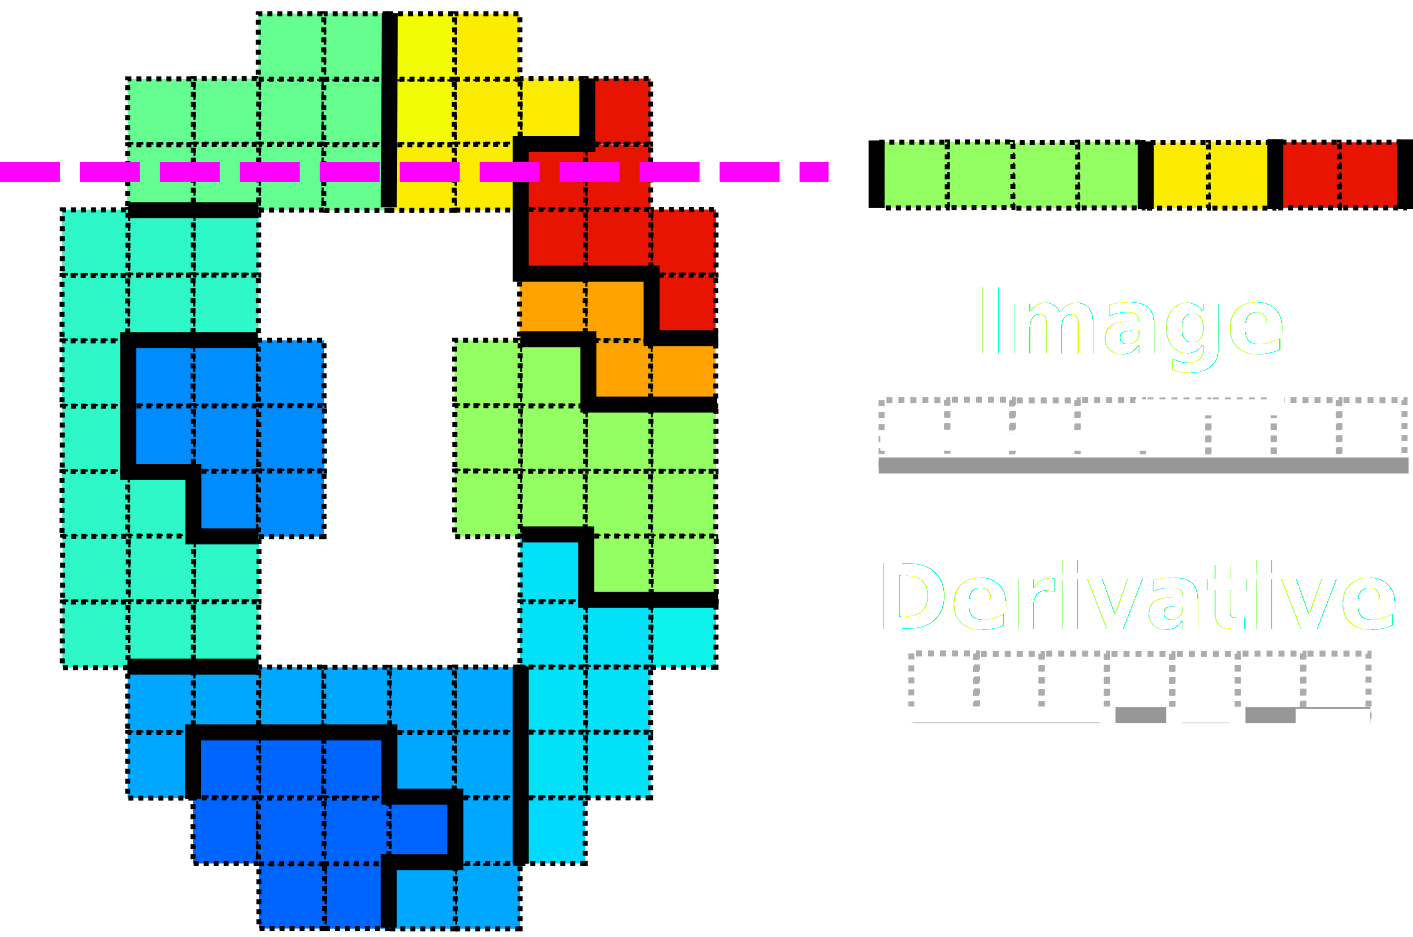
\includegraphics[width=1\linewidth]{figures/tv_cartoon_horizontal.png}
  \caption{A cartoon showing a sparse and blobby (step-wise constant / cartoon-like) brain map,
  as would be sought for by Total-Variation regularization \eqref{eq:ss}...}
  \label{fig:roi}
\end{marginfigure}
\begin{shaded}
\paragraph{Bayesian interpretation.} The penalties $\mathcal P(\w)$ in \eqref{eq:opt_pb} admit a Bayesian interpretation as a prior on the distribution of the coefficients $\w$
\begin{equation}
  \label{eq:bayesian}
  p_{\alpha,\rho}(\w) \propto \exp(-\mathcal P(\w)).
\end{equation}
For example, the GraphNet~\citep{grosenick2013,hebiri2011}, the penalties $\mathcal P(\w)$ penalty corresponds to
\begin{equation}
p_{\alpha,\rho}(\w) \propto    \prod_{j=1}^p\exp(-\alpha\rho |w_j|)\prod_{j=1}^p\exp\left(-\alpha(1-\rho)\sum_{l \sim \text{neigh}(j)}w_j\Delta_{j,l}w_l\right).
\end{equation}
\end{shaded}

The result of such regularized models, dubbed \emph{SpaceNet}
~\citep{spacenetohbm}, are brain maps which are both
sparse (i.e regression coefficients $\w$ are zero everywhere, except at
predictive voxels) and structured (blobby). See Fig. \ref{fig:roi}. The superiority of such
methods over methods without structured priors like the Lasso, ANOVA,
Ridge, SVM, etc. for yielding more intepretable maps and improved
prediction scores is now well established. See for example
  \citep{baldassarre2012,gramfort2013}. These priors are fast becoming
popular for brain decoding and segmentation. Indeed, they leverage a
feature-selection function
(since they limit the number of active voxels),
and also a structuring function
(since they penalize local
differences in the values of the brain map). For example, see Fig.
\ref{fig:spacenet_maps}.
Also, such priors produce state-of-the-art methods for automatic
extraction of functional brain atlases   \citep{abraham2013}.

\begin{shaded}
  \paragraph{Submodular interpretation of TV.} We note that anisotropic TV penalty \eqref{eq:penalty} on
  an arbitrary (undirected) graph $G = (V,E)$ is the \textit{Lovasz extension} of the \textit{cut-function}
  $F : 2^V \rightarrow \mathbb N$, $S \mapsto "\text{number of edges between } S \text{ and }V\setminus S"$,
defined by $F^L(x) := \mathbb E_{\lambda \sim \mathcal U([0,1])}[F(\{v \in V|x_v \ge \lambda\})]$, for all $x \in [0,1]^{\#V}$.
\end{shaded}

\begin{figure}[!htbp]
  \includegraphics[width=1\linewidth]{figures/haxby_barchart.png}
  \caption{Bar chart showing percentage classification on leftout, for one-vrs-one classification on the visual recognition dataset~\citep{haxby2001}.
  }
  \label{fig:spacenet_bars}
\end{figure}

\section{Methods}
The SpaceNet model leads to difficult non-smooth mathematical optimization problems making their implementation and practical usability challenging. \citep{dohmatob2014benchmarking} benchmarked a rich variety of cutting-edge solvers for such problems, and gave crucial recommendations on how to effectively implement these algorithms in practice. In these benchmarks, the FISTA algorithm emerged as the go-to algorithm for the TV-L1 problem~\citep{dohmatob2015speeding}. These hints have been carefully used in implementing SpaceNet. Also as a preprocessing step, we use univariate feature-screening (ANOVA) to eliminate voxels which are irrelevant to the learning problem, thus reducing the size of the problem. As a result the implementation of SpaceNet is fast, robust, and automatically sets its parameters (internal cross-validation). All these technical details will be properly presented in the next few chapters.

\section{Comparing SpaceNet with against basic models}
\paragraph{Classification.}
We compared SpaceNet (TV-L1 and Smooth-Lasso priors) with an SVM (Support Vector Machine) on the visual-recognition dataset~\citep{haxby2001}. This dataset consists of 6 subjects with 12 runs per subject. In each run, the subjects passively viewed images of eight object categories, grouped in 24-second blocks separated by intermittent rest periods. This experiment is a classification task: predicting the object category. The design matrix is made of time-series from the full-brain mask of $p=23,707$ voxels over 216 TRs (Repetition Times), of a single subject (subj1). 126 TRs were used for training all the models, whilst testing was done on 90 left-out TRs. The results are depicted in Figures 1 (bar chat) and 2 (brain maps).

\begin{figure}[!htb] 
  \includegraphics[width=.32\linewidth]{figures/svm.png}
  \includegraphics[width=.32\linewidth]{figures/graphnet.png}
  \includegraphics[width=.32\linewidth]{figures/tvl1.png}  
  \caption{The figure shows results of comparing the SpaceNet  models TV-$\ell_1$ and
    Graph-Net against an SVM (Support Vector Machine) classifier on
    the visual-recognition dataset   \citep{haxby2001}
    As can be seen from the figure, SpaceNet priors (TV-$\ell_1$, GraphNet, etc.)
    yield stable and more intepretable maps by enforcing smoothness on the coefficients while segmenting predictive regions (blobs) from noisy background.}
  \label{fig:spacenet_maps}
\end{figure}

\paragraph{Regression.}
In ~\citep{gramfort2013}, the authors compared several models on a dataset in which subjects were presented with mixed (gain/loss) gambles, and decided whether they would accept each gamble~\citep{jimura2012}. No outcomes of these gambles were presented during scanning, but after the scan three gambles were selected at random and played for real money. The prediction task here is to predict the magnitude of the gain and thus a regression on a continuous variable. The data is pooled across subjects, resulting in 768 samples, each an image of $p=33,177$ voxels. The results are shown in Fig. \ref{fig:tvl1_regression}.

\begin{figure}[!htb] 
  \includegraphics[width=1\linewidth]{figures/gramfort_tvl1.png}
  \caption{Results on fMRI data from [4] (from left to right F-test, ElasticNet and TV-L1). The TV-L1 regularized model segments neuroscientificly
    meaningful predictive regions in agreement with univariate statistics while the ElasticNet yields sparse although very scattered non-zero weights. Source: adapted from ~\citep{gramfort2013}.}
  \label{fig:tvl1_regression}
\end{figure}

\section{Conclusion}
We have presented SpaceNet, a family of priors for brain decoding which enforce both sparsity and structure, leading to better prediction scores and intepretable brain maps. We believe that such priors will become commonplace in future.
In the next chapter we open the ``black box'' and develop from ground-up, the details of such models, including their practical implementation on a computer.

% \clearpage
\bibliographystyle{plainnat}
\bibliography{bib_all}
 % SpaceNet model

\chapter{Efficient optimization of sparsity and smoothness regularized models}\label{chap:efficient_opt}
\markright{{~{\rm \ref{chap:efficient_opt}}. Algorithms for structured priors}\hfill}{}
\newthought{Though the SpaceNet model} presented above leads to superior estimators compared to classical estimators (Ridge regression, SVM, etc.) without spatial penalization, it is considerably harder to optimize than these classical models. Indeed, the corresponding optimization problems is non-separable in the model coefficients, and except for the case of GraphNet~\citep{hebiri2011,grosenick2013} and social-sparsity~\citep{kowalski2013social,varoquaux2016social},
the penalty term $\mathcal P(\w)$ is neither smooth nor proximable.
\footnote{ A function $f$ is said to be \textit{proximable} is the operator $\text{prox}_{\gamma f}$ is easy to compute. This is the case for $\ell_p$-norms  (with $ p \ge 1$, to ensure convexity) and indicator functions of simple closed convex sets like balls, simplexes, half-spaces, etc.}
For the penalty to fully exercise its
structuring effect on the maps, this optimization problem must be
solved to a good tolerance resulting in a computational challenge. Lack of good solver and explicit control of
tolerance can lead to brain maps and conclusions that reflect
properties of the solver more than of model coefficients, as illustrated in Fig. \ref{Fig:benchmarks_prni}.

  %% \begin{itemize}
  %% \item{proximal methods}
  %%   \begin{itemize}
  %%     \item single-step\\
  %%       {-} ISTA (Iterative Soft-Thresholding Algorithm)   \citep{daubechies2004}
  %%     \item multi-step / accelerated\\
  %%       {-} FISTA (Fast ISTA)   \citep{beck09fista}
  %%   \end{itemize}
  %% \item {primal-dual \& splitting methods}
  %%   \begin{itemize}
  %%   \item ADMM (Alternating Directions Method of Multipliers)   \citep{boyd2011distributed}
  %%     % (\textit{Alternating Directions Method of Multipliers})
  %%   \item Chambolle-Pock's Primal-Dual   \citep{chambolle2010}
  %%   \end{itemize}
  %% \item {quasi-Newton methods}
  %%   \begin{itemize}
  %%   \item HANSO ({Hybrid Algorithm for Non-smooth Optimization})   \citep{lewis2008}
  %%   \item L-BFGS   \citep{ciyou1994} on smooth surrogates of the penalty
  %%   \end{itemize}
  %% \end{itemize}
  

%% \begin{figure*}
%%   \begin{subfigure}[t]{1\linewidth}
%%     \hspace*{-.01\linewidth}%
%%     \includegraphics[width=.6\linewidth]{haxby_lr_energy.pdf}
%%     \hspace*{-.09\linewidth}%
%%     \includegraphics[width=.6\linewidth]{haxby_lr.pdf}%
%%     % \vspace{-2ex}
%%     \caption{\textbf{Classification} with logistic regression model
%%       \eqref{eq:opt_pb}. on the visual recognition face-house
%%     discrimination task. \textbf{Left}: excess energy $E(\mathbf{w}_t) -
%%     E(\mathbf{w})_{t \rightarrow \infty}$ as a function 
%%     of time.
%%     \textbf{Right}: convergence time of the various solvers for different
%%     choice of regularization parameters.
%%     Broken lines correspond to a tolerance of $10^{0}$,
%%     whilst full-lines correspond to $10^{-2}$.  The thick vertical line
%%     indicates the best model selected by cross-validation.}
%%     \label{Fig:HaxbyLR}
%%   \end{subfigure}
%%   \begin{subfigure}[t]{1\linewidth}
%%     \includegraphics[width=.6\linewidth]{haxby_mse.pdf}%
%%     \hspace{-.09\linewidth}%
%%     % generate with: ipython ../wip/tv_l1_solver/plot_parallel_plots.py poldrack_mse_12th.json 2e1 --pdb
%%     \includegraphics[width=.6\linewidth]{poldrack_mse.pdf}
%%     % \vspace{-2ex}
%%     \caption{\textbf{Regression.} results. \textbf{Left}:
%%       on the visual recognition  face-house discrimination task; \textbf{Right}: on the
%%       Mixed gambles dataset. Broken lines correspond to a tolerance of $10^{0}$,
%%       whilst full-lines correspond to $10^{-2}$. The thick vertical line
%%       indicates the best model selected by cross-validation.}
%%     \label{Fig:MSEtimes}
%%   \end{subfigure}
%% \caption{Benchmarks for different solvers for the TV-$\ell_1$ model
%%   \eqref{eq:opt_pb} on the visual recognition face-house
%%   discrimination task. See   \citep{dohmatob2014benchmarking} for more details.}
%% \end{figure*}

\section{Solving TV-L1 regularized problems}
\begin{figure}[!htb]
    \includegraphics[width=.331\linewidth]{face_vs_house_tol_0_1.pdf}%
\llap{\color{white}\raisebox{.17\linewidth}{\rlap{\sffamily Stopping:
      $\Delta E < 10^{-1}$}}\hspace*{.315\linewidth}}\hfill%
\includegraphics[width=.331\linewidth]{face_vs_house_tol_0_001.pdf}%
\llap{\color{white}\raisebox{.17\linewidth}{\rlap{\sffamily Stopping:
      $\Delta E < 10^{-3}$}}\hspace*{.315\linewidth}}\hfill%
\includegraphics[width=.331\linewidth]{face_vs_house_tol_1e-05.pdf}%
\llap{\color{white}\raisebox{.17\linewidth}{\rlap{\sffamily Stopping:
      $\Delta E < 10^{-5}$}}\hspace*{.315\linewidth}}%

\caption{TV-$\ell_1$ maps for the face-house discrimination task on
  the visual recognition dataset.
  Note that
  the stopping criterion is defined as a threshold on the energy
  decrease per one iteration of the algorithm, and thus differs from
  the tolerance displayed in figure \ref{Fig:benchmarks_prni}.  This figure shows
  the importance of convergence for problem \eqref{eq:opt_pb}, and motivates
  the need for fast solvers for SpaceNet priors, especially the non-smooth ones like TV-$\ell_1$ and Sparse Variation. See the full story in
  \citep{dohmatob2014benchmarking}}
  \label{Fig:benchmarks_prni}
\end{figure}
The optimization problem \eqref{eq:opt_pb} is very challenging:
it is non-smooth (except in the case of Laplacian regularization), non-separable and heavily ill-conditioned. For the penalty to fully exercise its
structuring effect on the maps, this optimization problem must be
solved to a good tolerance resulting in a computational challenge.
In \citep{dohmatob2014benchmarking}, we did an extensive study of all solvers applicable to the problem in TV-$\ell_1$ special case (which happens to be the most difficult scenario).
Our results outlined the best strategy: a double FISTA loop, where the
inner loop computes the proximal operator of the penalty term, with approximate precision on the duality-gap. This was further refined and implemented in   \citep{varoquaux2015faasta}.

% In  \citep{dohmatob2014benchmarking}, we explored a wide variety of solvers and exhibited their
% convergence properties on fMRI data. Below we present a brief overview of the paper.

\subsection{The algorithms}
\paragraph{ISTA/FISTA.}
ISTA~ \citep{daubechies2004}, and its accelerated variant
FISTA~ \citep{beck2009a}, are proximal gradient approaches: the go-to
methods for non-smooth optimization. In their seminal introduction of TV
for fMRI,  \citep{michel2011} relied on ISTA.
The challenge of these methods for TV is that the proximal operator
%% \footnote{The proximal operator (or prox for short) can be seen as a generalization of projection unto convex set.}
  of TV
cannot be computed exactly; we approximate it in an inner FISTA loop
 \citep{beck2009b,michel2011}.
% ,  \citep{gramfort-etal:2013a}.
%%  and must itself be solved by a
%% FISTA\footnote{Note that solving TV and TV$-\ell_1$ are formally very
%% close  \citep{gramfort-etal:2013a}.
% }
%  \citep{beck2009b,michel2011}. 
Here, for all FISTA implementations we use
the faster monotonous FISTA variant  \citep{beck2009b}. We control the
optimality of the TV proximal via its dual gap  \citep{michel2011} and
use a line-search strategy in the monotonous FISTA to decrease the
tolerance as the algorithm progresses, ensuring convergence of the
TV-$\ell_1$ regression with good accuracy.

\paragraph{ISTA/FISTA with backtracking.}
A key ingredient in FISTA's convergence is the Lipschitz
constant $L_{\nabla \ell}$, of the derivative of smooth part of the objective function
. The tighter the upper bound used for this constant,
the faster the resulting FISTA algorithm. In FISTA, the main use of 
$L_{\nabla \ell}$ is the fact that: for any
stepsize $0 < t \le 1/L_{\nabla \ell}$ and for any point $\mathbf{z}$,
\begin{shaded}
\begin{equation}%
  \begin{gathered}
    \ell(\mathbf{p}_{t}(\mathbf{z})) \le
    \ell(\mathbf{z}) + \mathbf{r}_{t}^T\nabla
    \ell(\mathbf{z}) + \frac{1}{2t} \|\mathbf{r}_{t}\|_{2}^2,
    \text{  where} \quad\\
    \mathbf{p}_{t}(\mathbf{z}) := \textrm{prox}_{\alpha t J}(\mathbf{z} - t
    \nabla \ell(\mathbf{z})) \,\text{  and  }\,
    \mathbf{r}_{t} :=
    \mathbf{p}_{t}(\mathbf{z}) - \mathbf{z} \quad
  \end{gathered}
  \label{eq:fista_ineq}
\end{equation}
\end{shaded}
In least-squares regression, $L_{\nabla \ell}$ is precisely the largest
singular value of the design matrix $\mathbf{X}$.
For logistic
regression however, the tightest known upper bound for
$L_{\nabla \ell}$ is $\|\mathbf{X}\|\|\mathbf{X}^T\|$,
% (for example see Appendix A of  \citep{yuan2012}),
which performs very poorly locally (i.e, stepsizes $\sim 1 / L_{\nabla \ell}$ are
sub-optimal locally). A way to circumvent this difficulty is
\emph{backtracking line search}  \citep{beck2009a}, where one tunes the
stepsize $t$ to satisfy inequality \eqref{eq:fista_ineq} locally at
point $\mathbf{z}$. 


\paragraph{ADMM: Alternating Direction Method of Multipliers.}
ADMM is a Bregman Operator Splitting primal-dual method for
solving convex-optimization problems by splitting the
objective function in two convex terms which are functions of linearly-related auxiliary variables
 \citep{boyd2010}.  ADMM is particularly appealing for problems such as TV
regression: using the variable split $\mathbf{z}
\leftarrow \nabla \mathbf{w}$, the regularization is a simple $\ell_{1}/\ell_2$
norm on $\mathbf{z}$ for which the proximal is exact and computationally
cheap. However, in our settings, limitations of ADMM are:
\begin{itemize}
\item The $\mathbf{w}$-update involves the inversion of a large $p$-by-$p$
  ill-conditioned linear operator (precisely a weighted sum of
  $\mathbf{X}^T\mathbf{X}$, the laplacian $\Delta$, and the identity
  operator).
\item The $\rho$ parameter for penalizing the split
  residual $\mathbf{z} - \nabla \mathbf{w}$ is hard to set (this is still an
  open problem), and though under mild conditions ADMM
  converges for any value of $\rho$, the convergence rate depends
  on $\rho$.
\end{itemize}

\paragraph{Primal-Dual algorithm of Chambolle and Pock  \citep{chambolle2010}.}
this scheme is another method based on operator splitting.
Used for fMRI TV regression by  \citep{gramfort-etal:2013a},
it does not require setting a hyperparameter.  % XXX : this is wrong you have the tau / sigma
However it is a first-order single-step method and is thus more impacted by the
conditioning of the problem. Note that here we explore this primal-dual
method only in the squared loss setting, in which the algorithm can be accelerated by
precomputing the SVD of $\mathbf{X}$  \citep{gramfort-etal:2013a}
.

\paragraph{HANSO  \citep{lewis2008}.}
a modified LBFGS scheme based on gradient 
sampling methods  \citep{burke2005} and inexact
line-search. For non-smooth problems as in our case, the algorithm relies on
random initialization, to avoid singularities with high probability. 
Here, we used the original authors' implementation.

\paragraph{Uniform approximation by smooth convex surrogates.}
The $\ell_{1}$ norm (resp. TV semi-norm) is differentiable everywhere with
gradient $\left(w_j/|w_j|\right)_{j \in [\![p]\!]}$ (resp. $-\dive (((\nabla \mathbf{w})_j/\|(\nabla \mathbf{w})_j\|_2)_{j \in [\![p]\!]}))$), except when some voxels are inactive with
$w_j = 0$ (resp. $(\nabla \w)_j = 0$), corresponding to black spots (resp. edges).  A convenient
approach (see for example  \citep{NESTA, nesterov2005a, nesterov2005b,
  beck2012}) for dealing with such singularities is to uniformly
approximate the offending function with smooth surrogates that
preserve its convexity. Given  % I removed "and other important properties"
a smoothing parameter $\mu > 0$, we define \emph{smoothed} versions
of $\ell_1$ and TV:
%
\begin{eqnarray}
    \|\mathbf{w}\|_{1,\mu} := \sum_j
    \sqrt{\mathbf{w}_j^2 + \mu^2},\;
    \|\mathbf{w}\|_{\text{TV}, \mu} :=
    \sum_{j} \sqrt{\|\nabla \mathbf{w}_j\|_{2}^2 + \mu^2}
\end{eqnarray}
These surrogate upper-bounds are convex and everywhere-differentiable
with gradients that are Lipschitz-continuous with constants $1/\mu$ and
$\|\nabla\|^2(1/\mu) = 12 / \mu$ respectively.
They lead to smoothed versions of problem \eqref{eq:opt_pb}:
\begin{align}
  \mathbf{\hat{w}}_{\mu} := \argmin_{\mathbf{w}}\;
  \{E_{\mu}(\mathbf{w}) := \ell(\mathbf{w}) + \alpha
    \mathcal P_{\text{TV-L1},\mu}(\mathbf{w})\},
  \label{eq:sopt_pb}
\end{align}
where    $\mathcal P_{\text{TV-L1},\mu}(\mathbf{w}) :=\rho \|\mathbf{w}\|_{1,\mu} +
(1 - \rho)\|\mathbf{w}\|_{\text{TV}, \mu}$.

To solve \eqref{eq:opt_pb}, we consider problems of the form
\eqref{eq:sopt_pb} with $\mu \rightarrow 0^+$: we start with a coarse
$\mu$ ($= 10^{-2}$, \emph{e.g}) and cheaply solve the $\mu$-smoothed problem
\eqref{eq:sopt_pb} to a precision $\sim \mu$ using a fast
iterative oracle like the LBFGS \citep{ciyou1994}; we
obtain a better estimate for the solution; then we decrease $\mu$ by a fixed factor,
and restart the solver on problem \eqref{eq:sopt_pb} with this solution; and so on, in a 
\emph{continuation} process~\citep{NESTA} detailed in Alg.
\ref{Tab:pseudocode_lbfgs}.
This algorithm is not faster than
$\mathcal{O}(1/\epsilon)$: indeed a good optimization algorithm
for the sub-problem \eqref{eq:sopt_pb} is $\mathcal{O}(\sqrt{L_{\mu}/\epsilon})$
\citep{nesterov1983}, and $L_{\mu} \sim 1 / \mu \sim 1 / \epsilon$. We
believe that this bound is tight but a detailed analysis is
beyond the scope of this paper.
\begin{algorithm}
  \caption{LBFGS algorithm with continuation}
  \label{Tab:pseudocode_lbfgs}  
  \begin{algorithmic}[1]  
    \Require $\epsilon > 0$ the desired precision, $\beta$ ($0 < \beta <
    1$) the rate of decay of the smoothing parameter $\mu$, and $\gamma > 0$ be a constant.
    Finally,
    let LBFGS: $(E_\mu, \mathbf{w}^{(0)}, \epsilon) \mapsto \mathbf{w}$ be
    an oracle which when warm-started with an initial guess
    $\mathbf{w}^{(0)}$, returns an $\epsilon$-optimal
    solution (i.e $E_\mu(\mathbf{w}) - E_\mu^{*} < \epsilon$) for problem \eqref{eq:sopt_pb}.\\
    \textbf{Initialize} $ 0 < \mu^{(0)}$ ($= 10^{-2}$, \emph{e.g}),
    $\mathbf{w}^{(0)}\in \mathbb{R}^p$, and $k = 0$.
    \While{$\gamma\mu^{(k)} \ge \epsilon$}
    \State $\mathbf{w}^{(k + 1)} \leftarrow \mbox{LBFGS}(E_{\mu^{(k)}}, \mathbf{w}^{(k)}, \gamma\mu^{(k)})$
    \State $\mu^{(k + 1)} \leftarrow \beta \mu^{(k)}$
    \State $k \leftarrow k + 1$
    \EndWhile
  \end{algorithmic}
\end{algorithm}

\subsection{Experiments on fMRI datasets}
\label{sec:experiments}
We now detail experiments done on publicly available
data. All experiments were run full-brain without spatial smoothing.

\paragraph{Visual recognition.}
\label{subsec:haxby}
Our first benchmark dataset is a popular block-design fMRI dataset from a study on face and
object representation in human ventral temporal cortex  \citep{haxby2001}.
It consists of
6 subjects with 12 runs per subject. In each run, the subjects
passively viewed images of eight object categories, grouped
in 24-second blocks separated by intermittent rest periods. This
experiment is a classification task: predicting the object category. We use a
two-class prediction target: $\mathbf{y}$ encodes faces versus houses.
The design matrix $\mathbf{X}$ is made of
time-series from the full-brain mask of $p = 23\,707$ voxels over $n =
216$ TRs, of a single subject (subj1).

\paragraph{Mixed Gambles.}
Our second benchmark dataset is a study in which
subjects were presented with mixed (gain/loss) gambles, and decided
whether they would accept each gamble \citep{mixedgambles2007}.  No outcomes of these gambles
were presented during scanning, but after the scan three gambles were
elected at random and played for real money. The prediction task here is
to predict the magnitude of the gain and thus a regression on a
continuous variable \citep{jimura2012}. The data is pooled across
subjects, resulting in 768 samples, each an image of 33\,177 voxels.

% We validate our algorithms on both simulated and real data.
\smallskip

We study the convergence of the algorithms for parameters close to the
optimal parameters set by 10-fold cross-validation to maximize prediction
accuracy.

\subsection{Results: convergence times}
 \begin{figure}[!htbp]
   \includegraphics[width=1\linewidth]{figures/solvers_1.png}
   \includegraphics[width=1\linewidth]{figures/solvers_2.png}
   \caption{\textbf{Benchmarking } solvers for TV-$\ell_1$ penalized models. \textbf{Top:} TV-$\ell_1$ penalized Logistic Regression on the visual recognition face-house discrimination task. \textbf{Top Left:} excess energy $E(\B{w}_t ) - E(\B{w}^*)$ as a function of time. \textbf{Top Right:} convergence time of the various solvers for different choice of regularization parameters. Broken lines correspond to a tolerance of
     $10^0$ , whilst full-lines correspond to $10^{-2}$ . The thick vertical line indicates the best model selected by cross-validation. \textbf{Bottom:} TV-$\ell_1$ penalized Least-Squares Regression. \textbf{Bottom Left:} on the visual recognition face-house discrimination task; \textbf{Bottom Right:} on the Mixed gambles dataset. The thick vertical line indicates the best model selected by cross-validation.}
   \label{fig:tvl1bench}
\end{figure}

\label{sec:results}
Here, we present benchmark results for our experiments. Figure
\ref{Fig:HaxbyLR} gives results for the logistic regression run on the
visual recognition dataset: convergence plots of energy as a function of
time show that all methods are asymptotically decreasing. The left part of
Fig. \ref{fig:tvl1bench}
shows the time required to give a convergence
threshold, defined as a given excess energy compared to the lowest energy
achieved by all methods, for different choices of regularization
parameters. Similarly, the right part of Fig. \ref{fig:tvl1bench} shows convergence times
for squared loss on both datasets. For these figures,
each solver was run for a maximum of 1 hour per problem. Solvers that do
not appear on a plot did not converge for the corresponding
tolerance and time budget.

For logistic loss, the most serious contender is
algorithm \ref{Tab:pseudocode_lbfgs}, LBFGS applied on a smooth
surrogate, followed by ADMM, however ADMM performance
varies markedly depending on the choice of $\rho$. For the squared loss
FISTA and algorithm \ref{Tab:pseudocode_lbfgs} are the best performers,
with FISTA achieving a clear lead for the larger mixed-gambles dataset.
Note that in the case of strong regularization the problem is better
conditioned, and first-order methods such as the
primal-dual approach can perform well.

\section{More speed via univariate feature-screening and early-stopping}
In our PRNI 2015 conference paper   \citep{dohmatob2015speeding}, we presented some heuristics for speeding up the overall optimization process: (a) Early-stopping, whereby one  halts
the optimization process when the test score (performance on left-out
data) for the internal cross-validation for model-selection stops
improving, and (b) univariate feature-screening, whereby irrelevant
(non-predictive) voxels are detected and eliminated before the
optimization problem is entered, thus reducing the size of the
problem.

Empirical results with GraphNet on real MRI (Magnetic
Resonance Imaging)
datasets indicated that these heuristics are a win-win strategy, as
they add speed without sacrificing the quality of the predictions
/ classifications.

 \begin{figure}[!htb]
   \includegraphics[width=1\linewidth]{figures/screening.png}
\caption{Univariate feature-screening for the
  GraphNet~\citep{hebiri2011,grosenick2013}
  problem \eqref{eq:opt_pb} on
  different datasets.
  % $(\X,\y)$.
  This figure shows spatial maps of
  $\B{X}^T_j\y$, thresholded so that only voxels $j$ with (from left to
  rightmost column)  $|\B{X}^T_j\y| \ge p_{10\%}(|\B{X}^T\y|)$, $|\B{X}^T_j\y| \ge
  p_{20\%}(|\B{X}^T\y|)$, $|\B{X}^T_j\y| \ge p_{50\%}(|\B{X}^T\y|)$, and $|\B{X}^T_j\y|
  \ge p_{100\%}(|\B{X}^T\y|)$ (full-brain) respectively, survive. The
  green contours enclose the elite voxels which are selected by the
  screening procedure at the respective threshold
  levels. \textit{(a)}: Mixed Gambles dataset
   \citep{jimura2012}.%  Remarkably, the geometry of the regions obtained
  % here for the 10th and 20th screening-percentiles match pretty well
  % the results obtained in  \citep{gramfort2013} with their TV-L1
  % penalty. \textit{(b)}: Face vs House contrast of the visual recognition
  % dataset  \citep{haxby2001}. 
  Weights maps obtained for the GraphNet
  model \eqref{eq:opt_pb} with these different
  screening-percentiles are shown in Figure
  \ref{fig:haxby}. \textit{(c)}: OASIS dataset  \citep{marcus2007open}
  with VBM. See Figure \ref{fig:oasis} for weights maps and
  age predictions obtained using these different
  screening-percentiles. % on the GraphNet model \eqref{eq:opt_pb}.
}

\label{fig:screening}
\end{figure}

\subsection{Methods}
%% We will now detail the heuristic techiques for speeding up
%% numerical optimization of GraphNet  \citep{hebiri2011,grosenick2013}
%% model for brain data.


% \paragraph{A note on implementation of the solver.}
One notes that in the case of GraphNet, the penalty term % $J(\w)$
of problem
\eqref{eq:opt_pb}, the $\|\nabla
\w\|^2_2$ sub-term is smooth (i.e differentiable) with
\textit{Lipschitz} gradient, whilst the $\ell_{1}$ term though
nonsmooth, is \textit{proximable}\footnote{That is, there is a
  closed-form analytic expression for its proximal operator.} by means
of the \textit{soft-thesholding} operator  \citep{daubechies2004}.  Thus
problem \eqref{eq:opt_pb} is amenable to the FISTA (Fast Iterative
Shrinkage-Thresholding Algorithm)  \citep{beck09fista}, with a provable
$\mathcal{O}(1/\sqrt{\epsilon})$ convergence rate. Our implementation
of FISTA uses technical recommendations
(line-searching, parametrization, etc.) which were provided in
 \citep{dohmatob2014benchmarking}, in the context of TV-L1
 \citep{baldassarre2012,gramfort2013}. The model parameters $\alpha$ and
$\rho$ in \eqref{eq:opt_pb} are set by \textit{internal}
cross-validation.

%% \paragraph*{(b) Warm-start}
%% The $(\alpha, \rho)$ parameter grid is walked $\rho$-first. For each $\rho$ value encountered, the alphas are walked from largest to smallest value. The largest value is contructed to be the largest value of $\alpha$ for which the optimal solution to problem \eqref{eq:opt_pb} is necessarily zero.

%% We now provide details on the speedup heuristics for speeding up
%% the overall implementation, including model-selection part of it.


\paragraph{Univariate feature-screening.}
%% \textbf{XXX: In a paragraph briefly give a comprehensive overview of
%%   screening algorithms and heuristics from El Ghaoui, upto the more
%%   recent Liu et al!!!}
In machine-learning, feature-screening aims at detecting and
eliminating irrelevant (non-predictive)
features thus reducing the size of the underlying
optimization problem (here problem \eqref{eq:opt_pb}). The general idea
is to compute for each value of the regularization parameter, a
\textit{relevance measure} for each feature, which is then compared with a
threshold (produced by the screening procedure itself). Features which fall short
of this threshold are detected as irrelevant and eliminated. For the
Lasso and similar models (including Group Lasso),
\textit{exact}
screening techniques (i.e, techniques
  which don't mistakenly discard active predictive features) include those developed in
 \citep{elghaoui2010,lee2014exact,liu2014safe,wang2015lasso}. Inexact
screening techniques (e.g  \citep{tibshirani2010strong}) have also been
proposed in the literature.
Our proposed heuristic screening technique is inspired by the
\textit{Marginal screening} technique developed in Algorithm 1 of
 \citep{lee2014exact}, and operates as
follows. The data $(\X,\y)$ are standardized so that $\y$ has unit
variance and zero mean, likewise each row of the design matrix $\X$. To
ensure obtention of a smooth mask, a Gaussian-smoothed version
of $\X$ is used in the screening procedure (but not in the actual model
fit).
For each voxel $j$ (voxels are the features here) the
absolute dot-product $|\B{X}^T_j\y|$ of $\y$ with the $j$th column of
$\X$ is computed.
% This is used as the relevance measure.
For a given screening-percentile
$sp \in [0, 100]$ , the $sp$th percentile value of the
vector $|\B{X}^T\y| := (|\B{X}^T_1\y|, ..., |\B{X}^T_p\y|)$, denoted $p_{sp}(|\B{X}^T\y|)$,
is computed. The case $sp=100$ corresponds to full-brain analysis. 25
means we keep the quarter of the brain made of voxels with the highest
$|\B{X}^T_j\y|$ values, and so on.
% ; this is the threshold.
A brain-mask is then formed containing only those voxels $j$
for which $|\B{X}^T_j\y| \ge p_{sp}(|\B{X}^T\y|)$. Next, this brain-mask is
morphologically eroded
% (to remove isolated small patches)
and then
dilated, to obtain a more structured mask.  Figure
\ref{fig:screening} shows results of applying this screening heuristic
to various datasets, prior to model fitting.

\subsection{Experiments}
We experimented our early-stopping and (separately)
feature-screening heuristics on different MRI datasets.
All experiments were run using a single core of
  a laptop.

\paragraph{Regression.} The OASIS dataset
     \citep{marcus2007open} consists of a
    cross-sectional collection of 416 subjects aged 18 to 96. For each
    subject, 3 or 4 individual T1-weighted MRI scans obtained in
    single scan sessions are included.   A natural regression problem
    for this dataset is to predict the age of a subject from their
    anatomical data. To this end, we segmented the gray-matter from
    the anatomy of each subject (obtained from the T1 images), and
    used the gray-matter maps
    as features for predicting age. We split the 416 subjects into two
    equally-sized and age-balanced groups: a train set and a validation
    set. The GraphNet model  \citep{hebiri2011,grosenick2013} was fitted
    on the train set, with parameters
    ($\alpha$ and $\rho$ in \eqref{eq:opt_pb}) set internally via 8-fold
    cross-validation. The results for this experiment are shown in
    Figure \ref{fig:oasis}.

\paragraph{Classification.} The visual
    recognition dataset  \citep{haxby2001} is a popular block-design
    fMRI dataset from a
    study on face and object representation in human ventral temporal
    cortex.
It consists of 6 subjects with 12 runs per subject. In each run, the
subjects
passively viewed images of eight object categories, grouped
in 24-second blocks separated by intermittent rest periods. This
experiment is a classification task: predicting the object category
$\y$. We use a \textit{One-versus-Rest (OvR)} strategy. The design
matrix $\B{X}$ is made of
time-series from the full-brain mask of $p = 23\,707$ voxels over $n =
216$ TRs, of a single subject (subj1). We divided the 12 runs into 6
runs for training and 6 other runs for
validation. \textit{Leave-one-label-out} cross-validation was used for
selecting the model parameters $(\alpha, \rho)$. The results are
depicted in Figure \ref{fig:haxby}.

\subsection{Results.}
We now summarize and comment the results of the experiments (refer to
section \ref{sec:experiments}).
Figure \ref{fig:oasis} shows the effects of early-stopping heuristic
and feature-screening heuristic on age prediction scores on the OASIS
dataset  \citep{marcus2007open} (416 subjects). We see that in the
internal cross-validation, stopping  the optimization procedure for
fixed $(\alpha, \rho)$ pair of regularization parameters, when test
score increases by $-10^{-2}$ or more is a good heuristic, and does just
as good as running the optimization until numerical convergence. 
 \begin{figure}[!htb]
   \includegraphics[width=1\linewidth]{figures/screening_weights.png}
  \caption{Predicting age from gray-matter concentration maps from the
    OASIS dataset  \citep{marcus2007open}. \textbf{Top}:
    Weights maps (solutions to problem \eqref{eq:opt_pb}).
% \textbf{N.B}: The long spiky undershoots in the prediction curves
% are indicative of outliers: subjects for which spatial preprocessing
% (tissue segmentation, normalization, etc.) failed.
\textbf{Bottom-left}: Mean Square Error (MSE) in age prediction, for
different subjects of the validation set, for  varying levels of the
early-stopping tolerance (``es tol'' for short), with the
screening-percentile (sp) held constant at 100
(full-brain). \textbf{Bottom-right}: MSE in age prediction, for
varying levels of the screening-percentile (sp).%  \textbf{Running
%   times}: Increasing \textit{est tol} (from $-10^{-4}$ to $10$): \textbf{100.2m, 171.4m, 188.8m, 289.6m}. For
% increasing $sp$ ($10$ to $100$): \textbf{44.2m, 81.3m, 186.5m, 341.3m}
}   
\label{fig:oasis}
\end{figure}
Also (and independently), one gets similar prediction scores using as
little as a fifth of the brain volume ($sp=20$),
compared to using the full-brain ($sp=100$).
Figure \ref{fig:haxby} reports similar results for classification on
the visual recognition dataset  \citep{haxby2001}. Overall, we see from
Figures \ref{fig:haxby} and \ref{fig:oasis} that we can achieve upto
$10$-fold speedup with the proposed heuristics, with very little loss
in accuracy. Also, we see that contiguous groups of bars are roughly flat at the top, with a
    sligh increase from lower to high screening-percentile values. The
    case ``chair vs scramped'' is an exception, where a slightly reverse tendency
    if observed. A possible explanation is that $20$th percentile
    feature-screening already selects the right voxels (quasi-exact
    support recovery), and so including more voxels in the model can only hurt its
    performance...    

 \begin{figure}[!htb]
   \includegraphics[width=1\linewidth]{figures/screening_weights_haxby.png}
  \caption{Predicting age from gray-matter concentration maps from the
    OASIS dataset  \citep{marcus2007open}. \textbf{Top}:
    Weights maps (solutions to problem \eqref{eq:opt_pb}).
% \textbf{N.B}: The long spiky undershoots in the prediction curves
% are indicative of outliers: subjects for which spatial preprocessing
% (tissue segmentation, normalization, etc.) failed.
\textbf{Bottom-left}: Mean Square Error (MSE) in age prediction, for
different subjects of the validation set, for  varying levels of the
early-stopping tolerance (``es tol'' for short), with the
screening-percentile (sp) held constant at 100
(full-brain). \textbf{Bottom-right}: MSE in age prediction, for
varying levels of the screening-percentile (sp). \textbf{Running
  times}: Increasing \textit{est tol} (from $-10^{-4}$ to $10$): \textbf{100.2m, 171.4m, 188.8m, 289.6m}. For
increasing $sp$ ($10$ to $100$): \textbf{44.2m, 81.3m, 186.5m, 341.3m}}   
  \caption{Visual recognition dataset
     \citep{haxby2001}. \textbf{\textit{(a)}}: Weights maps
    % (maps of
    % regression coefficients $\hat{w}$)
    for the Face vs House contrast,
    for different early-stopping and univariate feature-screening
    thresholds. One can see that the supports of these maps for
    different values of the thresholds are quite similar to cases
    involving  no heuristic at all (the case where est $= 10$ and the
    where case sp $=100\%$).
    \textbf{\textit{(b)}, top-left}: Prediction scores as a function of
    the early-stopping tolerance (est), for different task contrasts.
    \textbf{\textit{(b)}, top-right}: Prediction scores as a function of
    the screening-percentile (sp), for different task contrasts.
    \textbf{\textit{(b)}, bottom-row}: Running times in minutes for the
    different thresholds of the heuristics.
    % As was to be expected, full-brain
    % (sp=100\%) is the most expensive scenario.
  }
  \label{fig:haxby}
\end{figure}
    
 In   \citep{dohmatob2015speeding}, we empirically showed on various
datasets that such screening leads to linear speed-up in the computation
time, while sacrificing prediction / classification power as long as the
screening is not very savage. We also showed that early-stopping the
estimator does not harm the accuracy of the predictions, and can also lead
to considerable (though less systematic speedups).
The result of these numerous ramblings on optimizing the SpaceNet model \eqref{eq:opt_pb} have been implemented as part of the \textit{Nilearn} package   \citep{nilearn}.


% \newthought{We have seen} in Chapter~\ref{chap:stats_fmri} that%  encoding and decoding models take 
% as input  brain activation coefficients (also known as activation patterns or beta-maps). These are usually computed by means of the general linear model (GLM), which
% relies on a \mbox{data-independent} \emph{canonical} form of the hemodynamic response function
% (HRF).


% In this chapter we describe a novel method for the simultaneous estimation of HRF and activation coefficients based on low-rank modeling, forcing the estimated HRF to be equal across events or experimental conditions,
%  yet permitting it to differ across voxels. The estimation of this model leads to
% an optimization problem that we propose to solve with using a
% \mbox{quasi-Newton} method, exploiting fast gradient computations. 
% We compare 10 different HRF modeling methods in terms of encoding and decoding
% score on two different datasets. These results show that the \mbox{R1-GLM} model
% outperforms competing methods in both encoding and decoding
% settings, positioning it as an attractive method both from the points of view
% of accuracy and computational efficiency.

% \hspace{20pt}
% \begin{shaded}
% The contributions developed in this chapter have been published in:
% \begin{itemize}
% \item F. Pedregosa, M. Eickenberg, P. Ciuciu, and B. Thirion, \emph{``Data-driven HRF estimation for encoding and decoding models''} NeuroImage, Volume 104, 1 January 2015, Pages 209-220.

% \item F. Pedregosa, M. Eickenberg, B. Thirion, and A. Gramfort, \emph{“HRF estimation improves sensitivity of fMRI encoding and decoding models”} Proc. 3nd Int. Work. Pattern Recognit. NeuroImaging, 2013.
% \end{itemize}
% \end{shaded}

% \newpage
% \vspace*{\fill}
% \minitoc
% \vspace*{\fill}
% \newpage


% \section{Sparsity and smoothness priors for improved estimation in high dimensions}
% \newthought{Michel et al. 2011, Baldasarre et al. 2012, Gramfort et al. 2013, Abraham et al. 2013, Dohmatob et al. 2014(5), Varoquaux et al. 2016}, ...

% \begin{marginfigure}[4cm]
% \hspace{-20pt}\includegraphics[width=1.2\linewidth]{chapter_3/hrfs_age.pdf}
% \caption{
% 	The HRF can vary substantially between subjects, brain regions and age. In  \citept{colonnese2007development}, the authors studied the evolution of the HRF across age in rats. By comparing fMRI measurements with electrophysiological recordings, they observed two significant trends as age increased: growing amplitude and decreasing time to peak. In the figure, estimated HRF for three groups of rats (with age P13-15 < P20-30< Adult). Source:  \citepp{colonnese2007development}. A comparison of the HRF in human subjects was performed in~ \citepp{badillo2014multi}.
% }
% \end{marginfigure}


% fMRI acquisitions consist of successive brain scans, given in intervals ranging from 1 to 4 seconds. The extraction of time-independent \gls{activation coefficient} from the BOLD time course is commonly done with a model known as Linear General Model
% (GLM)~ \citepp{Friston1995}. While
% this approach has been successfully used in a wide range of studies, it does
% suffer from limitations~ \citepp{Poline2012}. For instance, the GLM commonly
% relies on a \mbox{data-independent} \emph{reference} form of the hemodynamic response function
% (HRF) to estimate the activation coefficient (also known as \emph{canonical HRF}). However it is
% known~ \citepp{Handwerker2004,Badillo2013} that the shape of this response function
% can vary substantially across subjects, age and brain regions. This suggests that an adaptive modeling of this
%  response function should improve the accuracy of subsequent analysis.

% % \emph{feature-extraction} model that extracts 

% % In this section we describe a method that allows to estimate time-independent \gls{activation coefficient} given the BOLD time course. {\blue Feature extraction}. This model is known as the \emph{general linear model}~ \citepp{Friston1995}. In this chapter we describe the main assumptions behind this model: a known form of the hemodynamic response function and the linear-time-invariant property between the BOLD signal and the neural response. 

% % We have seen in Chapter 2 that both encoding and decoding models take as input voxel-wise activation coefficients. These are commonly are computed by means of the General Linear Model
% % (GLM)~ \citepp{Friston1995}. While
% % this approach has been successfully used in a wide range of studies, it does
% % suffer from limitations~ \citepp{Poline2012}. For instance, the GLM commonly
% % relies on a \mbox{data-independent} \emph{reference} form of the hemodynamic response function
% % (HRF) to estimate the activation coefficient (also known as \emph{canonical HRF}). However it is
% % known~ \citepp{Handwerker2004,Badillo2013} that the shape of this response function
% % can vary substantially across subjects, age and brain regions. This suggests that an adaptive modeling of this
% %  response function should improve the accuracy of subsequent analysis.

% To overcome the aforementioned limitation, Finite Impulse Response (FIR) models have been
% proposed within the GLM framework~ \citepp{Dale1999,Glover1999}.
% These models do not assume any particular shape for the HRF and amount to
% estimating a large number of parameters in order to identify it. 
% While the FIR-based modeling makes it possible to estimate the
% activation coefficient and the HRF simultaneously, the increased flexibility
% has a cost. The estimator is less robust and prone to overfitting, i.e. to generalize poorly to unseen data. 
% In general, FIR
% models are most appropriate for studies focused on the characterization of the
% shape of the hemodynamic response, and not for studies that are primarily
% focused on detecting activation~ \citep[Chapter~5]{Poldrack}.

% Several strategies aiming at reducing the number of degrees of freedom of the
% FIR model - and thus at limiting the risk of overfitting - have been proposed.
% One possibility is to constrain the shape of the HRF to be a linear
% combination of a small number of basis functions. A common choice of basis is 
% formed by three elements consisting of a reference HRF as well as its time and dispersion
% derivatives~ \citepp{friston1998nonlinear}, although it is also possible to compute a
% basis set that spans a desired function
% space~ \citepp{Woolrich2004}. More generally, one can also define a parametric
% model of the HRF and estimate the parameters that best fit this
% function~ \citepp{Lindquist2007}. However, in this case the estimated HRF may no longer be a linear function of the input parameters. 

% Sensitivity to noise and overfitting can also be reduced through
% regularization. For example, temporal regularization has been used in the
% smooth FIR ~ \citepp{Goutte2000,Ciuciu2003,Casanova2008} to favor solutions with
% small second order time derivative. These approaches require the setting of
% one or several hyperparameters, at the voxel or potentially at the parcel
% level (if several voxels in a pre-defined parcel are assumed to share some aspects of the HRF time course). Even if efficient techniques such as generalized   
% \mbox{cross-validation}~ \citepp{golub1979generalized} can be used to choose the
% regularization parameters, these methods are inherently more costly than 
% \mbox{basis-constrained} methods. \mbox{Basis-constrained} methods also require
% setting the number of basis elements; however, this parameter is not
% continuous (as in the case of regularized methods), and in practice only few
% values are explored: for example the 3-element basis set formed by a reference HRF
% plus derivatives and the FIR model.  This paper focuses on basis-constrained
% regularization of the HRF to avoid dealing with hyperparameter selection with
% the goal of remaining computationally attractive.  A different approach to
% increase robustness of the estimates consists in linking the estimated HRFs
% across a predefined brain parcel, taking advantage of the spatially dependent nature of
% fMRI~ \citepp{Wang2013}. However, \mbox{hemodynamically-informed}
% parcellations~ \citepp{Chaari2012,Badillo2013a} rely on the computation of 
% a large number of estimations at the voxel or \mbox{sub-parcel} level.
% In this setting, the development of voxel-wise estimation procedures is complementary to the
% development of parcellation methods in that more robust estimation
% methods at the voxel level would naturally translate into more 
% robust parcellation methods. In this thesis we focus on voxel-wise
% estimation methods.


% \paragraph{Contribution}

% In this chapter we have described a method for the simultaneous estimation of HRF and activation coefficients based on low-rank modeling. While the assumptions of this model are not novel (cf.~ \citepp{Makni2008,vincent2010spatially,Degras2014}), the formulation of this model as a least squares problem with a rank-one constraint is a novel contribution. This formulation allows to efficiently solve the problem using gradient-based methods.
% Finally, we evaluate the proposed model on three publicly available datasets. 

% % {\blue With respect to the work published in ~ \citepp{Pedregosa2015209}, we have included in this chapter the results on a new datasets and examined the gain obtained by this model across different regions of the brain}.

% \clearpage
\bibliographystyle{plainnat}
\bibliography{bib_all}
 % SpaceNet algos
\chapter{More speed via univariate feature-screening and early-stopping}
\label{chap:speeding}
\markright{{~{\rm \ref{chap:speeding}}. More speed via univariate feature-screening and early-stopping}\hfill}{}

\minitoc

\section{Introduction}
\newthought{In our PRNI 2015} conference paper \citep{dohmatob2015speeding}, we developed some heuristics for speeding up the overall optimization process: (a) Early-stopping, whereby one  halts
the optimization process when the test score (performance on left-out
data) for the internal cross-validation for model-selection stops
improving, and (b) univariate feature-screening, whereby irrelevant
(non-predictive) voxels are detected and eliminated before the
optimization problem is entered, thus reducing the size of the
problem.

\begin{figure}[!htb]
  \includegraphics[width=1\linewidth]{figures/screening.png}
  \caption{Univariate feature-screening for the
    GraphNet~\citep{hebiri2011,grosenick2013}
    problem \eqref{eq:opt_pb} on
    different datasets.
    % $(\X,\y)$.
    This figure shows spatial maps of
    $\B{X}^T_j\y$, thresholded so that only voxels $j$ with (from left to
    rightmost column)  $|\B{X}^T_j\y| \ge p_{10\%}(|\B{X}^T\y|)$, $|\B{X}^T_j\y| \ge
    p_{20\%}(|\B{X}^T\y|)$, $|\B{X}^T_j\y| \ge p_{50\%}(|\B{X}^T\y|)$, and $|\B{X}^T_j\y|
    \ge p_{100\%}(|\B{X}^T\y|)$ (full-brain) respectively, survive. The
    green contours enclose the elite voxels which are selected by the
    screening procedure at the respective threshold
    levels. \textit{(a)}: Mixed Gambles dataset
    \citep{jimura2012}.%  Remarkably, the geometry of the regions obtained
    % here for the 10th and 20th screening-percentiles match pretty well
    % the results obtained in  \citep{gramfort2013} with their TV-L1
    % penalty. \textit{(b)}: Face vs House contrast of the visual recognition
    % dataset  \citep{haxby2001}. 
    Weights maps obtained for the GraphNet
    model \eqref{eq:opt_pb} with these different
    screening-percentiles are shown in Figure
    \ref{fig:haxby}. \textit{(c)}: OASIS dataset  \citep{marcus2007open}
    with VBM. See Figure \ref{fig:oasis} for weights maps and
    age predictions obtained using these different
    screening-percentiles. % on the GraphNet model \eqref{eq:opt_pb}.
  }
  
  \label{fig:screening}
\end{figure}

Empirical results with GraphNet on real MRI (Magnetic
Resonance Imaging)
datasets indicated that these heuristics are a win-win strategy, as
they add speed without sacrificing the quality of the predictions
/ classifications.

%% We will now detail the heuristic techiques for speeding up
%% numerical optimization of GraphNet  \citep{hebiri2011,grosenick2013}
%% model for brain data.


% \paragraph{A note on implementation of the solver.}
One notes that in the case of GraphNet, the penalty term % $J(\w)$
of problem
\eqref{eq:opt_pb}, the $\|\nabla \w\|^2_2$ sub-term is smooth (i.e differentiable) with
\textit{Lipschitz} gradient, whilst the $\ell_{1}$ term though
nonsmooth, is proximable
% \footnote{That is, there is a
% closed-form analytic expression for its proximal operator.}
by means
of the \textit{soft-thesholding} operator  \citep{daubechies2004}.  Thus
problem \eqref{eq:opt_pb} is amenable to the FISTA (Fast Iterative
Shrinkage-Thresholding Algorithm)  \citep{beck09fista}, with a provable
$\mathcal{O}(1/\sqrt{\epsilon})$ convergence rate. Our implementation
of FISTA uses technical recommendations
(line-searching, parametrization, etc.) which were provided in
 \citep{dohmatob2014benchmarking}, in the context of TV-L1
 ~\citep{baldassarre2012,gramfort2013}. The model parameters $\alpha$ and
$\rho$ in \eqref{eq:opt_pb} are set by \textit{internal}
cross-validation.

\section{Methods}
%% \paragraph*{(b) Warm-start}
%% The $(\alpha, \rho)$ parameter grid is walked $\rho$-first. For each $\rho$ value encountered, the alphas are walked from largest to smallest value. The largest value is contructed to be the largest value of $\alpha$ for which the optimal solution to problem \eqref{eq:opt_pb} is necessarily zero.

%% We now provide details on the speedup heuristics for speeding up
%% the overall implementation, including model-selection part of it.


\subsection{Univariate feature-screening}
%% \textbf{XXX: In a paragraph briefly give a comprehensive overview of
%%   screening algorithms and heuristics from El Ghaoui, upto the more
%%   recent Liu et al!!!}
In machine-learning, feature-screening aims at detecting and
eliminating irrelevant (non-predictive)
features thus reducing the size of the underlying
optimization problem (here problem \eqref{eq:opt_pb}). The general idea
is to compute for each value of the regularization parameter, a
\textit{relevance measure} for each feature, which is then compared with a
threshold (produced by the screening procedure itself). Features which fall short
of this threshold are detected as irrelevant and eliminated.

For the
Lasso and similar models (including Group Lasso),
\textit{exact}
screening techniques (i.e, techniques
  which don't mistakenly discard active predictive features) include those developed in
 \citep{elghaoui2010,lee2014exact,liu2014safe,wang2015lasso}. Inexact
screening techniques (e.g  \citep{tibshirani2010strong}) have also been
proposed in the literature.

Our proposed heuristic screening technique is inspired by the
\textit{Marginal screening} technique developed in Algorithm 1 of
 \citep{lee2014exact}, and operates as
follows. The data $(\X,\y)$ are standardized so that $\y$ has unit
variance and zero mean, likewise each row of the design matrix $\X$. To
ensure obtention of a smooth mask, a Gaussian-smoothed version
of $\X$ is used in the screening procedure (but not in the actual model
fit).
For each voxel $j$ (voxels are the features here) the
absolute dot-product $|\B{X}^T_j\y|$ of $\y$ with the $j$th column of
$\X$ is computed.
% This is used as the relevance measure.
For a given screening-percentile
$sp \in [0, 100]$ , the $sp$th percentile value of the
vector $|\B{X}^T\y| := (|\B{X}^T_1\y|, ..., |\B{X}^T_p\y|)$, denoted $p_{sp}(|\B{X}^T\y|)$,
is computed. The case $sp=100$ corresponds to full-brain analysis. 25
means we keep the quarter of the brain made of voxels with the highest
$|\B{X}^T_j\y|$ values, and so on.
% ; this is the threshold.
A brain-mask is then formed containing only those voxels $j$
for which $|\B{X}^T_j\y| \ge p_{sp}(|\B{X}^T\y|)$. Next, this brain-mask is
morphologically eroded
% (to remove isolated small patches)
and then
dilated, to obtain a more structured mask.  Figure
\ref{fig:screening} shows results of applying this screening heuristic
to various datasets, prior to model fitting.

\subsection{Early-stopping}
In each train sub-sample (for example a fold, in the case of $K$-fold
cross-validation) of the internal cross-validation loop for setting
the parameters of the GraphNet model \eqref{eq:opt_pb}, a pass is done
on the 2-dimensional parameter grid and each parameter pair
$(\alpha,\rho)$ is scored according to its prediction /
classification performance. For a fixed parameter pair
$(\alpha,\rho)$, an instance of problem \eqref{eq:opt_pb} is solved
iteratively using FISTA
\cite{beck09fista}. At each iteration, the prediction / classification
performance of the current (not yet optimal) solution $\hat{\B{w}}_k$ in
\eqref{eq:opt_pb} is computed. If in a time-window of 5 iterations
this score has not increased above an a priori fixed threshold, called
the \textit{early-stopping tolerance (es tol)}, then the optimization
process is halted for the currrent model parameter pair
$(\alpha,\rho)$ under inspection. This heuristic is motivated by the
intuition that, for a particular problem, sub-optimal solutions
$\hat{\B{w}}_k$ can give the same score as an optimal solution $\hat{\B{w}}$
(i.e ``statistical convergence'' happens before numerical
convergence). By default we set this early-stopping tolerance to
$-10^{-4}$ for classification and $-10^{-2}$ for regression
problems. A value of $+\infty$ (in fact, any value above 10, say)
corresponds to no early-stopping at all (i.e, solve problem
\eqref{eq:opt_pb} until numerical convergence).

\section{Experiments}
We experimented our early-stopping and (separately)
feature-screening heuristics on different MRI datasets.
All experiments were run using a single core of
  a laptop.

\paragraph{Regression.} The OASIS dataset
     \citep{marcus2007open} consists of a
    cross-sectional collection of 416 subjects aged 18 to 96. For each
    subject, 3 or 4 individual T1-weighted MRI scans obtained in
    single scan sessions are included.   A natural regression problem
    for this dataset is to predict the age of a subject from their
    anatomical data. To this end, we segmented the gray-matter from
    the anatomy of each subject (obtained from the T1 images), and
    used the gray-matter maps
    as features for predicting age. We split the 416 subjects into two
    equally-sized and age-balanced groups: a train set and a validation
    set. The GraphNet model  \citep{hebiri2011,grosenick2013} was fitted
    on the train set, with parameters
    ($\alpha$ and $\rho$ in \eqref{eq:opt_pb}) set internally via 8-fold
    cross-validation. The results for this experiment are shown in
    Figure \ref{fig:oasis}.

\paragraph{Classification.} The visual
    recognition dataset  \citep{haxby2001} is a popular block-design
    fMRI dataset from a
    study on face and object representation in human ventral temporal
    cortex.
It consists of 6 subjects with 12 runs per subject. In each run, the
subjects
passively viewed images of eight object categories, grouped
in 24-second blocks separated by intermittent rest periods. This
experiment is a classification task: predicting the object category
$\y$. We use a \textit{One-versus-Rest (OvR)} strategy. The design
matrix $\B{X}$ is made of
time-series from the full-brain mask of $p = 23\,707$ voxels over $n =
216$ TRs, of a single subject (subj1). We divided the 12 runs into 6
runs for training and 6 other runs for
validation. \textit{Leave-one-label-out} cross-validation was used for
selecting the model parameters $(\alpha, \rho)$. The results are
depicted in Figure \ref{fig:haxby}.

\section{Results}
We now summarize and comment the results of the experiments (refer to
section \ref{sec:experiments}).
Figure \ref{fig:oasis} shows the effects of early-stopping heuristic
and feature-screening heuristic on age prediction scores on the OASIS
dataset  \citep{marcus2007open} (416 subjects). We see that in the
internal cross-validation, stopping  the optimization procedure for
fixed $(\alpha, \rho)$ pair of regularization parameters, when test
score increases by $-10^{-2}$ or more is a good heuristic, and does just
as good as running the optimization until numerical convergence. 
 \begin{pagefigure}
   \includegraphics[width=1\linewidth]{figures/screening_weights.png}
  \caption{Predicting age from gray-matter concentration maps from the
    OASIS dataset  \citep{marcus2007open}. \textbf{Top}:
    Weights maps (solutions to problem \eqref{eq:opt_pb}).
% \textbf{N.B}: The long spiky undershoots in the prediction curves
% are indicative of outliers: subjects for which spatial preprocessing
% (tissue segmentation, normalization, etc.) failed.
\textbf{Bottom-left}: Mean Square Error (MSE) in age prediction, for
different subjects of the validation set, for  varying levels of the
early-stopping tolerance (``es tol'' for short), with the
screening-percentile (sp) held constant at 100
(full-brain). \textbf{Bottom-right}: MSE in age prediction, for
varying levels of the screening-percentile (sp).%  \textbf{Running
%   times}: Increasing \textit{est tol} (from $-10^{-4}$ to $10$): \textbf{100.2m, 171.4m, 188.8m, 289.6m}. For
% increasing $sp$ ($10$ to $100$): \textbf{44.2m, 81.3m, 186.5m, 341.3m}
}   
\label{fig:oasis}
\end{pagefigure}
Also (and independently), one gets similar prediction scores using as
little as a fifth of the brain volume ($sp=20$),
compared to using the full-brain ($sp=100$).
Figure \ref{fig:haxby} reports similar results for classification on
the visual recognition dataset  \citep{haxby2001}. Overall, we see from
Figures \ref{fig:haxby} and \ref{fig:oasis} that we can achieve upto
$10$-fold speedup with the proposed heuristics, with very little loss
in accuracy. Also, we see that contiguous groups of bars are roughly flat at the top, with a
    sligh increase from lower to high screening-percentile values. The
    case ``chair vs scramped'' is an exception, where a slightly reverse tendency
    if observed. A possible explanation is that $20$th percentile
    feature-screening already selects the right voxels (quasi-exact
    support recovery), and so including more voxels in the model can only hurt its
    performance...    

 \begin{pagefigure}
   \includegraphics[width=1\linewidth]{figures/screening_weights_haxby.png}
  \caption{Predicting age from gray-matter concentration maps from the
    OASIS dataset  \citep{marcus2007open}. \textbf{Top}:
    Weights maps (solutions to problem \eqref{eq:opt_pb}).
% \textbf{N.B}: The long spiky undershoots in the prediction curves
% are indicative of outliers: subjects for which spatial preprocessing
% (tissue segmentation, normalization, etc.) failed.
\textbf{Bottom-left}: Mean Square Error (MSE) in age prediction, for
different subjects of the validation set, for  varying levels of the
early-stopping tolerance (``es tol'' for short), with the
screening-percentile (sp) held constant at 100
(full-brain). \textbf{Bottom-right}: MSE in age prediction, for
varying levels of the screening-percentile (sp). \textbf{Running
  times}: Increasing \textit{est tol} (from $-10^{-4}$ to $10$): \textbf{100.2m, 171.4m, 188.8m, 289.6m}. For
increasing $sp$ ($10$ to $100$): \textbf{44.2m, 81.3m, 186.5m, 341.3m}}   
  \caption{Visual recognition dataset
     \citep{haxby2001}. \textbf{\textit{(a)}}: Weights maps
    % (maps of
    % regression coefficients $\hat{w}$)
    for the Face vs House contrast,
    for different early-stopping and univariate feature-screening
    thresholds. One can see that the supports of these maps for
    different values of the thresholds are quite similar to cases
    involving  no heuristic at all (the case where est $= 10$ and the
    where case sp $=100\%$).
    \textbf{\textit{(b)}, top-left}: Prediction scores as a function of
    the early-stopping tolerance (est), for different task contrasts.
    \textbf{\textit{(b)}, top-right}: Prediction scores as a function of
    the screening-percentile (sp), for different task contrasts.
    \textbf{\textit{(b)}, bottom-row}: Running times in minutes for the
    different thresholds of the heuristics.
    % As was to be expected, full-brain
    % (sp=100\%) is the most expensive scenario.
  }
  \label{fig:haxby}
\end{pagefigure}

\section{Conclusion}
we have presented heuristics that provide
speedups for optimizing GraphNet~\citep{hebiri2011,grosenick2013}  in the difficult
context of brain data. These heuristics are a win-win strat-
egy as they add speed without sacrificing the quality of
the predictions / classifications. In practice, we do a 20%
univariate feature-screening by default, which ensures a 5-
fold speedup over full-brain analysis, and independently of an
approximately 2-fold speedup obtained by the early-stopping
heuristic, leading to an overall 10-fold speedup. Our results
have been verified empirically on different MRI datasets. Our heuristics should
be applicable to other hard-to-optimize models like TV-L1~\citep{baldassarre2012,gramfort2013}.

The result of these numerous contributions on optimizing the SpaceNet model
\eqref{eq:opt_pb} have been implemented as part of the \textit{Nilearn} package
\citep{nilearn}.


% \newthought{We have seen} in Chapter~\ref{chap:stats_fmri} that%  encoding and decoding models take 
% as input  brain activation coefficients (also known as activation patterns or beta-maps). These are usually computed by means of the general linear model (GLM), which
% relies on a \mbox{data-independent} \emph{canonical} form of the hemodynamic response function
% (HRF).


% In this chapter we describe a novel method for the simultaneous estimation of HRF and activation coefficients based on low-rank modeling, forcing the estimated HRF to be equal across events or experimental conditions,
%  yet permitting it to differ across voxels. The estimation of this model leads to
% an optimization problem that we propose to solve with using a
% \mbox{quasi-Newton} method, exploiting fast gradient computations. 
% We compare 10 different HRF modeling methods in terms of encoding and decoding
% score on two different datasets. These results show that the \mbox{R1-GLM} model
% outperforms competing methods in both encoding and decoding
% settings, positioning it as an attractive method both from the points of view
% of accuracy and computational efficiency.

% \hspace{20pt}
% \begin{shaded}
% The contributions developed in this chapter have been published in:
% \begin{itemize}
% \item F. Pedregosa, M. Eickenberg, P. Ciuciu, and B. Thirion, \emph{``Data-driven HRF estimation for encoding and decoding models''} NeuroImage, Volume 104, 1 January 2015, Pages 209-220.

% \item F. Pedregosa, M. Eickenberg, B. Thirion, and A. Gramfort, \emph{“HRF estimation improves sensitivity of fMRI encoding and decoding models”} Proc. 3nd Int. Work. Pattern Recognit. NeuroImaging, 2013.
% \end{itemize}
% \end{shaded}

% \newpage
% \vspace*{\fill}
% \minitoc
% \vspace*{\fill}
% \newpage


% \section{Sparsity and smoothness priors for improved estimation in high dimensions}
% \newthought{Michel et al. 2011, Baldasarre et al. 2012, Gramfort et al. 2013, Abraham et al. 2013, Dohmatob et al. 2014(5), Varoquaux et al. 2016}, ...

% \begin{marginfigure}[4cm]
% \hspace{-20pt}\includegraphics[width=1.2\linewidth]{chapter_3/hrfs_age.pdf}
% \caption{
% 	The HRF can vary substantially between subjects, brain regions and age. In  \citept{colonnese2007development}, the authors studied the evolution of the HRF across age in rats. By comparing fMRI measurements with electrophysiological recordings, they observed two significant trends as age increased: growing amplitude and decreasing time to peak. In the figure, estimated HRF for three groups of rats (with age P13-15 < P20-30< Adult). Source:  \citepp{colonnese2007development}. A comparison of the HRF in human subjects was performed in~ \citepp{badillo2014multi}.
% }
% \end{marginfigure}


% fMRI acquisitions consist of successive brain scans, given in intervals ranging from 1 to 4 seconds. The extraction of time-independent \gls{activation coefficient} from the BOLD time course is commonly done with a model known as Linear General Model
% (GLM)~ \citepp{Friston1995}. While
% this approach has been successfully used in a wide range of studies, it does
% suffer from limitations~ \citepp{Poline2012}. For instance, the GLM commonly
% relies on a \mbox{data-independent} \emph{reference} form of the hemodynamic response function
% (HRF) to estimate the activation coefficient (also known as \emph{canonical HRF}). However it is
% known~ \citepp{Handwerker2004,Badillo2013} that the shape of this response function
% can vary substantially across subjects, age and brain regions. This suggests that an adaptive modeling of this
%  response function should improve the accuracy of subsequent analysis.

% % \emph{feature-extraction} model that extracts 

% % In this section we describe a method that allows to estimate time-independent \gls{activation coefficient} given the BOLD time course. {\blue Feature extraction}. This model is known as the \emph{general linear model}~ \citepp{Friston1995}. In this chapter we describe the main assumptions behind this model: a known form of the hemodynamic response function and the linear-time-invariant property between the BOLD signal and the neural response. 

% % We have seen in Chapter 2 that both encoding and decoding models take as input voxel-wise activation coefficients. These are commonly are computed by means of the General Linear Model
% % (GLM)~ \citepp{Friston1995}. While
% % this approach has been successfully used in a wide range of studies, it does
% % suffer from limitations~ \citepp{Poline2012}. For instance, the GLM commonly
% % relies on a \mbox{data-independent} \emph{reference} form of the hemodynamic response function
% % (HRF) to estimate the activation coefficient (also known as \emph{canonical HRF}). However it is
% % known~ \citepp{Handwerker2004,Badillo2013} that the shape of this response function
% % can vary substantially across subjects, age and brain regions. This suggests that an adaptive modeling of this
% %  response function should improve the accuracy of subsequent analysis.

% To overcome the aforementioned limitation, Finite Impulse Response (FIR) models have been
% proposed within the GLM framework~ \citepp{Dale1999,Glover1999}.
% These models do not assume any particular shape for the HRF and amount to
% estimating a large number of parameters in order to identify it. 
% While the FIR-based modeling makes it possible to estimate the
% activation coefficient and the HRF simultaneously, the increased flexibility
% has a cost. The estimator is less robust and prone to overfitting, i.e. to generalize poorly to unseen data. 
% In general, FIR
% models are most appropriate for studies focused on the characterization of the
% shape of the hemodynamic response, and not for studies that are primarily
% focused on detecting activation~ \citep[Chapter~5]{Poldrack}.

% Several strategies aiming at reducing the number of degrees of freedom of the
% FIR model - and thus at limiting the risk of overfitting - have been proposed.
% One possibility is to constrain the shape of the HRF to be a linear
% combination of a small number of basis functions. A common choice of basis is 
% formed by three elements consisting of a reference HRF as well as its time and dispersion
% derivatives~ \citepp{friston1998nonlinear}, although it is also possible to compute a
% basis set that spans a desired function
% space~ \citepp{Woolrich2004}. More generally, one can also define a parametric
% model of the HRF and estimate the parameters that best fit this
% function~ \citepp{Lindquist2007}. However, in this case the estimated HRF may no longer be a linear function of the input parameters. 

% Sensitivity to noise and overfitting can also be reduced through
% regularization. For example, temporal regularization has been used in the
% smooth FIR ~ \citepp{Goutte2000,Ciuciu2003,Casanova2008} to favor solutions with
% small second order time derivative. These approaches require the setting of
% one or several hyperparameters, at the voxel or potentially at the parcel
% level (if several voxels in a pre-defined parcel are assumed to share some aspects of the HRF time course). Even if efficient techniques such as generalized   
% \mbox{cross-validation}~ \citepp{golub1979generalized} can be used to choose the
% regularization parameters, these methods are inherently more costly than 
% \mbox{basis-constrained} methods. \mbox{Basis-constrained} methods also require
% setting the number of basis elements; however, this parameter is not
% continuous (as in the case of regularized methods), and in practice only few
% values are explored: for example the 3-element basis set formed by a reference HRF
% plus derivatives and the FIR model.  This paper focuses on basis-constrained
% regularization of the HRF to avoid dealing with hyperparameter selection with
% the goal of remaining computationally attractive.  A different approach to
% increase robustness of the estimates consists in linking the estimated HRFs
% across a predefined brain parcel, taking advantage of the spatially dependent nature of
% fMRI~ \citepp{Wang2013}. However, \mbox{hemodynamically-informed}
% parcellations~ \citepp{Chaari2012,Badillo2013a} rely on the computation of 
% a large number of estimations at the voxel or \mbox{sub-parcel} level.
% In this setting, the development of voxel-wise estimation procedures is complementary to the
% development of parcellation methods in that more robust estimation
% methods at the voxel level would naturally translate into more 
% robust parcellation methods. In this thesis we focus on voxel-wise
% estimation methods.


% \paragraph{Contribution}

% In this chapter we have described a method for the simultaneous estimation of HRF and activation coefficients based on low-rank modeling. While the assumptions of this model are not novel (cf.~ \citepp{Makni2008,vincent2010spatially,Degras2014}), the formulation of this model as a least squares problem with a rank-one constraint is a novel contribution. This formulation allows to efficiently solve the problem using gradient-based methods.
% Finally, we evaluate the proposed model on three publicly available datasets. 

% % {\blue With respect to the work published in ~ \citepp{Pedregosa2015209}, we have included in this chapter the results on a new datasets and examined the gain obtained by this model across different regions of the brain}.

% \clearpage
\bibliographystyle{plainnat}
\bibliography{bib_all}
 % SpaceNet algos

\section{On the equivalence of TV-L1 and iteratively-reweighted
  GraphNet}\label{chap:igraphnet}
\markright{{~{\rm \ref{chap:igraphnet}}. On the equivalence of TV-L1 and iteratively-reweighted
  GraphNet}\hfill}{}

We present a result which shows that TV-L1 regularized regression problems \eqref{eq:opt_pb} are nothing but an iteratively reweighted GraphNet problem. Among other things, this provides a long-awaited statistical interpretation of the TV-L1 penalty. The method dubbed iGraphNet, solves TV-L1 penalized model by considering modified GraphNet sub-problems corresponding to the minimization of the energy
$E_{\text{GraphNet}}^{\boldsymbol{\gamma}}(\w)$ defined in \eqref{eq:rgn}. These sub-problems  are very well-conditioned and are quadratically easier to solve than TV-L1 itself, and can be solved by
a fast first-order method like FISTA or LARS. The limit of this sub-problems is solve the exact TV-L1 penalized problem.

This work follows the spirit of \citep{candes2007enhancing} which proposed an enhanced Lasso problem built iteratively from surrogate Ridge regression problems with inhomogeneous feature penalty parameters. However, unlike \citep{candes2007enhancing}, we leave the Lasso part of the TV-L1 penalty untouched and instead derive a surrogate on the TV part, which turns out to be a GraphNet problem with inhomogeneous penalty parameters.
See Figure \ref{fig:igraphnet}. Pending figures comparing (maps, scores, and
runtime) GraphNet, iGraphNet, and the baseline TV-L1 implementation via FAASTA...
\begin{marginfigure}
\includegraphics[width=1\linewidth]{figures/haxby_igraphnet_w_0_yz.png}
\includegraphics[width=1\linewidth]{figures/haxby_igraphnet_w_2_yz.png}
\includegraphics[width=1\linewidth]{figures/haxby_igraphnet_w_6_yz.png}
% \includegraphics[width=1\linewidth]{figures/haxby_igraphnet_w_10_yz.png}
\includegraphics[width=1\linewidth]{figures/haxby_igraphnet_w_18_yz.png}
\caption{Estimated coefficients $\hat{\B{w}}$ on the Face vs House condition
      of the visual recognition dataset \citep{haxby2001}.
Classification accuracies on held-out data are shown in the
legends. We monitor the evolution of the model as a function of the number of iGraphNet iterations $k = 0, 1, 2,\ldots$. The limit $k \rightarrow \infty$ would correspond to TV-L1 regularization...
}
\vspace{.5cm}
\label{fig:igraphnet}
\end{marginfigure}

\subsection{Derivation}
Invoking the following
well-known elementary result\footnote{To prove it, one simply uses the fact
  that $w^2u^2 + 1 - 2wu = (wu - 1)^2 \ge 0$, with equality iff $wu =
  1$.}
\begin{equation}
\label{eq:rabbit}
\forall u,w > 0, u \le \frac{wu^2 + w^{-1}}{2},\text{ with equality iff
} w = u^{-1},
\end{equation}
we can rewrite the TV semi-norm as follows,
\begin{eqnarray}
\begin{split}
 \|\B{w}\|_{\text{TV}} &:= \sum_{j \in [\![p]\!],\|(\nabla \w)_j\|_2 > 0}\|(\nabla
 \B{w})_j\|_2\\
 &\le \frac{1}{2}
\sum_{j \in [\![p]\!],\|(\nabla \w)_j\|_2 > 0} \gamma_j\|(\nabla \B{w})_j\|_2^2 + \gamma_j^{-1},
%% &= \frac{1}{2}\sum_{j \in \mathcal P}\|(\text{diag}(r)\nabla
%% \B{w})_j\|_2^2 + \gamma_j^{-1},
\forall \boldsymbol{\gamma} \in \mathbb R_{++}^p,
\end{split}
\end{eqnarray}
with equality  iff
\begin{eqnarray}
\gamma_j = \|(\nabla \B{w})_j\|_2^{-1},\;\forall j \in [\![p]\!]\text{ s.t }\|(\nabla \w)_j\|_2 > 0.
\label{eq:weights}
\end{eqnarray}
Thus,
\begin{eqnarray}
\|\B{w}\|_{\text{TV}} = \min_{\boldsymbol{\gamma} \in
  \mathbb R_{++}^p}
\frac{1}{2}\sum_{j \in [\![p]\!],\|(\nabla \w)_j\|_2 > 0} \gamma_j\|(\nabla \B{w})_j\|_2^2 + \gamma_j^{-1}
%% \sum_{j \in \mathcal P}\|(\text{diag}(r)\nabla
%% \B{w})_j\|_2^2 + \gamma_j^{-1}
,
\end{eqnarray}
with the optimal weighting vector $\boldsymbol{\gamma} \in \mathbb R_{++}^p$ given by
\eqref{eq:weights}. Whence, the minimizers of the TV-L1 energy
$E_{\text{TV-L1}}(\B{w}) := \ell(\y,\X\w) + \alpha \mathcal P_{\text{TV-L1}}(\B{w})$ coincide with the minimizers of
the iGraphNet energy
\begin{equation}
\begin{split}
E_{\text{GraphNet}}^{\boldsymbol{\gamma}}(\B{w}) = &\ell(\y,\X\w) +
\alpha\rho\|\B{w}\|_1\\
&+ \frac{1}{2}\alpha(1 - \rho)
\sum_{j \in [\![p]\!],\|(\nabla w)_j\|_2 > 0} \gamma_j\|(\nabla \B{w})_j\|_2^2
+ \gamma_j^{-1}.
\end{split}
\label{eq:rgn}
\end{equation}
\begin{algorithm}
\caption{iGraphNet: iteratively-reweighted GraphNet solver for the
  TV-L1 model}
\label{Tab:igraphnet}
\begin{algorithmic}[1]
\Require Values for the model-tuning parameters
  $\lambda > 0$, and $0 \le \rho \le 1$; initial brain-map $\B{w}^{(0)}
  \in \mathbb R^p$ (e.g, the zero vector); tolerance threshold
  $\epsilon > 0$ (say $10^{-5}$); maximum number of outer iterations
  $K$.
\Ensure An optimal vector $\hat{\B{w}}_{TV}$ of regressor coefficients (an approximation of)
for the TV-L1 model.
\State  \textbf{Initialize:} $k \leftarrow 0$; $\mu^{(0)} \leftarrow 10^{-4}$
\While{$\|\B{w}^{(k + 1)} - \B{w}^{(k)}\|_\infty \ge \epsilon$}
\State \textbf{Recompute weights:} $\gamma_j^{(k)} \leftarrow (\|(\nabla
\B{w}^{(k)})_j\|_2^2 + {\mu}^2)^{-\frac{1}{2}}$, for every voxel $j$
\State  \textbf{Recompute coefficients:} $\B{w}^{(k + 1)}
  \leftarrow \argmin_{\B{w} \in \mathbb R^p}
  E_{\text{GraphNet}}^{\boldsymbol{\gamma}^{(k)}}(\B{w})$, with energy
  tolerance $\sim \mu$. The solver for this sub-problem
  is warm-started with $\B{w} = \B{w}^{(k)}$.
% \State \textbf{Decrease smoothing parameter:} $\mu^{(k + 1)}
% \leftarrow \max(\epsilon, 10^{-1}\mu^{(k)})$
\State \textbf{Goto next iteration:} $k \leftarrow k + 1$
\EndWhile
\end{algorithmic}
\end{algorithm}

As a function of the regressor coefficients $\B{w}$, the energy in
\eqref{eq:rgn} corresponds to a modified
GraphNet model in which per-voxel weights $\alpha(1 - \rho)\gamma_j$ given
by \eqref{eq:weights} replace the constant $\alpha(1 - \rho)$ weight
in the pure GraphNet model \eqref{eq:opt_pb}, or
equivalently the $\nabla$ is pre-\textit{whitened} by the diagonal
matrix $\boldsymbol{\Gamma} := \mathrm{diag}(\sqrt{\gamma_1},\ldots,\sqrt{\gamma_p})$. This energy
is optimized by an alternating scheme cyclically switching between
optimizing w.r.t the regressor coefficients $\B{w}$ and then w.r.t
then rescales the weights $\w$ (via formula \eqref{eq:weights}). The algorithm
so-obtained (detailed in subsection \ref{sec:algo}) alternates between minimization over the scaling parameters $\boldsymbol{\gamma}$ and minimization over the coefficients $\w$.
% \textbf{XXX: Elvis to Elvis: cite some recent work by Pesquet \& Chouzenoux
%   on proximal methods with conjugate gradient schemes (or something like that)}
\subsection{The algorithm: iGraphNet}
\label{sec:algo}
We now present iGraphNet, an iteratively-reweighted scheme for
solving the TV-L1 model, based on modified GraphNet \eqref{eq:opt_pb}
sub-problems corresponding to the minimization of the energy
$E_{\text{GraphNet}}^{\boldsymbol{\gamma}}(\B{w})$ defined in
\eqref{eq:rgn}. These sub-problems  are very well-conditioned and are
quadratically easier to solve than TV-L1 itself, and can be solved by
a fast first-order method like FISTA or LARS. The algorithm is presented in
Alg. \ref{Tab:igraphnet}.

% \paragraph*{Complexity of iGraphNet.}
Overall, for a
tolerance $\epsilon > 0$, Alg. \ref{Tab:igraphnet} converges
in $\mathcal O(1/\epsilon)$ basic
iterations (i.e counting all the iterations run in a first-order
method for solving the GraphNet sub-problem), though its observed
runtime is in the order of about $K$ times the time taken by a run of
a solver for the GraphNet sub-problem
Practical details (like handling a brain mask, automatic model
parameter selection via cross-validation and bagging, early-stopping,
etc.) that go in the implementation optimization algorithms like the
one just presented can be found in
\cite{dohmatob2014benchmarking}.

\paragraph*{Generalization to other complex non-smooth models.}
Similarly, one can show that Sparse-Variation
\citep{eickenberg2015total} is just an IRLS
(iteratively-reweighted Least Squares) scheme, where the weights are
computed via \eqref{eq:weights}, with the $\nabla$ operator replaced
with an identity-augmented version. In fact, thanks to the inequality
\eqref{eq:rabbit}, it turns out that most
complex rich non-smooth $\ell_p$-norm-based models are just
iteratively-reweighted versions of much simpler counterparts like
Ordinary Least Squares, Lasso, ElasticNet, GraphNet, etc....

\subsection{Experimental results}
...

\bibliographystyle{plainnat}
\bibliography{bib_all}
 % iGraphNet
\chapter{A result on the rate of convergence of the ADMM algorithm}
\label{chap:admm}
\markright{{~{\rm \ref{chap:admm}.A result on the convergence rate of ADMM}}\hfill}{}

\minitoc

\section{Introduction}
\newthought{The ADMM algorithm} \citep{glowinski1975approximation,gabay1976dual,eckstein1992douglas} is
an operator-splitting optimization method which is easy to implement and 
well-adapted for large-scale optimization problems
\citep{boyd2011distributed}.
% For penalized regression problems with
% complicated composite penalties, such as for example analysis sparse
% problems,
% \citep{vaiter2013robust},
ADMM can provide a distinctive advantage
over proximal gradient methods such as FISTA \citep{beck09fista} 
when there is no closed-form expression for the 
proximal operator. Indeed, ADMM can
avoid this difficulty by introducing a ``split'' variable, for which the
proximal operator results in updates computable in closed-form.
This is typically the case in \emph{analysis sparsity} regularization,
that impose sparsity on a transformation of the optimization variable. 
However, the theory of the convergence rate of ADMM is
not complete \citep{boyd2011distributed}.

In our ICASSP 2016 paper  \citep{dohmatob2015local}, we studied the convergence of
the ADMM (Alternating Direction Method of Multipliers) algorithm on a broad range of penalized
regression problems including the Lasso, Group-Lasso and Graph-Lasso,(isotropic)
TV-L1, Sparse Variation, and others, that can be written in the form

\begin{equation}
  \underset{(\w,\z) \in \mathbb{R}^p \times
    \mathbb{R}^q}{\text{minimize}}\text{ }\frac{1}{2}\|\X\w-\y\|^2 +
  \lambda\Omega(\z) \text{ subject to }\K\w
    - \z = 0,
  \label{eq:main_pb}
\end{equation}
where $\X \in \mathbb{R}^{n \times  p}$ is the design matrix; $\y \in
\mathbb{R}^n$ is a vector of measurements or classification targets; 
$\K\in\mathbb{R}^{q \times p}$ is linear operator;  $\lambda > 0$ is the
regularization parameter;
and $\Omega: \mathbb{R}^p \rightarrow (-\infty, +\infty]$ is
    the penalty, which is assumed to be a \textit{closed proper
      convex} function. This is an instance of the SpaceNet model \eqref{eq:opt_pb} presented in chapter~\ref{chap:structured_priors}.
    In signal processing literature, \eqref{eq:main_pb} is an example of what is referred to as a synthesis problem: the penalty $\Omega$ is imposed not directly on the image, but on a the output of a dictionary, $\z = \K\w$. $\K$ is referred to the analysis operator. The case $\K = \Id$ corresponds to the \textit{synthesis}
    setting.

\subsection{The ADMM algorithms}
Consider the ADMM algorithm
~\citep{glowinski1975approximation,gabay1976dual,eckstein1992douglas,boyd2011distributed}
applied to problem \eqref{eq:main_pb}. Let $\boldsymbol{\mu}\in\mathbb{R}^q$ be
the dual variable %% \footnote{These are Lagrange multipliers.}
and $\nu > 0$ be the penalty parameter on the splitting residual.
%% $\frac{1}{2}\|Kw -\B{z}\|^2$ in the augmented Lagrangian
The augmented Lagrangian is:
\[
\mathcal{L}_{\nu}(\w, \z, \boldsymbol{\mu}) = \frac{1}{2}\|\X\w-\B{y}\|^2 +
  \lambda\Omega(\B{z}) + \boldsymbol{\mu}^T(\B{Kw} -\B{z}) + \frac{1}{2}\nu\|\B{Kw}-\B{z}\|^2.
\]
Further, introducing the scaled dual variable $\u := \nu^{-1}\boldsymbol{\mu}$, which
we will use instead of \(\boldsymbol{\mu}\) from here on, the ADMM iterates for
problem  \eqref{eq:main_pb} are given by the following equations:
\begin{eqnarray}
    \begin{split}
      \B{w}^{(n+1)} &\leftarrow
      \underset{\w}{\argmin}\text{ }\mathcal{L}_{\nu}(\B{w}, \B{z}^{(n)},
      \B{u}^{(n)}) =\\
      &\hspace{.7em}(\nu \B{K}^T\K + \X^T\X)^{-1}(\nu \B{K}^T(\z^{(n)} -
      \B{u}^{(n)}) + \X^T\y)\\\z^{(n+1)} &\leftarrow
      \underset{\z}{\argmin}\text{ }\mathcal{L}_{\nu}(\B{w}^{(n+1)}, \z,
      \B{u}^{(n)}) = \\
      &\hspace{1.3em}\prox_{(\alpha/\nu)\Omega}(\B{Kw}^{(n+1)} + \B{u}^{(n)})\\
      \B{u}^{(n+1)} &\leftarrow \B{u}^{(n)} + \B{Kw}^{(n+1)} -\B{z}^{(n+1)}.
    \end{split}
\label{eq:admm}
\end{eqnarray}

\paragraph*{\textbf{\textit{Assumptions.}}}
We will assume that the matrix sum $\nu
\B{K}^T\K + \X^T\X$ is invertible. This assumption is equivalent to \(\ker
\K^T\K \cap \ker \X^T\X = \{0\}\) (see e.g \cite[Theorem 1]{piziak1999}),
which is  reasonable in the context of regularization. Indeed, the
idea behind this assumption is that, in high-dimensional problems ($n
\ll p$), $\X$ typically has a large kernel, and so one would naturally
choose $\K$ to act on it.

\subsection{Examples}
Problem \eqref{eq:main_pb} covers a broad spectrum of problems
encountered in pattern recognition and image processing. Here are a few:

\paragraph*{Classical examples.}
We have $\Omega = \frac{1}{2}\|.\|^2$ for Ridge regression;
$\Omega = \|.\|_1: z \mapsto \sum_{j \in [p]}|z_j|$
for Lasso and Fused-Lasso ~\citep{Tibshirani05}. For all but the last of
these examples, we have $\K = \Id$. For Group-Lasso, we have $\K=\Id$,
$\Omega = $ the \textit{mixed-norm} $\ell_{2,1}= \|.\|_{2,1}:z
\mapsto \sum_{j \in [\![d]\!]}\|z_{j:j+c-1}\|$, where there are $d \ge
1$ blocks $z_{j:j+c-1}:=(z_j, z_{j+1}, ..., z_{j+c-1})$ each of size $c \ge
1$. %% , giving a total of $d \times c =
%% q$ coordinates).
\label{sec:examples}

\paragraph*{Isotropic TV-L1 and Sparse Variation.}
The different extensions of the TV penalty presented in chapter \ref{chap:structured_priors} can be posed in the form of the problem above.
For example, Sparse Variation~\citep{eickenberg2015total} corresponds to taking
$\K = [\rho\Id,\hspace{.5em}(1-\rho)\nabla]^T \in
\mathbb{R}^{4p \times p}$, where $\nabla$ is the discrete
(refer to chapter \ref{chap:structured_priors}) spatial gradient operator
and $\rho \in [0, 1]$ is a mixing parameter.
For TV-L1 ~\citep{baldassarre2012,gramfort2013}, the penalty is
given by $\Omega(\B{z}) = \sum_{j \in [\![p]\!]}|z_{j,1}| + \sum_{j \in
  [p]}\|z_{j,2:4}\|$ (i.e an $\ell_1$ norm on the first $p$
coordinates of $z$ and an $\ell_{2,1}$ mixed-norm on the last $3p$
coordinates). In particular, the case $\rho = 1$
corresponds to the usual $\ell_1$ norm, while $\rho = 0$ corresponds to
the isotropic TV semi-norm.
% \begin{wrapfigure}{L}{.27\textwidth}
%   \centering
%   \includegraphics[width=.6\linewidth]{cartoon.pdf}
%   \caption{Structured and sparse weights $w$}
%   \label{fig:roi}
% \end{wrapfigure}

In Sparse Variation ~\citep{eickenberg2015total}, 
the penalty is modified to simply be an $\ell_{2,1}$
mixed-norm on $d = p$ blocks of size $c = 4$ each, i.e
$\Omega(\B{z}) = \sum_{j \in [p]}\|z_{j,1:4}\|$. 
TV-L1 and Sparse Variation combine sparsity (due to the
the $\ell_1$-norm) and structure (due to the isotropic TV term) to
extract local concentrations of spatially correlated features
from the data.%  Fig. \ref{fig:roi} is a good illustration of the
% kinds of patterns one can learn using TV-L1 and Sparse Variation
% models.

% We then showed that this nonlinear operator is
% Fr\'echet-differentiable almost everywhere and that around each fixed
% point, Q-linear convergence is guaranteed, provided the spectral
% radius of the Jacobian of the operator at the fixed point is less than
% 1 (a classical result on stability). Moreover, this spectral radius is
% then a rate of convergence for the ADMM algorithm. Also, we showed that
% the support of the split variable can be identified after finitely
% many iterations. In the anisotropic cases, we show that for
% sufficiently large values of the tuning parameter, we recover the
% optimal rates in terms of Friedrichs angles, that have appeared
% recently in the literature.

\section{Our contributions}
\subsection{Preliminaries}
In the spirit of \citep{ghadimi2013optimal},
let us start with a simple lemma (proof omitted) which
rewrites the ADMM iterates \eqref{eq:admm} as a Picard fixed-point
process in terms of the $(\z, \u)$ pair of variables.%%  This follows from
%% the fixed-point expression of Douglas-Rachford schemes, to which ADMM
%% belongs.

\begin{lemma}
  Define the following objects:
  \begin{eqnarray*}
    \begin{aligned}
      %% Q := \B{X}^T\X \in \mathbb{R}^{p \times p},\hspace{.5em}\Delta :=
      %% \K^T\K \in \mathbb{R}^{p \times p},\hspace{.5em}
      &\G_{\nu} :=
      \K(\K^T\K + \nu^{-1}\B{X}^T\X)^{-1}\K^T,\hspace{.5em}
      \A_{\nu}:=[\G_{\nu}\hspace{.5em}\Id-\G_{\nu}],\\
      &\b_{\nu} := \nu^{-1}\K(\K^T\K +
      \nu^{-1}\B{X}^T\X)^{-1}\B{X}^T\y,\hspace{.2em}\tilde{\A}_{\nu} :=
      \A_{\nu}(.) +  \b_{\nu},\\
      &\Lambda_{\nu} :=
        \left(\prox_{(\alpha/\nu)\varphi}\circ\tilde{\A}_{\nu},
        (\Id-\prox_{(\alpha/\nu)\varphi})\circ\tilde{\A}_{\nu}\right).
    \end{aligned}
    \label{eq:factorize}
  \end{eqnarray*}
 Then the $z$ and $u$ updates in the ADMM iterates
\eqref{eq:admm} can be jointly written as a Picard fixed-point
iteration for the operator $\Lambda_{\nu}$, i.e
\begin{equation}
  (\z^{(n+1)}, \B{u}^{(n+1)}) \leftarrow
  \Lambda_{\nu}(\z^{(n)}, \u^{(n)}).
      \label{eq:fixed_point}
\end{equation}
\label{thm:fixed_point}
\end{lemma}
 In the special case where
$\prox_{(\alpha/\nu)\varphi}$ is a linear transformation --as
in Ridge regression or the nonnegative
Lasso, for example-- the operator $\Lambda_{\nu}$ is linear so that the
fixed-point iteration
\eqref{eq:fixed_point} is a linear dynamical system. Moreover,
in such cases one can derive closed-form formulae for the spectral radius
$r(\Lambda_{\nu})$ of $\Lambda_{\nu}$ as function of $\nu$, and thus recover
the results of \citep{ghadimi2013optimal} and \citep{boley2013}. In the
latter simple situations, a strategy for speeding up the ADMM
algorithm is then to choose the parameter $\nu$ so that the spectral
radius of the linear part of the then affine transformation $\Lambda_\nu$
is minimized. The following Corollary is immediate. Due to lack of
space, we omit the proof, which is obtainable via the \textit{Spectral
  Mapping Theorem}.
\begin{corollary}
  Let $\G_{\nu}$, $\A_{\nu}$, $\tilde{\A}_{\nu}$, and $\Lambda_\nu$ be
  defined as in Lemma \ref{thm:fixed_point}. 
  Then the following hold:
  \begin{itemize}
    \item[\textit{(a)}] $\max(\|\G_\nu\|,
      \|\Id-\G_{\nu}\|) \le 1$,
      $\nu_{\min^*}(\A_\nu) \ge 1/\sqrt{2}$, and $\|\A_{\nu}\| \le 1$
      with equality in the last inequality iff at least one of $\G_\nu$
      and $\Id-\G_\nu$ is singular.
\item[\textit{(b)}] $\Lambda_\nu$ is $\|\A_\nu\|$-Lipschitz. That is,
  $\forall (\x_1, \x_2) \in \mathbb{R}^{q+q} \times \mathbb{R}^{q+q}$,
\begin{eqnarray}
  \|\Lambda_{\nu}(\x_1) - \Lambda_\nu(\x_2)\| \le
  \|\A_\nu\|\|\x_1 - \x_2\|.
  \label{eq:tight}
\end{eqnarray}
 In particular, if $\|\A_\nu\| < 1$,
  then $\Lambda_\nu$ is a contraction and the ADMM
  iterates \eqref{eq:admm} converge globally Q-linearly to a
  solution of \eqref{eq:main_pb}. Moreover, this solution is unique.
  \end{itemize}
\label{thm:fixed_point_corr}
\end{corollary}

According to Corollary \ref{thm:fixed_point_corr}, $\Lambda_\nu$ is an
$\|\A_\nu\|$-contraction in case $\|\A_\nu\| < 1$, and so we have
global Q-linear convergence of the ADMM iterates \eqref{eq:admm} at the
rate $\|\A_\nu\|$. This particular case is analogous to the results
obtained in \citep{nishihara2015general} when the loss function or the
penalty is strongly convex.
But what if $\|\G_\nu\| = \|\Id-\G_\nu\| =
\|\A_\nu\| = 1$ ? Can we still have Q-linear convergence, --at
least locally ? These questions are answered in the sequel.

\subsection{Behavior of ADMM around fixed-points}
\begin{marginfigure}[4cm]
  \label{fig:rates}  
  \includegraphics[width=1.2\linewidth]{figures/lasso_rates.pdf}%
\caption{Rate of convergence $r(\Lambda'_\nu(\x^*))$ as a function of $\nu$
  for a Lasso problem with column-rank deficient design
  matrix $\X$. Taking $\nu$ too small leads
  to badly conditioned problem (as  $\Id + (1/\nu)\B{X}^T\X$ is then almost
  singular), and thus a slow rate of convergence (near 1). On the
  other hand, the figure suggests that taking $\nu$ ``too large''
  is also detrimental. Most remarkable, one notices that the basin of
  ``good'' $\nu$ values is rather tight, and so care must be taken in
  choosing the $\nu$ parameter.
}
\end{marginfigure} %-----------------------------------------------------------

Henceforth, we consider problem \eqref{eq:main_pb} in situations
where the penalty $\varphi$ is an $\ell_{2,1}$
mixed-norm. Note that the $\ell_1$-norm is a special case of the
$\ell_{2,1}$ mixed-norm with $c=1$ feature per block, and corresponds
to the anisotropic case. The results presented in Theorem
\eqref{thm:frechet} carry over effortlessly to the case where the
$\varphi$ is the
  concatenation of $\ell_{2,1}$ norms, for example as in the the TV-L1
  semi-norm. %%  $\varphi(K\cdot)$, where $\B{Kw} \equiv ((1-\rho)
  %%   \nabla(w),\hspace{.5em}\rho w)$ and $\varphi = (\ell_{2,1},
  %% \ell_1)$.
  %% Also, part \textit{(b)} of \ref{thm:frechet} can be
  %% extended to even more general instances of problem
  %% \eqref{eq:main_pb} for which the proximal operator of the penalty
  %% function $\varphi$ is is differentiable everywhere except some
  %% ``degenerate'' points.
The following theorem --inspired by a careful synthesis of
the arguments in \citep{holmes1973} and \citep{bayram2010subband}--
is our main result.

Our main results are summarized in Theorem 1 of the aforementioned paper, which we now state.
\begin{theorem} Consider the ADMM algorithm \eqref{eq:admm} on problem
  \eqref{eq:main_pb}, where $\Omega$ is an $\ell_{2,1}$ mixed-norm on
  $d \ge 1$ blocks each of size $c \ge 1$, for a total of $q = d
  \times c$ features. Let the operators $\B{A}$, $\tilde{\B{A}}$, and $\Lambda$ be
  defined as defined above, with the $\nu$ subscript
  dropped for ease of notation. Let For $\B{x} = (\B{z}, \B{u}) \in\mathbb{R}^{q+q}$, let $\Lambda_1(\B{x}) \in \mathbb R^q$ denote the first $q$ coordinates of $\Lambda(\B{x})$, i.e its $z$-part. Define
  \begin{itemize}
    \item $\supp(\B{z}) := \{j\in[\![d]\!]\text{ }|\text{ }z_{j:j+c-1} \ne
      0\}$;
      \item $\mathcal{A}_1(\B{z}) := \{\B{z}' \in \mathbb{R}^{q} |
    \supp(\B{z}') = \supp(\B{z})\}$, and $\mathcal A(\B{x}) := \mathcal A_1(\B{z}) \oplus \mathbb R^q$;
   \item $\tilde{\B{x}} := (\tilde{\B{x}}_j)_{j \in [\![d]\!]} := \tilde{\A}\B{x}$, $\kappa :=
    \alpha / \nu$, $\epsilon(\B{x}) :=
      \underset{j \in [\![d]\!]}{\min}\text{}|\|\tilde{\B{x}}_j\|-\kappa| \ge 0$.
    \end{itemize}
Then the following hold:
\begin{itemize}
\item[\textit{(a)}] \textbf{Attractivity of supports.} For all $\B{x} \in
  \mathbb{R}^{q+q}$, we have
  \[\Lambda(\bar{\mathbb{B}}_{2q}(\B{x},\epsilon(\B{x})/\|\A\|)) \subseteq
  \bar{\mathbb{B}}_{2q}(\Lambda(\B{x}),\epsilon(\B{x})) \cap
  \mathcal{A}(\Lambda(\B{x})).\] In
  particular, if $\B{x}^*$ is a fixed-point of the operator $\Gamma$, then
  \[
  \Lambda(\bar{\mathbb{B}}_{2q}(\B{x}^*,\epsilon(\B{x}^*)/\|\A\|))
  \subseteq
  \bar{\mathbb{B}}_{2q}(\B{x}^*,\epsilon(\B{x}^*)) \cap \mathcal{A}(\B{x}^*).
  \]
\item[\textit{(b)}] \textbf{Fr\'echet-differentiability.} If $\B{x} \in
  \mathbb{R}^{q+q}$ with
  $\epsilon(\B{x}) > 0$, then $\Lambda$ is Fr\'echet-differentiable at $\B{x}$ with
  derivative
\begin{eqnarray}
  \Lambda'(\B{x}) = \B{F}_{\B{x}}\A \in \mathbb{R}^{2q \times 2q},
\label{eq:linear}
\end{eqnarray}
where $\B{F}_{\B{x}} := [\B{D}_{\B{x}} \hspace{.6em} \Id - \B{D}_{\B{x}}]^T$ and  $\B{D}_{\B{x}} \in
\mathbb{R}^{q \times q}$ is a block-diagonal matrix
with block $\B{D}_{\B{x},j} \in \mathbb{R}^{c \times c}$
given by
\begin{eqnarray}
\B{D}_{\B{x},j} = \begin{cases}\Id -
  \frac{\kappa}{\|\tilde{\B{x}}_j\|}P_{\langle
        \tilde{\B{x}}_j \rangle^\perp}, &\mbox{ if } j \in
  \supp(\Lambda_1(\B{x})),\\ 0, &\mbox{ otherwise.}\end{cases}
\label{eq:d}
\end{eqnarray}
In particular,  when $c=1$,  each $\B{D}_{\B{x}^,j}$ reduces to a
bit $\in \{0,1\}$ which indicates whether the $j$th feature is
active, and $\B{D}_{\B{x}}$ reduces to a diagonal projector matrix with only
0s and 1s.

\item[\textit{(c)}] Let $\B{x}^* = (\B{z}^*, \B{u}^*)\in \mathbb{R}^{q+q}$ be any fixed-point of $\Gamma$.
\begin{itemize}
\item[\textit{(1)}] \textbf{Finite-time identification of
    active set.} If the closed ball $\bar{\mathbb{B}}_{2q}(\B{x}^*, \epsilon(\B{x}^*)/\|\A\|)$
    contains any point of the sequence of iterates $x^{(n)}$, then the
    active set $\mathcal{A}(\B{x}^*)$ is
    identified after finitely many iterations, i.e
    \begin{eqnarray}
      \label{eq:id}
      \exists N_{\B{x}^*} \ge 0 \text{ s.t }\B{x}^{(n)} \in \mathcal{A}(\B{x}^*)
      \forall n \ge N_{\B{x}^*}.
    \end{eqnarray}
      In particular, \eqref{eq:id} holds if $\B{x}^{(n)}$ converges to $\B{x}^*$.

\item[\textit{(2)}] \textbf{Local Q-linear convergence.}
If $\epsilon(\B{x}^*) > 0$ and $r(\Lambda'(\B{x}^*)) < 1$, then the iterates
$x^{(n)}$ converge locally Q-linearly to $\B{x}^*$
at the rate $r(\Lambda'(\B{x}^*))$.

\label{thm:frechet}
\item[\textit{(3)}] \textbf{Optimal rates in the anisotropic case.}
If $c=1$ (as in anisotropic TV deconvolution) and $\nu$ is large, then the optimal rate of convergence
rate is the cosine of the Friedrichs angle between
$\mathrm{Im}\;\K$ and $\mathrm{Im}\;\B{D}_{\B{x}^*} \simeq \mathcal A_1(\B{z}^*)$. If in addition
$K = \Id$ (as in synthesis inverse problems like the Lasso, sparse  Spike-deconvolution, etc.), then
the whole algorithm converges in a finite number of iterations.
\end{itemize}
\end{itemize}
\end{theorem}

\begin{proof}
  See our ICASSP paper ~\citep{dohmatob2015local}.
\end{proof}

\section{Relation to prior work}
\label{sec:lit}
Recently, there have been a number of results on the local
linear convergence of ADMM on particular classes of problems. Below,
we outline the corresponding major works.

\subsection{{Ridge, QP, and nonnegative Lasso}} On problems like
Ridge regression, quadratic programming (QP), and
nonnegative Lasso, \citep{ghadimi2013optimal} demonstrated local linear
convergence of ADMM under certain rank conditions which
are equivalent to requiring that the p.s.d matrix $\G_\nu$ (defined in
\eqref{eq:fixed_point}) be invertible. The same paper
prescribed explicit formulae for optimally selecting the tuning
parameter $\nu$ for ADMM on these problems. %% It shows the
We note that these results can be recovered from our Lemma
\ref{thm:fixed_point} and Corollary \ref{thm:fixed_point_corr} as they
correspond to the case where
$\prox_{(\alpha/\nu)\varphi}$ is a linear operator. Using
similar spectral arguments, \citep{boley2013} demonstrated similar
local convergence results for quadratic and linear QP problems.

\subsection{{Fr\'echet-differentiable nonlinear systems}} In the SISTA
algorithm \citep{bayram2010subband},
the authors linked the rate of convergence of their multi-band
ISTA (refer to \citep{daubechies2004} and the references therein,
for the original ISTA algorithm)
 scheme to the spectral radius of a certain Jacobian matrix related to
 the problem data and dependent on the fixed-point \cite[Propositions
   6 and  7]{bayram2010subband}, provided this spectral radius is less
 than 1.
Most importantly, the authors show \cite[Proposition
   8]{bayram2010subband} how their algorithm can be made as fast as
 possible by choosing the shrinkage parameter per sub-band to be ``as
 large as possible''. Finally, analogous to our Theorem
\ref{thm:frechet}\textit{(a)}, Lemma 2 of \citep{bayram2010subband}
shows that the SISTA iteration projects points sufficiently close to
fixed-points onto the support of these fixed-points. 

\subsection{{Partly-smooth functions and Friedrichs angles}} In the
recent work \citep{liang2014activity} which focuses on
Douglas-Rachford/ADMM, and \citep{liang2015activity} which
uses the same ideas as in \citep{liang2014activity} but with a
forward-backward scheme \citep{combettes2005signal},
the authors consider a subclass PSS (refer to definition 2.2 of
  \citep{liang2015activity}) of the class of so-called partly-smooth
  (PS) penalties
% (these include the $\ell_1$,
% $\ell_{2,1}$, and $\ell_\infty$ norms)
and general $\mathcal C^2$ loss functions with Lipschitz
gradient. Under nonlinear complementarity requirements analogous to
the non-degeneracy assumption ``$\epsilon(\x^*) > 0$'' of Theorem
\ref{thm:frechet}\textit{(b)}, and rank constraints analogous to the
requirement that the Jacobian matrix $\Lambda'(\x^*)$
have spectral radius less than 1 (in Theorem
\ref{thm:frechet}\textit{(c2)}), the authors of
\citep{liang2014activity,liang2015activity} prove finite-time activity
identification and local Q-linear convergence at a rate given in terms of
\textit{Friedrichs angles}, via direct application of \cite[Theorem
3.10]{bauschke2014optimal}.
The authors show that their
arguments are valid for a broad variety of problems, for example the
\textit{anisotropic} TV penalty. %% More on this comparison in
%% \ref{sec:longterm}.
Still in the
framework of partly-smooth penalties, \citep{demanet2013eveventual}
showed local Q-linear convergence of the Douglas-Rachford algorithm on
the Basis Pursuit problem.

\paragraph*{Detailed comparison with
  \citep{liang2014activity,liang2015activity}.} The
works which are most comparable to ours are \citep{liang2014activity}
and \citep{liang2015activity}, already presented above. Let us point
out some similarities and differences between these papers and
ours. First, though our constructions are entirely different from the
techniques developed in
\citep{liang2014activity,liang2015activity}, one notes that both
approaches are ultimately rooted in
the same idea, namely
the work of B. Holmes \citep{holmes1973} on the smoothness of the euclidean
projection onto convex sets, and other related functionals (Minkowski
gauges, etc.). Indeed, Theorem \ref{thm:frechet} builds
directly upon \citep{holmes1973}, whilst, \citep{liang2015activity} and
\citep{liang2014activity} are linked to \citep{holmes1973} via
\citep{wright93}, which builds on \citep{phelps82}, and the latter builds
on \citep{holmes1973}.

Second, part \textit{(c1)} of Theorem \ref{thm:frechet} (finite-time
identification of active set) of the theorem can be recovered as a
consequence of the results established in
\citep{liang2014activity,liang2015activity}. However, the rest of our
results, notably part \textit{(c2)} (Q-linear convergence) cannot be
recovered from the aforementioned works, at least on models like
isotropic TV-L1, Sparse Variation, etc., since these models are not
PSS. Indeed, the convergence rates in
\citep{liang2014activity,liang2015activity} do not extend from
anisotropic to isotropic TV, for example. Success in the former case
is due to the fact that the anisotropic TV semi-norm is polyhedral
and therefore is of class PSS at each point. By contrast, our framework
can handle isotropic TV and similar ``entangled'' penalty types like
isotropic TV-L1, Sparse Variation, etc., but suffers complementary
limitations; for example, 
we were unable to generalize it
beyond the squared-loss setting and we can only handle penalties which
are a composition of a $\ell_{2,1}$ mixed-norm (or a concatenation of
such)  and a linear operator. The recent work ~\citep{vaiter2016degrees} on counting the degrees of freedom of general partly-smooth penalties is worth mentioning and may contain some key ideas to help bridge the ``isotropicity gap `` in the methods developed in \citep{liang2014activity,liang2015activity}, concerning rates of convergence.

Lastly, the convergence rates in
\citep{liang2014activity,liang2015activity}
are tight and given in terms of Friedrichs angles
\citep{bauschke2014optimal}, whilst our rates
are given in terms of spectral radii, and will be
suboptimal in certain cases. An exception are the anisotropic cases,
where we proved in part \textit{(c3)} of Theorem \ref{thm:frechet} that
we recover the optimal rates obtained in
\citep{liang2014activity,liang2015activity} in terms of Friedrichs
angles. Moreover, for the Lasso, we showed that the whole algorithm
converges after only finitely many iterations.

\section{Numerical experiments and results}
\label{sec:exp}
Here, we present results for a variety of experiments. Each experiment
is an instance of problem \eqref{eq:main_pb} with an
appropriate choice of the linear operators $\X$, $\K$,  and the penalty
function $\varphi$ which can be the $\ell_1$-norm the
$\ell_{2,1}$ mixed-norm, or a mixture of the two (as in TV-L1).

\paragraph{Setting.}
We use a grid of $20$ values of $\nu$, evenly spaced in
log-space from $10^{-3}$ to $10^6$. For each problem model (see below),
the iteration process \eqref{eq:fixed_point} is started with $\x^{(0)} = 0
\in \mathbb{R}^{q \times q}$, and iterated $N=1500$ times. The final
point $\x^{(N)}$ is approximately a fixed-point $\x^{(*)}$ of the operator
$\Lambda_\nu$. Now, the iteration process is run again (starting with the same
initial $\x^{(0)}$) and the distance $\|\x^{(k)} - \x^{(N)}\|$ is
recorded on each iteration $k$, producing a curve. This procedure is
run for each value of $\nu$ from the aforementioned grid.
Except otherwise stated, the $n$ rows of design matrix $X$ where drawn
from a $p$-dimensional standard Gaussian. The measurements variable
$\y$ is then computed as $\y = \X\w_0 + \textrm{noise}$, where
$\w_0$ is the true signal.

\paragraph{Simple models.}
As discussed in section \ref{sec:lit}, the local Q-linear convergence
of ADMM on a variety of particular problems has been studied in the
literature (for example
\citep{ghadimi2013optimal,nishihara2015general,liang2014activity,liang2015activity}).
We validated empirically our linear convergence
results (Theorem \ref{thm:frechet}) by reproducing experiments from
\citep{liang2014activity,liang2015activity}. For each of these experiments
the regularization parameter $\alpha$ was set to $1$. Viz,

\begin{itemize}
\item[\textit{(a)}] Lasso: Here the problem is an instance of
  \eqref{eq:main_pb} with $\K = \Id$ and $\varphi = \|\cdot\|_1$; $n =
  32$, $q=p=128$, and $w_0$ is 8-sparse.
\item[\textit{(b)}] Group-Lasso: Here $\K = \Id$ and $\varphi =
  \|\cdot\|_{2,1}$, $n = 48$, $p=128$, number of blocks $d=32$, block
  size = $c=4$, $q = d \times c = 128$, $w_0$ is has $2$ non-zero blocks.
\item[\textit{(c)}] Sparse spikes deconvolution: Here, $\K=\Id$, $\X$ is
  a projector  onto low Fourier frequencies (Dirichlet kernel) and the
  penalty $\varphi$ is the $\ell_1$-norm; $n=p=200$ (with $\rank \X =
  40$). The true signal $w_0$ is a 20-sparse vector (of length $p$),
  containing randomly distributed spikes with Gaussian values at a
  minimum pairwise distance of 5.
%% \item[\textit{(d)}] deblurring: ...
\end{itemize}

\begin{pagefigure}
  \includegraphics[width=1\linewidth]{figures/admm.png}
  \caption{{Experimental results from ICASSP paper}~\citep{dohmatob2015local}\textbf{.} showing local Q-linear convergence for ADMM
    on problem \eqref{eq:main_pb}. %% Results for
  %% all the other values of $\nu$ are provided in the supplementary matrials.
    The ``theoretical'' line is the exponential
    curve $t \mapsto \|\x^{(0)} - \x^*\|r(\Lambda'(\x^*))^t$. The red broken
    vertical line marks the instant the support of the fixed-point $\x^*$
  % = (\z^*,\u^*)$
    is identified.
  }
\end{pagefigure}

\section{Concluding remarks}
We have derived a fixed-point iteration which is equivalent to the
ADMM iterates for a broad class of penalized regression problems
\eqref{eq:main_pb}. Exploiting the formulation so obtained, we  have
established detailed qualitative properties of the algorithm around
solution points (Theorem \ref{thm:frechet}). Most importantly, under
mild conditions, local
Q-linear convergence is guaranteed and we have provided an explicit
formula for this rate of convergence. %% As can be seen in Fig. \ref{fig:rates},
Finally, Theorem \ref{thm:frechet} --implicitly--
opens the possibility of speeding up the ADMM algorithm on problem
\eqref{eq:main_pb} by selecting the tuning parameter $\nu$ so as to
minimize the spectral radius (an inverted mexican-hat-shaped curve, as
$\nu$ varies from $0$ to $+\infty$) of the Jacobian matrix
$T'_\nu(\x^*)$.

\bibliographystyle{plainnat}
\bibliography{bib_all}

 % ADMM

\part{\Huge{Functional inter-subject variability}}


% \chapter{Understanding inter-subject functional variability}\label{chap:intro_fmri}
% \markright{{~{\rm \ref{chap:intro_fmri}}. Introduction to fMRI}\hfill}{}

% \label{Chapter_1}



% \vspace*{\fill}
% \newthought{In this chapter}%  we introduce functional magnetic resonance imaging (fMRI). We will start by providing some insight into human brain structure and function. Then, we will introduce the principal brain imaging techniques in use nowadays. Different imaging techniques can be used to answer different neuroscientific questions. Functional MRI, due to its good spatial resolution and whole brain coverage is specially well suited to answer questions relating the localization of brain activity for a given task.

% % Before the data acquired through fMRI can be used in statistical analysis it has to go through a  preprocessing pipeline. In the last part of this chapter we detail the different steps of this pipeline, with special emphasis on the general linear model (GLM), a model that allows to extract time-independent activation coefficients from the fMRI time series in event-related designs.  These activation coefficients will form the basis of statistical studies presented in later chapters. 

% % % In the last part of the chapter we focus on fMRI and we relate the different steps from the scanner images to the statistical studies of later chapters.

% % % The objective of cognitive studies relating the brain's structure to its function is the output of time-independent activation maps for a given task. We will present a model, known as general linear model (GLM) .


% % % {\blue
% % % fMRI consist of successive  brain scans, given in intervals ranging from 1 to 4 seconds. However,  Because of the inherent delay of oxygen consumption in the brain, construction of these maps is not straightforward in the case of fMRI for fast event-related designs. We will describe a model known as general linear model (GLM) that .
% % % }

% % \hspace{20pt}
% % \minitoc
% % \vspace*{\fill}

% % \newpage


% \chapter{Functional neuroimaging modalities}


% The human brain has a volume of around $1200 \; cm^3$ and an average weight  of 1.5 kg. It is composed of neurons, glia cells and blood vessels. Glia cells are responsible for the structural and metabolic support of neurons. About $86$ billion neurons~\citep{Azevedo2009} process and transmit information through electrical and chemical signals. The information is transmitted along the neuron by \emph{action potentials}
% (also called \emph{spikes}), that are short-lasting electrical events in which
% the electrical membrane potential of a cell rapidly rises and falls. 

% \begin{marginfigure}[-0.5cm]
% \includegraphics[width=1.0\linewidth]{chapter_1/chapter_1_neuron.pdf}
% \vspace{-20pt}\caption{
% Schematic view of a neuron, in scale $10^{5}:1$. A neuron has a cell body (\emph{soma}), many regions for receiving information from other neural cells (\emph{dentrites}) and often a nerve fiber called \emph{axon}.
% Adapted from http://commons.wikimedia.org/.}\label{fig:chapter_1_neuron}
% \end{marginfigure}


% A neuron (Fig.~\ref{fig:chapter_1_neuron}) has a cell body (called the \emph{soma}), many regions for
% receiving information from other neural cells (called \emph{dendrites}),
% and
% often an \emph{axon} (\emph{nerve fiber}) for transmitting information to
% other
% cells. Neurons communicate with one another via chemical synapses, where the axon terminal of one cell impinges upon another neuron's dendrite, soma or, less commonly, axon. Neurons can have over 1000 dentritic branches, making connections with tens of thousands of other cells. Synapses can be excitatory or inhibitory and either increase or decrease activity in the target neuron. Some neurons also communicate via electrical synapses, which are direct, electrically conductive junctions between cells.

% \begin{marginfigure}[0.5cm]
% \includegraphics[width=1.\linewidth]{chapter_1/Cajal-shadow.jpg}
% \vspace{-10pt}\caption{
% 	Santiago Ramón y Cajal (Navarre, Spain 1852 – Madrid, Spain 1934) is widely regarded as the father of modern neuroscience. Cajal and italian anatomist Camillo Golgi impersonated the dispute between neuron and reticular theory at the turn of the 20th century. They received a joint Nobel Prize in Physiology and Medicine in 1906.
% }
% \end{marginfigure}



% The human brain can be decomposed in two parts: the \emph{white matter}, constituted by the nerve
% fibers, and the \emph{gray matter} constituted by the neural cell bodies.
% The surface of the human brain is a highly circonvoluted 6-layered structure
% called \emph{neocortex} (or more simply \emph{cerebral cortex}). This layer is folded in a way that increases the amount of surface that can fit into the volume available. A cortical fold is called \emph{sulcus}, and the area between two \emph{sulci} is called a \emph{gyrus}.


% The human cortex is often divided into four ``lobes'', called the frontal lobe, parietal lobe, temporal lobe and occipital lobe (see Figure~\ref{fig:chapter_1_functions}). The left and right side hemispheres of the cortex are broadly similar in shape, and most cortical areas are replicated on both sides. Some areas, however, show strong lateralization, such as areas that are involved in language, located in the vast majority of subject in the left hemisphere.

% % \begin{marginfigure}
% % \includegraphics[width=1.\linewidth]{figures/640px-Phrenology-journal.jpg}
% % \caption{Front page of the Americal Phrenological Journal, 1848. Although now considered a pseudoscience, phrenological thinking has been influential in 19th-century psychiatry and modern neuroscience}
% % \end{marginfigure}

% How the different anatomical structures of the brain correspond to the neural substrate of cognitive functions is one of the oldest debates in neuroscience, defining an entire field: cognitive neuroscience. The idea of linking a given cognitive function to a specific brain region can be traced back to the work of nineteen century phrenologists, who based their localizationist attempts on the shape of the skull. In the 20th century, a group of neuropsychologists, in absence of direct means to investigate brain activity, studied patients with cortical damages observing that some focal lesions were associated with relatively global effects on behavior. This lead them to argue against a strictly localizationist view of brain organization. Nowadays it is widely recognized that the activity of specific brain regions underlie many cognitive functions (e.g.vision, in occipital areas). At the same time, the relevance of \emph{brain networks} encompassing different anatomical regions for the multimodal integration of features necessary for higher level cognitive functions (e.g.attention in the fronto-parietal network) ~\citep{gazzaniga2004cognitive} has been acknowledged.


% \begin{figure}
% \begin{center}
% \center \includegraphics[width=0.6\linewidth]{chapter_1/chapter_1_lobe.pdf}
% \center \includegraphics[width=1.\linewidth]{chapter_1/chapter_1_functions.pdf}
% \end{center}
% \caption{Lobes and some functional regions
% of the human brain (left hemisphere).
% Within each lobe are numerous cortical areas, each associated with a particular function such as
% sensory areas (\emph{e.g. visual cortex, auditory cortex}) that receive and
% process information from sensory organs, motors areas (\emph{e.g. primary motor
% cortex, premotor cortex}) that control the movements of the subject,
% and associative areas (\emph{e.g. Broca's area, Lateral Occipital Complex -- LOC
% --
% or Intra Parietal Sulcus -- IPS --}) that process the high-level information
% related to cognition. The experiments detailed in this thesis are related to
% object recognition (\emph{visual cortex} and \emph{LOC}) and number processing
% (\emph{parietal cortex} and \emph{IPS}). Source: adapted from \citep{michel2010understanding}.}\label{fig:chapter_1_functions}. 
% \end{figure}


\chapter{Brain networks and functional connectivity}
\section{Resting-state networks}
\section{Clinical implications}
\section{The functional brain as dynamic graph}
% \section{Task activation as a small perturbation of resting-state networks}

\chapter{Inter-subject variability in the human brain}
\section{Structural variability: the human brain varies in structure, size, and shape}
\section{Functional variability: the human brain varies in function}

\chapter{EPI-to-EPI inter-subject nonlinear registration}\label{Chapter_1_Section_1}
\section{Related works}
\section{Proposed method}


% Until the advent in the 1920s of non-invasive neuroimaging modalities, most of the accumulated knowledge of the brain came from the study of lesions, post-mortem analysis and invasive experimentations. With the advent of modern, non-invasive imaging techniques, several aspects of the human brain are revealed in vivo with high degree of precision.

% Several brain imaging techniques are available today. These can be divided into \emph{structural} or \emph{anatomical} and \emph{functional} imaging techniques. While structural imaging provides details on morphology and structure of tissues, functional imaging reveals physiological activities such as changes in metabolism, blood flow, regional chemical composition, and absorption. In this section we will discuss briefly the main functional neuroimaging modalities available today.

% \begin{itemize}
% \item{\bf {Electroencephalography - EEG}}
% % \begin{marginfigure}[3cm]
% % \center \includegraphics[width=.8\linewidth]{figures/eeg2.jpg}
% % \caption{EEG Cap}
% % \end{marginfigure}
% is a widely used modality for functional brain
% imaging. \emph{EEG} measures electrical activity along the scalp. EEG activity  reflects the synchronous activity of a population of neurons that have similar spatial orientation. If the cells do not have similar spatial orientation, their ions do not line up and thus do not create detectable waves. Pyramidal neurons of the cortex are thought to produce most of the EEG signals because they are well-aligned and fire together. Because voltage fields fall off with the square of distance, activity from deep sources is more difficult to detect than currents near the skull. Due to the ill-posed problem of
% volumetric data reconstruction from surface measurements,
% \emph{EEG} has a poor spatial resolution compared to other modalities
% such as \emph{fMRI}.

% \item{\bf {Stereotactic electroencephalography - sEEG}} is an invasive version of
% \emph{EEG}, based on intra-cranial recording. It measures the electrical
% currents
% within some regions of the brain using deeply implanted electrodes, localized
% with a stereotactic technique.
% This approach has the good temporal resolution of \emph{EEG} and enjoys an
% excellent spatial resolution. However, \emph{sEEG}
% is very invasive and is only performed for medical purpose (\emph{e.g}
% localization of epilepsy foci) and has a limited coverage (only the regions with electrodes).
% A close approach is \emph{Electrocorticography -- ECog --} that uses
% electrodes placed directly on the exposed surface of the brain. Even in this case its usage is restricted to medical purposes.


% \begin{marginfigure}[5cm]
% \center \includegraphics[width=1.\linewidth]{chapter_1/meg.pdf}
% \caption{Magnetic field measured with MEG on a somato-sensory experiment. It is a 2D topography 20 ms after stimulation. Source: \citep{gramfort:09}}
% \end{marginfigure}
% \item{\bf{Magnetoencephalography - MEG}}
% measures the magnetic field induced by neural electrical activity.
% The synchronized currents in neurons create magnetic fields of a
% few hundreds of femto Tesla ($fT$) that can be detected using specific devices. 
% Although EEG and MEG signals originate from the same neurophysiological processes, there are important differences. Magnetic fields are less distorted than electric fields by the skull and scalp, which results in a better spatial resolution of the MEG. Whereas EEG is sensitive to both tangential and radial components of a current source in a spherical volume conductor, MEG detects only its tangential components. Because of this EEG can detect activity both in the sulci and at the top of the cortical gyri, whereas MEG is most sensitive to activity originating in sulci. EEG is, therefore, sensitive to activity in more brain areas, but activity that is visible in MEG can be localized with more accuracy. Note that EEG and MEG can be measured simultaneously.


% \item{\bf{Positron emission tomography - PET}}
%  is an imaging modality based on the
% detection of a radioactive tracers introduced in the body of the subject. The
% tracers (or \emph{radionuclide} decay) emit a positron which can in turn emit,
% after recombination with an electron, a pair of photons that are detected
% simultaneously. PET therefore provides a quantitative measurement of the physiological activity. It can also be used for functional imaging, by choosing a specific tracer.
% In particular, the \emph{fluorodeoxyglucose} (or \emph{FDG}), is used for
% imaging the metabolic activity of a tissue. This is based on the assumption that areas of high radioactivity are associated with brain activity.
% \emph{PET} has two major limitations: the tracers required for
% \emph{PET} are produced by cyclotrons (a type of particle accelerator),
% which implies an heavy logistic. Furthermore, the use of radio-tracers is not harmless
% for the
% health of the subjects so \emph{PET} is now used for medical purpose only.

% \begin{marginfigure}[0cm]
% \center \includegraphics[width=.8\linewidth]{chapter_1/212px-PET-image.jpg}
% \caption{PET scan of a human brain. 
% PET measures indirectly the flow of blood to different parts of the brain, which is, in general, believed to be correlated with neural activity.
% Souce: wikipedia.org}
% \end{marginfigure}


% \item{\bf{Single photon emission computed tomography - SPECT}} is an imaging modality based on the detection of a radioactive tracer. SPECT is similar
% to \emph{PET} in its use of radioactive tracer material. However, the
% measure in \emph{SPECT} is the direct consequence of the tracer (the tracer
% emits gamma radiation), where \emph{PET} is based on an indirect consequence of
% the tracer (positron then gamma radiation). The spatial resolution is slightly worse
% than \emph{PET}.
% %
% \emph{SPECT} can be used for functional brain imaging, by using a specific
% tracer which will be assimilated by the tissue in an amount proportional to
% the cerebral blood flow.


% \item{\bf{Near-infrared spectroscopy - nIRS}}
%  is a recent modality for
% medical imaging. \emph{nIRS} is based on the fact that the absorption of the
% light in the
% near-infrared domain contains information on the blood flow and blood
% oxygenation level. It is non-ionizing (harmless), and the instruments are
% not too expensive. However, the spectra obtained by \emph{nIRS} can be difficult
% to interpret, and this technique, which requires a complex calibration, measures
% signals only close to the outer layer of the cortex.

% \newglossaryentry{fMRI}{name=fMRI,description=Functional Magnetic Resonance Imaging}

% \item{\bf{Functional MRI} -- {\gls{fMRI}}} is
% a widely used method for functional brain imaging, because it is
% non-invasive, has a good spatial
% resolution ($1mm^3$), and provides access,
% albeit indirectly, to the neural activity.
% Moreover, in standard acquisitions, \emph{fMRI} yields a
% full-brain coverage, as it does not
% restrict the study to superficial layers or predefined regions of the cortex.

% \end{itemize}


% Different modalities have different trade offs in terms of spatial and temporal resolution. For example, EEG and MEG enjoy temporal resolutions of the order of few miliseconds and are thus well suited for studies of temporal dynamics of information processing but have limited spatial resolution. On the other hand, fMRI enjoys a better spatial resolution but the temporal resolution is around 1 second. Furthermore, as we will see in the next section, temporal resolution in fMRI is further limited by the slow spread of hemodynamic response, which lasts around 20 seconds after the stimuli presentation.




% \begin{figure}[h!tb]
% \center \includegraphics[width=0.8\linewidth]{chapter_1/chapter_1_methods.pdf}
% \caption[Spatial and temporal resolutions of the different modalities commonly
% used for functional imaging]{Spatial and temporal resolutions of different
% modalities commonly
% used for functional imaging. A typical fMRI acquisition (as of 2014) enjoys spatial resolution of the order of {$1-3mm^3$} and temporal resolution of the order of 1-3 seconds.}\label{fig:chapter1_methods}
% \end{figure}

% Certain imaging techniques are more adapted than other to answer certain neuroscientific questions. Due to its good spatial resolution and whole brain coverage, fMRI is particularly well adapted to \emph{localize} the effect of a certain experimental condition. This task is not reduced to the construction of brain maps, but also involves the understanding of the underlying brain connectivity~\citep{johansen2005functional,behrens2006consistent} and the effects regions exert on each other in a certain experimental context~\citep{pessiglione2007brain, behrens2007learning}. One of the main hopes in functional imagining is that it might be used as an objective diagnosis tool for several diseases. In particular, the aim is to find some \emph{biomarkers} for psychiatric diseases by comparing different population of patients: this is the case for autism, schizophrenia or Alzheimer's disease. 


\begin{fullwidth}
\bibliographystyle{plainnat}
\bibliography{chapter_1/biblio1}
\end{fullwidth}





  % EPI-to-EPI

% \part{Predicting individual functional differences using resting-state fMRI}
\chapter{Learning patterns of inter-subject functional variability from data}



% \section{Brains are different in function}
\section{Introduction to brain decomposition and matrix factorization / dictionary-learning}
\label{sec:intro}
In neuro-imaging, inter-subject variability is often handled as a statistical residual and discarded. Yet there is evidence that it displays structure and contains important information. Univariate models are ineffective both computationally and statistically due to the large number of voxels compared to the number of subjects. Likewise,
statistical analysis of weak effects on medical images often relies on
defining regions of interests (ROIs). For instance, pharmacology
with Positron Emission Tomography (PET) often studies metabolic
processes in specific organ sub-parts that are defined from anatomy.
Population-level tests of tissue properties, such as diffusion, or
simply their density, are performed on ROIs adapted to the spatial
impact of the pathology of interest. In functional brain imaging,
e.g function magnetic resonance imaging (fMRI), ROIs must be
adapted to the cognitive process under study, and are often defined by
the very activation elicited by a closely related process  \citep{saxe2006}.
ROIs can boost statistical power by reducing multiple comparisons that
plague image-based statistical testing. If they are defined to match
spatially the differences to detect, they can also improve
the signal-to-noise ratio by averaging related signals. 
%
However, the crux of
the problem is how to define these ROIs in a principled way. 
%
Indeed, standard approaches to region definition imply a
segmentation step. 
Segmenting structures on first-level statistical maps, as in fMRI,
typically yields meaningful units, but is limited by the noise
inherent to these maps.
Relying on a different imaging modality
hits cross-modality correspondence problems.



% \chapter{Online structured unsupervised dictionary-learning}
%% \begin{abstract}
%% We propose a multivariate online dictionary-learning
%%   method for obtaining decompositions of brain
%% images with structured and sparse components (aka atoms). Sparsity is
%% to be understood in the usual sense: the dictionary atoms are
%% constrained to contain mostly zeros. This is imposed via an $\ell_1$-norm
%% constraint. By "structured", we mean that the atoms are piece-wise
%% smooth and compact, thus making up blobs, as opposed to scattered
%% patterns of activation. We propose to use a Sobolev (Laplacian)
%% penalty to impose this type of structure.
%% %
%% Combining the two penalties, we obtain decompositions that properly
%% delineate brain structures from functional images.
%% %
%% This non-trivially extends the
%% online dictionary-learning  work of Mairal et
%% al. (2010), at the price of only a factor of 2 or 3 on the overall
%% running time. Just like the Mairal et al. (2010) reference method, the
%% online nature of our proposed algorithm allows it to scale to
%% arbitrarily sized datasets. Experiments on brain data show that our proposed method extracts structured and denoised dictionaries that are more intepretable and better capture inter-subject variability in small medium, and large-scale regimes alike, compared to state-of-the-art models.
%% %% We focus on difficult parameter selection issues by introducing relevant criteria (reproducibility, explained variance, use in prediction tasks) and describe the optimality regime.
  
%% %% \textit{\textbf{Keywords:}} Inter-subject variability; MRI; multivariate methods; online dictionary-learning; large-scale learning; sparsity; spatial regularization

%% \end{abstract}
%\tableofcontents

\paragraph*{Sketch of our contributions.}
In this manuscript, we propose to use the \textit{variability} of the statistical
maps across the population to define regions.
%
This idea is reminiscent of
clustering approaches, that have been employed to define spatial units
for quantitative analysis of information as diverse as brain fiber
tracking, brain activity, brain structure, or even imaging-genetics. See  \citep{Varol2014,hibar2013genetic} and references therein.
%
The key idea is to group together features --voxels of an image,
vertices on a mesh, fiber tracts-- based on the quantity of interest, to
create regions --or fiber bundles-- for statistical analysis. However,
unlike clustering that models each observation as an instance of a
cluster, we use a model closer to the signal, where each observation is a
linear mixture of several signals. The model is closer to mode finding,
as in a principal component analysis (PCA), or an independent component
analysis (ICA), often used in brain imaging to extract functional units
 \citep{beckmann2004}. Yet, an important constraint is that the modes
 should be sparse and spatially-localized. For this purpose, the problem can be reformulated as a linear decomposition problem like ICA/PCA, with
 appropriate spatial and sparse penalties  \citep{varoquaux2011,abraham2013}. 

We propose a multivariate online dictionary-learning method for obtaining
decompositions with structured and sparse components (aka atoms).
Sparsity is to be understood in the usual sense: the atoms contain mostly
zeros. This is imposed via an $\ell_1$ penalty on the atoms. 
%
By "structured", we mean that the atoms are piece-wise smooth and
compact, thus making up blobs, as opposed to scattered patterns of
activation. We impose this type of structure via a Laplacian penalty on the
dictionary atoms. Combining the two penalties, we therefore
obtain decompositions that are closer to known functional organization of the brain. This non-trivially extends the online dictionary-learning /
dictionary-learning work  \citep{mairal2010}, with only a factor of 2
or 3 on the running time.
%
By means of experiments on a large public dataset, we show the
improvements brought by the spatial regularization with respect to
traditional $\ell_1$-regularized dictionary learning.
%
We also provide a concise study of the impact of
hyper-parameter selection on this problem and describe the optimality
regime, based on relevant criteria (reproducibility, captured
variability, explanatory power in prediction problems).

Applied to
functional brain imaging, it separates successfully activation maps into
localized units of brain activity.

Our
contribution is to frame spatial penalties as a particular case of
more general Laplacian regularization and introduce an efficient online
algorithm for dictionary-learning in these settings. Applied to
functional brain imaging, it separates successfully activation maps into
localized units of brain activity.

Here we do things that are closer to probabilistic segmentations

%% \paragraph*{Notation and terminology.} Let $\X$
%% and $\Y$ be matrices (matrices will be written in
%% bold-face) of the same size. %, and $\mathbb E$ be a finite-dimensional
%% % Euclidean space.%%  and $C$ be a closed convex subset
%% %% thereof. %% $[\![M,N]\!]$ will denote the
%% %%   %% integers from $M$ through $N$, i.e $[\![M,N]\!] := \mathbb Z \cap
%% %%   %% [M, N]  = \{M,M+1,\ldots,N\}$.
%% %%   $P_C$ denotes the Euclidean
%% %%   projection (i.e the closest-point map, w.r.t $\ell_2$-norm) operator
%% %%   onto $C$
%%   . The $k$th row of $\X$ (resp. $j$th column of $\X$ or $j$th row of its transpose $\X^T$) will be denoted $\B{x}_k$ (resp. $\X^j$).
%% $\mathrm{vec}(\X)$ will denote the concatenation of $\X$ into a single vector.
%% The Frobenius (aka Hilbert-Schmidt)
%% inner-product of $\X$ and $\Y$ is
%% defined by
%% $\langle \X, \Y\rangle_{\text{Fro}} :=
%%   \sum_{k, j}\B{x}_k^j\Y_k^j = \langle \mathrm{vec}(\X),
%%   \mathrm{vec}(\Y)\rangle.$
%% The Frobenius norm of $\X$,  is defined by
%% $$\|\X\|_{\text{Fro}} :=\sqrt{\langle \X, \X\rangle_{\text{Fro}}} =
%% \|\mathrm{vec}(\X)\|_2.$$

%% %% \item[--] \textbf{Mixed-norm.} $\|\X\|_{p,q} :=
%% %%   \sqrt[q]{\sum_{k}\|\B{x}_k\|_p^q}$. The case $p = 2$, $q = 1$
%% %%   corresponds to the usual ``group-norm'' used in the Group-Lasso
%% %%   and related models.
%% %% \item[--] \textbf{Group soft-thresholding operator.}
%% %%   $$\mathrm{gsoft}_\lambda: \mathbb{R}^{p \times d} \rightarrow
%% %%   \mathbb{R}^{d \times p}, (g_k)_{k \in [\![1,p]\!]} \mapsto \left(\left(1 -
%% %%   \lambda/\|g_k\|_2\right)_+g_k\right)_{k \in [\![1,p]\!]},$$
%% %%   where $(a)_+ := \max(a, 0)$, for $-\infty \le a \le \infty$.
%% %% \item[--] \textbf{Balls for the $\ell_p$ (mixed-) norm.} $\mathbb
%% %%   B_p(\lambda) := \{x \in \mathbb E | \|x\|_p \le \lambda\}$. For
%% %%   shorthand, The Euclidean projection onto the unit-ball $B_p(1)$ will
%% %%   be denoted $P_p$.
%% Finally, $\nabla_x$ will denote the discrete spatial gradient operator
%% along the $x$-axis, $\nabla_y$ along the $y$-axis, etc. $\Delta :=
%%   -\nabla^T\nabla$ is the $p$-by-$p$ matrix representing the discrete
%%   Laplacian.

\section{Smooth Sparse Online Dictionary-Learning (Smooth-SODL)}
\label{sec:contrib}
%% \begin{wrapfigure}{R}{.26\textwidth}
%%   \centering
%%   \includegraphics[width=.7\linewidth]{cartoon.pdf}
%%   \caption{A structured and sparse dictionary atom}
%%   \label{fig:roi}
%% \end{wrapfigure}
Consider a stack $\X
\in \mathbb R^{n \times p}$ of $n$ subject-level brain images
$\B{x}_1,\B{x}_2,\ldots,\B{x}_n$ each of shape $n_1 \times n_2 \times n_3$, seen as
$p$-dimensional row vectors --with $p = n_1\times n_2 \times n_3$, the number of voxels. These could be images of fMRI activity
patterns like statistical parametric maps of brain activation, raw
pre-registered (into a common coordinate space) fMRI time-series, PET
images, etc. We would like to decompose these images as a product of
$k \le \min(n, p)$ component maps (aka latent factors or dictionary atoms)
 $\B{v}^1,
\ldots, \B{v}^k \in \mathbb{R}^{p \times 1}$ and modulation coefficients
$\B{u}_1, \ldots, \B{u}_n \in \mathbb R^{k \times 1}$ called \textit{codes} (one $k$-dimensional code per sample point), i.e
\begin{eqnarray}
\B{x}_i \approx \V \B{u}_i, \text{ for } i=1,2,\ldots,n
\end{eqnarray}
where $\V := [\B{v}^1|\ldots|\B{v}^k] \in \mathbb{R}^{p \times k}$, an unknown dictionary to be estimated.
Typically, $p \sim 10^{5}$ --
$10^{6}$ (in full-brain high-resolution fMRI) and $n \sim 10^{2}$ --
$10^{5}$ (for example, in considering all the 500 subjects and all
the about 15 --20 functional tasks of the Human Connectome Project dataset  \citep{VanEssen20122222}). Our work handles the extreme
case where both $n$ and $p$ are large (massive-data setting). 
%
It is reasonable then to only consider under-complete dictionaries: $k
\le \min(n, p)$. Typically, we use $k \sim 50$ or $100$ components.
%
It should be noted that online optimization is not only crucial in the
case where $n / p$ is big; it is relevant whenever $n$ is large,
leading to prohibitive memory issues irrespective of how big or small
$p$ is.

As explained in section \ref{sec:intro}, we want the component maps (aka dictionary atoms) $\B{v}^j$ to be sparse and spatially smooth. A principled way to achieve such a goal is to impose a boundedness constraint on $\ell_1$-like norms of these maps to achieve sparsity and
simultaneously impose smoothness by penalizing their Laplacian.
Thus, we propose the following penalized dictionary-learning model
\begin{eqnarray}
\begin{split}
  &\min_{\V \in \mathbb R^{p \times k}}\left(\lim_{n \rightarrow \infty}\frac{1}{n}\sum_{i=1}^n\min_{\B{u}_i \in \mathbb R^{k}}\frac{1}{2} \|\B{x}_i-\V\B{u}_i\|_2^2 +  \frac{1}{2}\alpha\|\B{u}_i\|_2^2\right) + \gamma\sum_{j=1}^k{\text{Lap}}(\B{v}^j).\\
  &\text{subject to }\B{v}^1,\ldots,\B{v}^k \in \mathcal C
\end{split}
% XXX: I am discovery the l1 penalty on U. Do we really need this ?
\label{eq:ss}
\end{eqnarray}
The ingredients in the model can be broken down as follows:
\begin{itemize}
\item Each of the terms $\max_{\B{u}_i \in \mathbb R^k}\dfrac{1}{2}\|\B{x}_i-\V\B{u}_i\|_2^2$ measures how well the current dictionary $\V$ explains data $\B{x}_i$ from subject $i$.
  %% \dfrac{1}{2n}\|\X -\U\B{v}^T\|_{\text{Fro}}^2
  %% $ is the mean reconstruction error on $n$ subjects and measures how well the codes $\B{u}_1,\B{u}_2,\ldots,\B{u}_n$ approximate the data $\X$ using the current dictionary $\V$, the vector $\B{x}_i-\V\B{u}_i$ being the reconstruction error for subject $i$. Both the $\U$ and $\V$ matrices are parameters to be estimated.
The Ridge penalty term $\phi(\B{u}_i) \equiv \frac{1}{2}\alpha\|\B{u}_i\|_2^2$
on the codes amounts to assuming that the energy of the decomposition is
spread across the different samples. In the context of a specific
neuro-imaging problem, if there are good grounds to assume that each
sample / subject should be sparsely encoded across only a few atoms of
the dictionary, then we can use the $\ell_1$ penalty $\phi(\B{u}_i) :=
\alpha\|\B{u}_i\|_1$ as in  \citep{mairal2010}. We note that in contrast to
the $\ell_1$ penalty, the Ridge leads to stable codes. The parameter $\alpha > 0$ controls the amount of penalization on the codes. %, which can be updated in closed-form via SVD. %% (w.r.t small pertubations in the input data $\X$) due to strong-convexity of the resulting coding problem \eqref{eq:coding}.

  %% It is essential to constrain the magnitude of the codes $\B{u}_i$ to
  %% prevent them from becoming arbitrarily large, which would lead to a
  %% pathological all-zero values in the dictionary atoms, and vice versa.

  %% The proposed Laplacian penalty terms
  %% ${\text{Lap}}(\B{v}^j)$ defined in \eqref{eq:sob} imposes spatial smoothness
  %% on the dictionary atoms $\B{v}^j$, see e.g. Fig. \ref{fig:roi}.
%% \textbf{XXX I don't see what you mean here}.
\item The constraint set $\mathcal C$ is a sparsity-inducing compact
simple\footnote{Mainly in the sense that the Euclidean projection onto
$\mathcal C$ should be easy to compute.} convex subset of $\mathbb R^p$
like an $\ell_1$-ball $\mathbb B_{p,\ell_1}(\tau)$ or a simplex $\mathcal S_p(\tau)$, defined respectively as $$\mathbb B_{p,\ell_1}(\tau) := \left\{\v \in \mathbb R^p\text{ s.t }|\v_1| + |\v_2| + \ldots + |\v_p| \le \tau\right\},$$
and
$\mathcal S_p(\tau) := \mathbb B_{p,\ell_1}(\tau) \cap \mathbb R_+^p.$
Other choices (e.g ElasticNet ball) are of course possible. The radius parameter $\tau > 0$ controls the
amount of sparsity: smaller values lead to sparser atoms.
%% \item More general sparsity-inducing  constraint sets like elastic-net balls and probability simplexes can be be considered: we only require the existence of an efficient oracle for projection onto the constraint set $\mathcal C$.  
The Laplacian regularization $\text{Lap}$ (see table of notations) is meant to impose blobs.
$\gamma \ge 0$ controls how much regularization we impose on the atoms, compared to the
reconstruction error.

\end{itemize}
The above formulation, which we dub \textit{Smooth Sparse Online Dictionary-Learning} (Smooth-SODL) is inspired by, and generalizes the standard
dictionary-learning framework of  \citep{mairal2010} --henceforth referred to as \textit{Sparse Online Dictionary-Learning} (SODL); setting $\gamma = 0$, we recover SODL  \citep{mairal2010}.

% \begin{remark}
% Of course, we can accommodate a brain mask by using the masking / un-masking tricks outlined in  \citep{michel2011tv}.  
% Also, our framework extends effortlessly to arbitrary space
% dimensions, by simply considering a $D$-dimensional discrete
% finite-difference difference spatial gradient operator $\nabla =
% [\nabla_x, \nabla_y, \nabla_z,\ldots]$, in place of the 3-dimensional ($D=3$) case considered in this manuscript. Thus our methods
% can be readily applied to multiple-valued imaging modalities, such as Diffusion Tensor Imaging (DTI) data.
% \end{remark}

\section{Estimating the model}
\subsection{Algorithms}
% \paragraph*{Optimizing the proposed model: a simple algorithm}
The objective function in problem
\eqref{eq:ss} is separately convex and block-separable
w.r.t each of $\U$ and $\V$ but is not jointly convex in $(\U,\V)$. Also,
it is continuously differentiable on the constraint set, which is
compact and convex. Thus by classical results (e.g Bertsekas  \citep{bertsekas1999nonlinear}), the problem can be solved via
Block-Coordinate Descent
(BCD)  \citep{mairal2010}.
 Reasoning along the lines of  \citep{jenatton2010structured}, we derive
 that the BCD iterates are as given in Alg. \ref{Tab:algo}.
A crucial advantage of using a BCD scheme is that it is parameter
free: there is not step size to tune.
%e
The resulting algorithm Alg. \ref{Tab:algo}, is adapted from  \citep{mairal2010}.
It relies on Alg. \ref{Tab:algo_sobdict} for performing the structured dictionary updates, the details of which are discussed below.

\begin{algorithm}
\caption{Online algorithm for the dictionary-learning problem
  \eqref{eq:ss}}
\label{Tab:algo}
\begin{algorithmic}[1]
\REQUIRE %% Random data $x \in \mathbb R^m$ with unknown distribution
%% $p(x)$, but with an effective way of empirically sampling from this
%% distribution; 
Regularization parameters $\alpha, \gamma > 0$;
initial dictionary $\V \in \mathbb R^{p \times k}$,
number of passes / iterations $T$ on the data.
\STATE $\A_0 \leftarrow 0 \in \mathbb R^{k \times k}$, $\B{B}_0
\leftarrow 0 \in \mathbb R^{p \times k}$ \text (historical ``sufficient statistics'')
\FOR{$t = 1$ to $T$}
\STATE Empirically draw a sample point $\B{x}_t$ at random.
\STATE Code update: Ridge-regression (via SVD of current dictionary $\V$)
\begin{equation}
\B{u}_t \leftarrow \argmin_{\u \in \mathbb R^k}\frac{1}{2}\|\B{x}_t -
\V \u\|_2^2 + \frac{1}{2}\alpha\|\u\|_2^2.
\label{eq:coding}
\end{equation}
\STATE Rank-1 updates:
$\A_t \leftarrow \A_{t-1} + \B{u}_t\B{u}_t^T,\; \B{B}_t \leftarrow \B{B}_{t-1} + \B{x}_t\B{u}_t^T$
\STATE BCD dictionary update: Compute update for dictionary $\V$ using
Alg. \ref{Tab:algo_sobdict}.
\ENDFOR
\end{algorithmic}
\end{algorithm}

\paragraph*{Update of the codes: Ridge-coding.}
The Ridge sub-problem for updating the codes%, namely
\begin{equation}
  \B{u}_t = (\B{V}^T\V + \alpha \I)^{-1}\B{V}^T\B{x}_t
  \label{eq:code}
\end{equation}
is computed via an SVD of the current dictionary $\V$.
For $\alpha \approx 0$, $\B{u}_t$
reduces to the orthogonal projection of $\B{x}_t$ onto the image of the current
dictionary $\V$.
% Once this SVD is computed, the codes corresponding to a batch of inputs $\B{x}_t$ can be computed in closed-form.
As in  \citep{mairal2010}, we speed up the overall algorithm by sampling mini-batches of $\eta$ samples $\B{x}_t,\ldots,\B{x}_\eta$ and compute the corresponding codes $\B{u}_1$, $\B{u}_2$, ..., $\B{u}_\eta$ at once. We typically use we use mini-batches of size $\eta \sim 20$ images.

\paragraph*{BCD dictionary update for the dictionary atoms.}
%% \paragraph{Updating the codes.}
%% For a fixed dictionary $\V$, and an incoming sample point $\B{x}_t$ at time
%% $t$, the optimization of the energy $E(\U, \V)$ in
%% \eqref{eq:ss}, for the code can be written as
%% \begin{eqnarray}
%% \B{u}_t = \argmin_{\u \in \mathbb R^k}\frac{1}{2}\|\V \u -
%% \B{x}_t\|_2^2 + \alpha\phi(\u).
%% \end{eqnarray}
%% With the choice $\phi = \|.\|_1$, this is a sparse-coding problem  \citep{mairal2009,mairal2010} and
%% corresponds to a Lasso regression and can be effectively solved with a
%% LARS-Lasso solver. With the choice $\phi = \frac{1}{2}\|.\|_2^2$, this
%% problem corresponds to Ridge regression and admits a closed-form
%% solution in terms of the SVD --singular-value decomposition-- of the
%% current dictionary $\V$.

Let us define time-varying matrices $\A_t := \sum_{i=1}^t\B{u}_i\B{u}_i^T \in \mathbb R^{k \times k}$ and $\B{B}_t := \sum_{i=1}^t\B{x}_i\B{u}_i^T \in \mathbb R^{p \times k}$, where $t=1,2,\ldots$ denotes time. We fix the matrix of codes $\U$, and for each $j$, consider the update of the $j$th dictionary atom, with all the other atoms $\B{v}^{k\ne j}$
kept fixed. The update for the atom $\B{v}^j$ can then be written as
\begin{eqnarray}
  \label{eq:qp}
\begin{split}
  \B{v}^j &= \argmin_{\v^j \in \mathcal C}\frac{1}{t}\sum_{i=1}^t\left(\frac{1}{2}\|\B{x}_i
  -\V\B{u}_i\|_{2}^2\right) + \gamma{\text{Lap}}(\v^j)\\
  &=\argmin_{\v^j \in \mathcal C}\left(\sum_{i=1}^t\frac{1}{2}\|\B{x}_i -\V\B{u}_i\|_{2}^2\right)
  + \gamma t{\text{Lap}}(\v^j)\\
  &=\argmin_{\v^j \in \mathcal C}F_{\gamma (\B{a}_{j,j}/t)^{-1}}(\v^j, \underbrace{\B{v}^j_{\text{old}} + \B{a}_{j,j}^{-1}(\B{b}^j - \V\B{a}^j)}_{\text{refer to  \citep{mairal2010} for the details}}),
\end{split}
\end{eqnarray}
where
$F_{\tilde{\gamma}}(\v^j,\a) \equiv \frac{1}{2}\|\v^j - \a\|_2^2
  + \tilde{\gamma}{\text{Lap}}(\v^j) = \frac{1}{2}\|\v^j - \a\|_2^2
  + \frac{1}{2}\|\nabla \v^j\|^2.
$
Problem \eqref{eq:qp} is thus a compactly-constrained minimization of the $1$-strongly-convex quadratic functions $F_{\tilde{\gamma}}(.,\a): \mathbb R^p \rightarrow \mathbb R$ defined above. 
\begin{algorithm}
\caption{BCD dictionary update with Laplacian prior}
\label{Tab:algo_sobdict}
\begin{algorithmic}[1]
\REQUIRE $\V = [\B{v}^1|\ldots|\B{v}^k] \in \mathbb{R}^{p \times k}$ (input
dictionary),\\
$\A_t = [\B{a}^1|\ldots|\B{a}^k] \in \mathbb R^{k \times k}$, $\B{B}_t =
[\B{b}^1|\ldots|\B{b}^k] \in \mathbb R^{p \times k}$ (history)
\WHILE{stopping criteria not met,}
\FOR{$j = 1$ to $r$}
\STATE Fix the code $\U$ and all atoms $k \ne j$ of the
dictionary $\V$ and then update $\B{v}^j$ as follows
% by solving the following sub-problem via a fast projected-gradient scheme:
\begin{eqnarray}
  \begin{split}
    \B{v}^j &\leftarrow \argmin_{\v^j \in \mathcal C}F_{\gamma (\B{a}_{j,j}/t)^{-1}}(\v^j, \B{v}^j_{\text{old}} + \B{a}_{j,j}^{-1}(\B{b}^j - \V\B{a}^j))
  \end{split}
\label{eq:v_sob}
\end{eqnarray}
\hspace{1.6cm}(See below for details on the derivation and the resolution of this problem)
%% (For details on the Laplacian filtering step, see equation \eqref{eq:fft}
%% of paragraph* \ref{sec:sob})
\ENDFOR
\ENDWHILE
\end{algorithmic}
\end{algorithm}
This problem can further be identified with a \text{denoising} instance
(i.e in which the design matrix or deconvolution operator is the
identity operator) of the GraphNet model
 \citep{grosenick2013,hebiri2011}.
%
Fast first-order methods like FISTA \citep{beck09fista} with optimal rates $\mathcal{O}(L/\sqrt{\epsilon})$ are available\footnote{For example, see  \citep{dohmatob2014benchmarking,varoquaux2015faasta}, implemented as part of the \textit{Nilearn} open-source library Python library  \citep{nilearn}.} for solving such problems to arbitrary precision $\epsilon > 0$.
One computes the Lipschitz constant to be
$L_{F_{\tilde{\gamma}}(.,\a)} \equiv 1 + \tilde{\gamma} L_{{\text{Lap}}} = 1 + 4D\tilde{\gamma}$, where as before, $D$ is the number of spatial dimensions with $D=3$ for volumic images. One should also mention that under certain circumstances, it is possible to perform the dictionary updates in the Fourier domain, via FFT. This alternative approach is developed in the Appendix of  \citep{dohmatob2016}.

Finally, one notes that, since constraints in problem \eqref{eq:ss} are separable in the dictionary atoms $\B{v}^j$, the BCD dictionary-update algorithm Alg. \ref{Tab:algo_sobdict} is guaranteed to converge to a global optimum, at each iteration  \citep{bertsekas1999nonlinear, mairal2010}.

\paragraph*{How difficult is the dictionary update for our proposed model ?}
A favorable property of the vanilla dictionary-learning  \citep{mairal2010} is that the BCD dictionary updates amount to Euclidean projections onto the constraint set $\mathcal C$, which can be easily computed for a variety of choices (simplexes, closed convex balls, etc.). One may then ask: do we retain a comparable algorithmic simplicity even with the additional Laplacian terms $y{\text{Lap}}(\B{v}^j)$ ? The short answer is yes:
empirically, we found that 1 or 2 iterations of FISTA \citep{beck09fista}
are sufficient reach an accuracy of $10^{-6}$ in problem \eqref{eq:qp}, which is sufficient to obtain a good decomposition in the overall algorithm.
However, choosing $\gamma$ ``too large'' will provably cause the dictionary updates to eventually take forever to run. Indeed, the Lipschitz constant in problem \eqref{eq:qp} is $L_t = 1 + 4D \gamma (a_{j,j}/t)^{-1}$, which will blow-up (leading to arbitrarily small step-sizes) unless $\gamma$ is chosen so that
\begin{equation}
\gamma = \gamma_t = \mathcal O\left(\max_{1 \le j \le k}a_{j,j}\right) = \mathcal O\left(\max_{1 \le j \le k}\sum_{i=1}^t\|\U^j\|_2^2/t\right) = \mathcal O(\|A_t\|_{\infty,\infty}/t).
\label{eq:blowup}
\end{equation}

Finally, the Euclidean projections onto the $\ell_1$ ball $\mathcal C$
can be computed exactly in linear-time $\mathcal O(p)$ (see for example
 \citep{condat2014fast,duchi2008efficient}).
The dictionary atoms $j$ are repeatedly cycled and problem \eqref{eq:qp} solved. %% above Laplacian
%% filtering and elastic-projection steps applied
All in all, in practice  we observe that a single iteration is sufficient
for the dictionary update sub-routine in Alg. \ref{Tab:algo_sobdict}
to converge to a qualitatively good dictionary.

\paragraph*{Implementation and practical considerations}

\paragraph{Software implementation.} All aspects of the code where
implemented in the Python programming language. 
For the implementation of the propose Alg. \ref{Tab:algo}, we
implemented a modified version of \textit{scikit-learn} Python library's
  \textit{dict\_learning} module, to handle more general constraint sets
  and more general penalties both for the codes $\B{u}_i$ and for the
  dictionary atoms $\B{v}^j$. The projection onto the $\ell_1$-ball $\mathcal C$ was coded in Cython, a toolkit for writing Python code to run at the speed of the C language.

\paragraph*{Convergence of the overall algorithm.}
The Convergence of our algorithm (to a local optimum) is guaranteed since all hypotheses of  \citep{mairal2010} are satisfied. For example, assumption \textbf{(A)} is satisfied because fMRI data are naturally compactly supported. Assumption \textbf{(C)} is satisfied since the ridge-regression problem \eqref{eq:coding} has a unique solution. More details are provided in the
Appendix of  \citep{dohmatob2016}.

\subsection{Practical considerations}
\paragraph{Hyper-parameter tuning.}
Parameter-selection in dictionary-learning is known to be a difficult unsolved
problem  \citep{mairal2010,jenatton2010structured}, and our proposed model \eqref{eq:ss} is not an exception to this rule. We did an extensive study of the quality of estimated dictionary varies with the model hyper-parameters $(\alpha,\gamma,\tau)$. The data experimental setup is described in Section \ref{sec:exp}.
The results are presented in Fig. \ref{fig:param}.
We make the following observations:
%% For the Ridge penalty $\ell_1$  on the codes, we sufficiently small. This is reasonable, since morally this penalty only has a numerical interest, namely to regularized the estimation of the codes. Taking it too big (say $ ~ 1$ or above) leads to pathological dictionaries in which all the components look alike, thus underfitting.
Taking the sparsity parameter $\tau$ in \eqref{eq:ss} too large leads to dense atoms that perfectly explain the data but are not very intepretable. Taking it too small leads to overly sparse maps that barely explain the data. This normalized sparsity metric (small is better, \textit{ceteris paribus}) is defined as the mean ratio $\|\B{v}^j\|_1 / \|\B{v}^j\|_2$ over the dictionary atoms. % %% As expected this metric increases with increasing values of $\gamma$ (everything else held fixed) as sparsity is being compromised for more structure.
\begin{figure}[!htbp]
  \includegraphics[width=.45\linewidth]{figures/heat_LANGUAGE_1.pdf}
%   \hspace{-.25cm}
  \includegraphics[width=.45\linewidth]{figures/sparsity.pdf}
  \caption{\textbf{Influence of model parameters.} %% We study the quality of the estimated dictionaries as a function of the SODL parameters $\gamma$ and $\tau$.
In the experiments, $\alpha$ was chosen according to \eqref{eq:varyingalpha}. \textbf{Left:} Percentage explained variance of the decomposition, measured on left-out data split.
    \textbf{Right: }%%  Reproducibility of the estimated across different splits of the data. %% We see that more spatial regularization (i.e larger values of $\gamma$) lead to more stable / reproducible dictionaries.
    %% \textbf{\textit{(c)}:} The average number of connected components (aka blobs) in an atom of the dictionary.
    Average normalized sparsity of the dictionary atoms. % as a function of model parameters.
  }
  % \vspace{-10pt}
  \label{fig:param}
\end{figure}

\paragraph*{Fidelity-stability tradeoffs.}
\textbf{Please make readbale statements. I can't help.}
Very faithful decompositions won't be stable across different splits. Also,
they will overfit on training data... There is an inherent fidelity-stability tradeoff to be made by the field practitional  \citep{abraham2013}
... See Fig. \ref{fig:param}.

Concerning the $\alpha$ parameter, inspired by  \citep{ying2006online}, we have found the following time-varying data-adaptive choice for the $\alpha$ parameter to work very well in practice:
\begin{equation}
  \alpha = \alpha_t \sim t^{-1/2}.
  \label{eq:varyingalpha}
\end{equation}
%% In the case of sparse-coding  \citep{mairal2010}, one can easily derive (see Appendix \ref{sec:alphamax}) a loose upper-bound on $\alpha$ beyond which the codes are always zero, viz:
%% \begin{equation}
%%   \alpha_{\text{max}} = \|\X\|_{\infty,\infty} := \max_{t}\|\B{x}_t\|_{\infty}.
%% \end{equation}
%% This can be useful in cross-validation.
%% In particular notice that $\alpha(t) \rightarrow 0$ as $t \rightarrow +\infty$ (i.e we can turn off regularization once ``sufficient'' data has been pooled) .
Likewise, care must be taken in selecting the Laplacian regularization parameter $\gamma$. Indeed taking it too small amounts to doing vanilla dictionary-learning model  \citep{mairal2010}. Taking it too large can lead to degenerate maps, as the spatial regularization then dominates the reconstruction error (data fidelity) term.
We find that there is a safe range of the parameter pair $(\gamma, \tau)$ in which a good compromise between the sparsity of the dictionary (thus its intepretability) and its explanation power of the data can be reached. See Fig. \ref{fig:param}.
%% This region can be found via cross-validation.
$K$-fold cross-validation with explained variance metric
%, on log-scaled grid of values verifying the upper bound \eqref{eq:blowup},
was retained as a good strategy for setting the Laplacian regularization $\gamma$ parameter and the sparsity parameter $\tau$.

% \textbf{XXX: Pending clarifications ...}

%% As a side note, if we impose and $\ell_1$ penalty on the codes instead of a Ridge, then it turns out that one can obtain a reasonable analytic upper bound for the regularization parameter $\alpha$. In did, in this case it turns out that

%% \begin{equation}
%% \text{if }  \alpha \ge \alpha_{\text{max}} := \|\X\|_{\infty,\infty} := \sup_{t \ge 0}\|\B{x}_t\|_\infty := \sup_{t \ge 0}\max_{1 \le j \le p}|\X^j_t|, \text{ then } \u_t = 0,\; \forall t \ge 0.
%% \end{equation}
%% The derivation of this bound is provided in the Appendix \ref{sec:alphamax}.
%% Thus, we may only consider values of the regularization parameter in the range $0 \le \alpha \le \alpha_{\text{max}}$.

%% In 1975, Hoerl and Kennard (the original inventors of the Ridge estimator)
%% proposed to use
%% \begin{equation}
%%   \alpha_{\text{HK}} = \hat{\sigma}^2 / \max_{i}\hat{\u}_i^2,
%% \end{equation}
%% where $\hat{\sigma}^2 = \|\B{x}_i - \V\hat{u}_i\|_2^2 / (p - k - 1)$ is an unbiased estimate for the variance of the Ridge residuals $\r_i = \B{x}_i - \V\hat{u}_i$. A simple computation shows that
%% \begin{equation}
%%   \alpha_{\text{HK}} = \mathcal O(1/p).
%% \end{equation}

%% \paragraph{Effect of the radius of the constraint set $\mathcal C$.}
%% ...

\paragraph{Initialization of the dictionary.}
Problem \eqref{eq:ss} is non-convex jointly in  $(\U, \V)$, and so initialization might be a might be a crucial issue. However, in our experiments, we have observed that even randomly initialized dictionaries eventually produce sensible results that do not jitter much across different runs of the same experiment. %%  In our experiments on activation $Z$-maps from task fMRI contrasts (see section \ref{sec:exp}), we found that extracting blobs from the thresholded across-subject mean activation map (a relatively easy segmentation problem) and keeping the connected components which a reasonably big --say $1500\text{mm}^3$--, and then using the so-obtained regions-of-interest (ROIs) maps as initialization for the dictionary in Alg. 1 also works well in practice.
%% However we recommend the former approach, as it is more robust and needs less intervention.
%% Moreover, counting the number of these connected components yields a heuristic way to set the number of atoms $k$ in the dictionary.

\section{Related works}
%% To the best of our knowledge, dictionary-learning techniques for fMRI
%% space-time decompositions were historically introduced by
%%  \citep{varoquaux2011}.
While there exist algorithms for online sparse dictionary-learning
that are very efficient in large-scale settings (for example
 \citep{mairal2010}, or more recently  \citep{mensch2016dictionary})
imposing spatial structure introduces
couplings in the corresponding optimization problem  \citep{dohmatob2014benchmarking}. So far,
spatially-structured decompositions have been solved by very slow
alternated optimization  \citep{varoquaux2011,abraham2013}. Notably,
structured priors such as TV-$\ell_1$  \citep{baldassarre2012} minimization,
were used by  \citep{abraham2013} to extract data-driven
state-of-the-art atlases of brain function.
However, alternated minimization is very slow, and large-scale medical
imaging has shifted to online solvers for
dictionary-learning like  \citep{mairal2010} and  \citep{mensch2016dictionary}.
%
These do not readily
integrate structured penalties. As a result, the use of structured
decompositions has been limited so far, mostly due to the computational
cost of the ensuing algorithms. 
%
Our approach instead uses a Laplacian penalty to impose spatial
structure at a very minor cost and adapts the online-learning
dictionary-learning framework  \citep{mairal2010}, resulting in a fast
and scalable structured decomposition.
%
Second, the approach in  \citep{abraham2013} though very novel, is
heuristic, as it does not come with theoretical guarantees. In contrast, our
method enjoys the same convergence guarantees and comparable numerical
complexity as the basic unstructured online dictionary-learning
 \citep{mairal2010}.

Finally, one should also mention  \citep{varoquaux2013cohort} that introduced an online group-level functional brain mapping strategy for differentiating regions reflecting the variety of brain network configurations observed a
the population, by learning a sparse-representation of these in the spirit of  \citep{mairal2010}.
%% Finally, it is worth mentioning an optimized version  \citep{mensch2016dictionary} of  \citep{mairal2010} which has recently appeared, wherein the authors combine \textit{sketching} techniques (precisely, they randomly sub-sample the brain images over both space and time) with online dictionary-learning to obtain an algorithm which can scale to tera-bytes of data, without degrading the quality of the estimated dictionary.

%% The Laplacian penalty penalty  can imposes smoothnes on the dictionary atoms at a very minor cost.
%% To the best of our knowledge, dictionary-learning techniques for fMRI
%% space-time decompositions were historically introduced by
%%  \citep{varoquaux2011},
%% using alternated minimization and a smoothness penalty.
%% Indeed, in such an alternate optimization --a block coordinate descent
%% optimizing separately for both matrices in the factorization-- proximal
%% operator can be used to impose structured penalties
%%  \citep{jenatton2010structured}.

%% One should also mention  \citep{abraham2013}, wherein the TV prior, which is very different from Laplacian prior, was  used to impose spatial structure. The TV prior, though it is known to have some qualitative advantages over Laplacian regularization (e.g the former enforces boundaries in the maps), is neither differentiable nor proximable analytically. Laplacian prior leads to much easier problems. Second, the approach in  \citep{abraham2013} though very novel, is grossly heuristic: it lacks theoretical justification and tight links to technical literature. In contrast, our method enjoys the same convergence guarantees and comparable numerical complexity as the basic unstructured online dictionary-learning  \citep{mairal2010}.
%% The Laplacian penalty penalty 
%% can imposes smoothness on the dictionary atoms at a very minor cost.
%

\section{Experiments}
\label{sec:exp}
\paragraph*{Setup.} Our experiments were done on task fMRI data from $500$ subjects
from the HCP --Human Connectome Project-- dataset
 \citep{VanEssen20122222}. These task fMRI data were acquired in an
attempt to assess major domains that are thought to sample the
diversity of neural systems of interest in functional connectomics.
%  including: 1) visual, motion,
% somatosensory, and motor systems; 2) language processing (semantic and
% phonological processing); 3) social cognition (Theory of Mind); and 4)
% emotion processing...
We studied the activation maps related to a task that involves
language (story understanding) and mathematics (mental
computation). This particular task is expected to outline number, attentional and
language networks, but the variability modes observed in the
population cover even wider systems. For the experiments,
mass-univariate  General Linear Models (GLMs)  \citep{friston1995} for
$n=500$ subjects
were estimated for the \emph{Math vs Story} contrast (language
protocol), and the corresponding full-brain $Z$-score maps each
containing $p=2.6 \times 10^5$ voxels, were used as the input data $\X \in
\mathbb R^{n \times p}$,  and we
sought a decomposition into a dictionary of $k = 40$ atoms (components).
The input data $\X$ were shuffled and then split into two groups of the same
size.

\paragraph*{Models compared and metrics.} We compared our proposed Smooth-SODL model \eqref{eq:ss} against both the Canonical ICA --CanICA  \citep{varoquaux2010group}, a single-batch multi-subject PCA/ICA-based method, and the standard SODL (sparse online dictionary-learning)  \citep{mairal2010}. While the CanICA model accounts for subject-to-subject differences, one of
its major limitations is that it does not model spatial variability across
 subjects. Thus we estimated the CanICA components on smoothed data: isotropic FWHM of 6mm, a necessary preprocessing step for such methods. In contrast, we did no pre-smoothing for the SODL of Smooth-SODL models.
The different models were compared across a variety of qualitative and quantitative metrics: visual quality of the dictionaries obtained, explained variance, stability of the dictionary atoms, their reproducibility, performance of the dictionaries in predicting behavioral scores (IQ, picture vocabulary, reading proficiency, etc.) shipped with the HCP data  \citep{VanEssen20122222}. For both SODL \citep{mairal2010} and our proposed Smooth-SODL model, the constraint set for the dictionary atoms was taken to be a simplex $\mathcal C := \mathcal S_p(\tau)$ (see section \ref{sec:contrib} for definition). The results of these experiments are presented in Fig. \ref{fig:maps}
and \ref{fig:ev}.

\section{Results}
\label{sec:results}
\paragraph{Qualitative assessment of dictionaries.}
As can be seen in Fig. \ref{fig:maps}\textit{(a)}, all methods recover
dictionary atoms that represent known functional brain organization;
notably the dictionaries all
contain the well-known executive control and attention networks, at least
in part. Vanilla dictionary-learning leverages the denoising properties
of the $\ell_1$ sparsity constraint, but the voxel clusters are not very structured. For, example most blobs are surrounded with a thick ring of very small nonzero values.  In contrast, our proposed regularization model leverages both sparse and structured dictionary atoms, that are more spatially structured and less noisy.

In contrast to both SODL and Smooth-SODL, CanICA  \citep{varoquaux2010group} is an ICA-based method which enforces no notion of sparsity whatsoever. The result are therefore dense and noisy dictionary atoms that explain the data very well (Fig. \ref{fig:maps}\textit{(b)} but which are completely unintepretable. In a futile attempt to remedy the situation, in practice such PCA/ICA-based methods (including FSL's MELODIC tool  \citep{smith2004advances}) are hard-thresholded in order to see information. For CanICA, the hard-thresholded version has been named tCanICA in Fig. \ref{fig:maps}.
That notwithstanding, notice how the major structures (parietal lobes, sulci, etc.) in each atom are reproducible across the different models.

  
\begin{figure}[!htb]
%%   \includegraphics[width=.24\linewidth]{{rpca_nc=20_0}.png}
%%   \hspace{-.5em}
%%   \includegraphics[width=.24\linewidth]{{rpca_nc=20_1}.png}
%%     \hspace{-.5em}
%%     \includegraphics[width=.24\linewidth]{{rpca_nc=20_2}.png}
%%       \hspace{-.5em}
%%       \includegraphics[width=.24\linewidth]{{rpca_nc=20_3}.png}
%% \subfigure [PCA components, thresholded to keep only top 90\% voxels] {
%%   \includegraphics[width=.24\linewidth]{{rpca_nc=20_12}.png}
%%     \hspace{-.5em}
%%     \includegraphics[width=.24\linewidth]{{rpca_nc=20_13}.png}
%%       \hspace{-.5em}
%%       \includegraphics[width=.24\linewidth]{{rpca_nc=20_14}.png}
%%         \hspace{-.5em}
%% \includegraphics[width=.24\linewidth]{{rpca_nc=20_15}.png}
  %% }

  \includegraphics[width=0.244\linewidth]{{figures/components_LANGUAGE_nc=40_alpha=auto_gamma=1000_radius=4_split=0_time=12_3}.png}
\includegraphics[width=0.244\linewidth]{{figures/components_LANGUAGE_nc=40_alpha=auto_gamma=1000_radius=4_split=0_time=12_29}.png}
\includegraphics[width=0.244\linewidth]{{figures/components_LANGUAGE_nc=40_alpha=auto_gamma=1000_radius=4_split=0_time=12_36}.png}
\includegraphics[width=0.244\linewidth]{{figures/components_LANGUAGE_nc=40_alpha=auto_gamma=1000_radius=4_split=0_time=12_39}.png}

\includegraphics[width=0.244\linewidth]{{figures/components_LANGUAGE_nc=40_alpha=auto_gamma=0_radius=4_split=0_time=12_34}.png}
\includegraphics[width=0.244\linewidth]{{figures/components_LANGUAGE_nc=40_alpha=auto_gamma=0_radius=4_split=0_time=12_29}.png}
\includegraphics[width=0.244\linewidth]{{figures/components_LANGUAGE_nc=40_alpha=auto_gamma=0_radius=4_split=0_time=12_37}.png}
\includegraphics[width=0.244\linewidth]{{figures/components_LANGUAGE_nc=40_alpha=auto_gamma=0_radius=4_split=0_time=12_3}.png}

\includegraphics[width=0.244\linewidth]{{figures/components_LANGUAGE_nc=40_PCA_2}.png}
\includegraphics[width=0.244\linewidth]{{figures/components_LANGUAGE_nc=40_PCA_7}.png}
\includegraphics[width=0.244\linewidth]{{figures/components_LANGUAGE_nc=40_PCA_1}.png}
\includegraphics[width=0.244\linewidth]{{figures/components_LANGUAGE_nc=40_PCA_26}.png}

\includegraphics[width=0.244\linewidth]{{figures/components_LANGUAGE_nc=40_CanICA_26}.png}
\includegraphics[width=0.244\linewidth]{{figures/components_LANGUAGE_nc=40_CanICA_28}.png}
\includegraphics[width=0.244\linewidth]{{figures/components_LANGUAGE_nc=40_CanICA_23}.png}
\includegraphics[width=0.244\linewidth]{{figures/components_LANGUAGE_nc=40_CanICA_24}.png}
% \begin{subfigure}[t]{1\linewidth}
%   \centering
\includegraphics[width=0.244\linewidth]{{figures/components_LANGUAGE_nc=40_tCanICA_26}.png}
\includegraphics[width=0.244\linewidth]{{figures/components_LANGUAGE_nc=40_tCanICA_28}.png}
\includegraphics[width=0.244\linewidth]{{figures/components_LANGUAGE_nc=40_tCanICA_23}.png}
\includegraphics[width=0.244\linewidth]{{figures/components_LANGUAGE_nc=40_tCanICA_24}.png}
\caption{\textbf{Qualitative comparison of the estimated dictionaries.} Each column represents an atom of the estimated dictionary, where atoms from
  the different models (the rows of the plots) have been matched via a Hungarian algorithm. Here, we only show a limited number of the most ``intepretable'' atoms. Notice how the major structures in each atom are reproducible across the different models. %% We see that our proposed approach produces more structured dictionaries: the atoms are well-segmented piece-wise smooth and compact, making up blobs, as opposed to scattered patterns of activation.
  Maps corresponding to hard-thresholded CanICA
   \citep{varoquaux2010group} components have also been included, and have been called tCanICA. In contrast, the maps from the SODL  \citep{mairal2010} and our proposed Smooth-SODL \eqref{eq:ss} were not been thresholded.
 }
   
% \end{subfigure}
% ~
% \begin{subfigure}[c]{.66\linewidth}
%   \centering

  ~~~~
%  \begin{minipage}{.9\linewidth}
%   \end{minipage}
% \end{subfigure}

% \caption{\textbf{Main results.} Benchmarking our proposed Smooth-SODL \eqref{eq:ss} model against competing state-of-the-art methods like SODL (sparse online dictionary-learning)  \citep{mairal2010} and CanICA  \citep{varoquaux2010group}.}
\label{fig:maps}
\end{figure}


\paragraph{Stability-fidelity trade-offs.}
PCA/ICA-based methods like CanICA  \citep{varoquaux2010group} and MELODIC  \citep{smith2004advances} are the optimal linear decomposition method to maximize
explained variance on a dataset. On the training set,  CanICA  \citep{varoquaux2010group} out-performs all
others algorithms with about 66\% (resp. 50\% for SODL \citep{mairal2010} and 58\% for Smooth-SODL) of explained variance on the training set, and 60\% (resp. 49\% for SODL and \textbf{55\%} for Smooth-SODL) on left-out (test) data. See Fig. \ref{fig:maps}\textit{(b)}. However, as noted in the above paragraph, such methods lead to dictionaries that are hardly intepretable and thus the user must
% invariably
recourse to some kind of post-processing hard-thresholding step, which destroys the estimated model. More so,
assessing the stability of the dictionaries, measured by mean correlation between corresponding atoms, across different splits of the data, CanICA  \citep{varoquaux2010group} scores a meager 0.1, whilst the hard-thresholded version tCanICA obtains 0.2, compared to \textbf{0.4} for Smooth-SODL and 0.1 for SODL.   As is to be expected, notice how the RAW model over-fits.
The voxel space of worth $p=261596$ voxels is reduced to $k=40$ components, and then each subject $Z$-map $\B{x}_t$ of worth $p=261596$ voxels is reduced to $k=40$ coefficients via a simple ridge regression \eqref{eq:coding}.

 \begin{figure}[!htpb]
   \includegraphics[width=.35\linewidth]{ev_scores_LANGUAGE.pdf}
   \includegraphics[width=.65\linewidth]{behavioral_scores_LANGUAGE.pdf}  

   \caption{\textbf{Left:} Mean explained variance of the different models on both training data and test (left-out) data. \textbf{N.B.:} Bold bars represent performance on \textbf{test} set while faint bars in the 
  background represent performance on \textbf{train} set. 
  \textbf{Right:} Predicting  behavioral  variables of the HCP \citep{VanEssen20122222} dataset using subject-level $Z$-maps.
  }
  \end{figure}


\paragraph{Prediction of behavioral variables.}
If Smooth-SODL captures the patterns of inter-subject variability, then it should be possible to predict cognitive scores $\y$ like picture vocabulary, reading proficiency, math aptitude, etc. (the behavioral variables are explained in the HCP wiki  \citep{hcpwiki}) by projecting new subjects' data into this learned low-dimensional space (via solving the ridge problem \eqref{eq:coding} for each sample $\B{x}_t$), without loss of performance compared with using the raw $Z$-values values $\X$. Let RAW refer to the direct prediction of targets $\y$ from $\X$, using the top 2000 most voxels most correlated with the target variable. Results of for the comparison are shown in Fig. \ref{fig:maps}\textit{(c)}.  Only variables predicted with a a positive mean (across the different methods and across subjects) $R$-score are reported.
%% Indeed, prediction results (Fig. \ref{fig:results}) show that the enhanced dictionaries obtained by our proposed method ($\gamma > 0$) is not at the expense of a decreased predictive power.
We see that the RAW model, as expected over-fits drastically, scoring an $R^2$ of 0.3 on training data and only 0.14 on test data. Overall, for this metric CanICA performs best than all the other models in predicting the different behavioral variables on test data. However, our proposed Smooth-SODL model outperforms both SODL  \citep{mairal2010} and tCanICA, the thresholded version of CanICA.

  
\paragraph{Running time.} On the computational
side, the vanilla dictionary-learning
SODL algorithm  \citep{mairal2010} with a batch size of
$\eta = 20$ took about $110$s ($\approx 1.7$ minutes) to
run, whilst with the same batch size, our proposed
Smooth-SODL model \eqref{eq:ss} implemented in Alg. \ref{Tab:algo} took
$340$s ($\approx 5.6$ minutes), which is slightly less than \textbf{3 times}
slower than SODL.  Finally, CanICA  \citep{varoquaux2010group} for this experiment
took $530$s ($\approx 8.8$ minutes) to run, which is about \textbf{5 times} slower
than the SODL model and \textbf{1.6 times} slower than our proposed Smooth-SODL
\eqref{eq:ss} model.
All experiments were run on a single CPU of a modern laptop.

        
\paragraph{Is spatial regularization really needed ?}
Ideally, one does not need spatial regularization if data are abundant (like in the HCP). So we computed learning curves of mean explained variance (EV) on test data, as a function of the amount training data seen by both Smooth-SODL and SODL  \citep{mairal2010} (Fig. \ref{fig:ev}).
In the beginning of the curve, our proposed spatially regularized Smooth-SODL model starts off with more than 31\% explained variance (computed on 241 subjects), after having pooled only 17 subjects. In contrast, the vanilla SODL model  \citep{mairal2010} scores a meager 2\% explained variance; this corresponds  to a 14-fold gain of Smooth-SODL over SODL. As more and more that are pooled, both models explain more variance, and the gap between Smooth-SODL and SODL reduces, and both models perform comparably asymptotically. % (i.e the gain factor tends to $1$).

\begin{figure}[!htp]
 \begin{tabular}{|c|c|c|c|c}\hline%\hline
    {Nb. subjects pooled} & {vanilla SODL} & {proposed model} & {gain factor} \\ \hline
17 & {2\%} & \bf{31\%} & {13.8}\\\hline
92 & 37\% & \bf{50\%} & 1.35\\\hline
167 & 47\% & \bf{54\%} & 1.15\\\hline
241 & 49\% & \bf{55\%} & 1.11\\
  \end{tabular}
 \caption{\textbf{Learning-curve} for boost in explained variance of our proposed Smooth-SODL model over the reference SODL model.
   Note the reduction in the gain in EV as more data are pooled.}
 \label{fig:ev}
\end{figure}


% %% \begin{itemize}
% %%   \item With 19 subjects: mean explained variance for SODL = 0.87\%; mean explained variance for Smooth-SODL = 33.57\%; gain factor = \textbf{38x} (significance: $p < 10^{-6}$)
% %% \item With 112 subjects: mean explained variance for SODL = 33.98\%; mean explained variance for Smooth-SODL = 41.88\%; gain factor = \textbf{1.23x} (significance: $p < 10^{-6}$)
% %% \item With 241 subjects: mean explained variance for SODL = 41.85\%; mean explained variance for Smooth-SODL = 44.83\%; gain factor = \textbf{1.07x} (significance: $p < 2\times 10^{-5}$).
% %% \end{itemize}
% Thus our proposed Smooth-SODL method extracts structured denoised dictionaries that better capture inter-subject variability in small, medium, and large-scale regimes alike.

\section{Concluding remarks}
To extract structured functionally discriminating patterns
from massive brain data (i.e data-driven atlases), we have extended
the online dictionary-learning framework first developed in
 \citep{mairal2010}, to learn structured regions
representative of brain organization. To this end, we have successfully augmented  \citep{mairal2010} with a Laplacian prior on the component maps,
while conserving the low numerical complexity of the latter.
Through experiments, we have shown that the resultant model --Smooth-SODL model \eqref{eq:ss}-- extracts structured and denoised dictionaries that are more intepretable and better capture inter-subject variability in small medium, and large-scale regimes alike, compared to state-of-the-art models.
We believe such online multivariate online methods shall become the de facto
way do dimensionality reduction and ROI extraction in future.

\paragraph{Implementation.} The authors' implementation of the proposed
SS0MF \eqref{eq:ss} model will soon be made available as part of the
\textit{Nilearn} package  \citep{nilearn}.


\chapter{Prediction of cognitive activation maps from task-free resting-state data}
...


% \newglossaryentry{MRI}{name=MRI,description={{Magnetic Resonance Imaging}}}



% The primary form of fMRI measures the oxygen change in blood flow. This is known as the Blood-oxygen-level dependent (BOLD) contrast. Other increasingly popular functional MRI method is arterial spin labeling (ASL)~\citep{detre1994tissue, alsop1998multisection, williams1992magnetic}, which uses arterial water as tracer to measure cerebral blood flow. Compared to fMRI, ASL has a lower signal to noise ratio~\citep{detre2002technical}. However, ASL provides reliable absolute quantification of cerebral blood flow with higher spatial and temporal resolution than other techniques~\citep{borogovac2012arterial}. This thesis specifically considers BOLD functional MRI and through the manuscript we use the name functional MRI (fMRI) to denote functional MRI based on the BOLD signal.

% \newglossaryentry{bold}{name=BOLD,description={{fMRI contrast that measures oxygen change in blood flow}}}

% %
% The \emph{\gls{bold}} contrast can be explained by considering a protein present in
% the blood
% cells, called hemoglobin. Hemoglobin can bind with oxygen in order to bring it
% into the different cells of the organism, this link being reversible and
% unstable. Thus, it can be found in two different forms: \emph{oxyhemoglobin}
% ($Hb-O_{2}$ - giving a bright red color to the blood), its oxygenated form, and
% \emph{deoxyhemoglobin} ($Hb$ - giving a blue-purple color to the blood), its
% deoxygenated form.
% %
% %
% %
% %
% When the \emph{oxyhemoglobin} loses its oxygen atoms and
% becomes the \emph{deoxyhemoglobin}, it becomes more affected by an externally applied magnetic field (due to the iron
% oxides). The presence of
% \emph{deoxyhemoglobin} in the blood modifies the
% magnetic resonance signal of the protons of the water molecules surrounding the blood
% vessels. 

% \begin{figure}
% \centering
% \includegraphics[width=1.\linewidth]{chapter_1/chapter_1_bold.png}
% \caption[][-2.5cm]{
% Illustration of the effect of the $CO_2$ on the \emph{BOLD} contrast.
% Left - Coronal slice showing the \emph{BOLD} contrast of an anesthetized rat
% which has breathed pure $O_2$. Right - Coronal slice of the same rat, showing the \emph{BOLD} contrast after respiration of a mixture of $90\%$ of $O_2$ and $10\%$ of $CO_2$ (this mixture
% increases the oxygenation of the venous blood). The arrow shows 
% the sagittal sinus, which is one of the major veins of the brain. This picture shows a strong increase of intensity in this vein, that illustrates that the
% variation of blood oxygenation is visible in \emph{BOLD} contrast.
% Adapted from \citep{ogawa1990b}.}\label{fig:chapter_1_ogawa}
% \end{figure}


% The difference of magnetic
% susceptibility between the
% blood vessel and the surrounding tissues creates 
% inhomogeneities in the magnetic field \citep{thulborn1982,ogawa1990a} that are quantified by the magnetic resonance scanner. In the seminal paper \citep{ogawa1990b} studied the variations of
% \emph{BOLD} contrast in the brain of an anesthetized rat during the inhalation of a gas
%  that increases the \emph{cerebral blood flow} (\emph{CBF}), and thus blood
% oxygenation (see Figure
% \ref{fig:chapter_1_ogawa}).

% \newglossaryentry{voxel}{name={voxel},description={unity of measure in a volumetric space}}
% \newglossaryentry{TR}{name={TR},description={repetition time, sampling time in an fMRI scanner}}

% The spatial resolution is given by the size of a \emph{\gls{voxel}}, a three-dimensional rectangular cuboid given by a single measure of the scanner. Voxel sizes range from 4mm to 1mm. Smaller voxels contain fewer neurons on average, incorporate less blood flow and hence have less signal to noise ratio than larger voxels. Smaller voxel size also makes up for longer acquisition time since this is proportional to the number of voxels per slice and the number of slices to scan. 

% The time resolution of an fMRI scanner is given by the repetition time (\gls{TR}) of successive image acquisitions. A slice of the volume acquisition has an acquisition window that is about 20-30ms in duration. For example, in the study~\citep{borghesani:hal-00986606} we used voxel sizes of $1.5 \times 1.5 \times 1.5$mm, 82 slices and a repetition time (TR) of 2.3 seconds for a full-brain coverage. These number are for routine fMRI, however it is possible to change the tradeoff between spatial and temporal resolution. With the advent of compressed sensing techniques for faster acquisition times~\citep{MRM:MRM21391, Zong2014312, chauffertvariable} and the deployment of scanners with fields of 7-Tesla and beyond~\citep{hanke2014high} these numbers are likely to change in the near future.

% % The dynamics, location, and magnitude of the signal are highly influenced by the vasculature as it is sampled in each voxel. If a voxel happen to capture large vessel effects, the magnitude of the signal may be larger, the timing a bit more delayed than average (up to 4 s delayed from capillary effects)~\citep{bandettini2009functional}


\begin{fullwidth}
\bibliographystyle{plainnat}
\bibliography{chapter_4/biblio4}
\end{fullwidth}
 % Smooth sparse DL
\chapter{Proximal updates for online dictionary-learning}
\label{chap:proxdict}
\markright{{~{\rm \ref{chap:proxdict}}. Proximal updates for online dictionary-learning}\hfill}{}

\minitoc

\section{The power of the prox}
\newthought{Recall that after} $n$ passes over the data, the objective function whose minimization gives the dictionary updates is $E(\B{D}) := \frac{1}{2n}\|\B{X} - \B{D}\B{C}^T\|_{\text{F}}^2$, where $\B{C} \in \mathbb R^{n \times k}$ is the fixed matrix of codes computed up to this point, and $\B{D} \in \mathbb R^{p \times k}$ is the dictionary variable. Adding a \textbf{block-separable} penalty term $\gamma\sum_{j=1}^kg_j(\B{d}^j)$ the energy becomes
\begin{equation}
  E(\B{D}) = \frac{1}{2n}\|\B{X} - \B{D}\B{C}\|_{\text{F}}^2 + \gamma \sum_{j} g_j(\B{d}^j).
  \label{eq:model}
\end{equation}
One easily computes
$$\nabla_{\B{D}}\left(\frac{1}{2n}\|\B{X} - \B{D}\B{C}\|_{\text{F}}^2\right) = \frac{1}{n}(\B{DC} - \B{X})\B{C}^T = \B{DA} - \B{B},$$
where $ \B{A} := \frac{1}{n}\B{C}\B{C}^T = \frac{1}{n}\sum_{i=1}^n\B{c}_i\B{c}_i^T \in \mathbb R^{k \times k}$ and $\B{B} := \frac{1}{n}\B{X}\B{C}^T = \frac{1}{n}\sum_{i=1}^n\B{x}_i\B{c}_i^T \in \mathbb R^{p \times k}$. 
Now in BCD, the $j$th atom is updated whilst all the others are held constant. 
Selecting the $j$th column of \eqref{eq:model}, we get
$\nabla_{\B{d}^j}\left(\frac{1}{2n}\|\B{X} - \B{D}\B{C}\|_{\text{F}}^2\right) = \B{D}\B{a}^j - \B{b}^j$. Putting things together, we get
\begin{eqnarray*}
  \begin{split}
    &\B{p} = \argmin_{\B{d}^j \in \mathbb R^p,\;\B{d}^l\text{ fixed }\forall l \ne j}E(\B{D}) \iff
    \B{0} \in \partial_{\B{d}^j}E(\B{D}) = \B{D}\B{a}^j-\B{b}^j\big|_{\B{d}^j = \B{p}} + \gamma \partial g_j(\B{p})\\
    &\iff a_{j,j}\B{p} - \left(\B{b}^j-\sum_{l \ne j}a_{j,l}\B{d}^l\right) \in \gamma \partial (g_j)(\B{p})
    \overset{\text{Lemma} \ref{thm:implicit_grad}}{\iff} \B{p} = \prox_{\gamma a_{j,j}^{-1}g_j}(\B{z}^{-j})
\end{split}
\end{eqnarray*}
where
\[
  \B{z}^{-j} := a_{j,j}^{-1}\left(\B{b}^j-\sum\nolimits_{l \ne j}a_{j,l}\B{d}^l\right),
\]
and the last equivalence results from the following elementary lemma which reveals that the prox of a function at a point can be seen as an \textit{implicit} gradient step. Viz
\begin{lemma}
  For a function $f: \mathcal H \rightarrow (-\infty,+\infty]$ (convex or not), recall the definition of its \textit{subdiffferential} at a point $\B{p} \in \mathcal H$, namely  $\partial f(\B{p}) := \{\B{v} \in \mathcal H | f(\B{z}) \ge f(\B{p}) + \B{v}^T(\B{z} - \B{p})\; \forall \B{z} \in \mathcal H\}$. We have the following characterization of the prox
  \begin{equation}
    \B{p} \in \prox_{f}(\B{d}) \iff \B{d}-\B{p} \in \partial f(\B{p}).
\end{equation}

  \label{thm:implicit_grad}
\end{lemma}
\begin{proof}
  \[
    \begin{split}
      \B{p} \in \prox_{f}(\B{d}) &\iff \frac{1}{2}\|\B{p}-\B{d}\|_2^2 + f(\B{p}) \le \frac{1}{2}\|\B{z}-\B{d}\|_2^2 + f(\B{z})\; \forall \B{z}\\
      &\iff f(\B{p}) + \frac{1}{2}\|\B{p}\|_2^2 -\B{d}^T\B{p} \le f(\B{z}) + \frac{1}{2}\|\B{z}\|_2^2 -\B{d}^T\B{p}\; \forall \B{z}\\
      &\iff f(\B{p}) + \frac{1}{2}\|\B{p}\|_2^2 + \B{d}^T(\B{z}-\B{p}) \le f(\B{z}) + \frac{1}{2}\|\B{z}\|_2^2\;\forall \B{z}\\
      &\iff \B{d} \in \partial (f + \frac{1}{2}\|.\|_2^2)(\B{p}) = \B{p} + \partial f(\B{p})\\
      &\iff \B{d} - \B{p} \in \partial f(\B{p}).
    \end{split}
  \]
\end{proof}

% Recall that after $n$ passes over the data, the objective function whose minimization of which gives the dictionary updates is $E(\B{D}) := \frac{1}{2n}\|\B{X} - \B{U}\B{D}^T\|_{\text{F}}^2$, where $\B{U} \in \mathbb R^{n \times k}$ is the fixed matrix of codes computed up to this point, and $\B{D} \in \mathbb R^{p \times k}$ is the dictionary variable.
% A bit of algebra reveals that
% \[
% \begin{split}
%   E(\B{D}) &= \frac{1}{2n}\|\B{X} - \B{D}\B{U}\|_{\text{F}}^2 = \frac{1}{2n}\tr\left((\B{X} - \B{D}\B{U})^T(\B{X} - \B{D}\B{U})\right)
%    % + \frac{1}{2}\gamma\sum_{j=1}^k\|\K \B{d}^j\|_2^2
%    \\
%    &= \frac{1}{2n}\tr(\B{X}^T\B{X}) - \frac{1}{n}\tr(\B{X}^T\B{D}\B{U}) - \frac{1}{n}\tr(\B{U}^T\B{D}^T\B{X}) + \frac{1}{2n}\tr(\B{U}^T\B{D}^T\B{D}\B{U})\\
%    &= \frac{1}{2}\tr(\B{D}^T\B{D}\B{A}) - \tr(\B{D}^T\B{B}) + \frac{1}{2n}\tr(\B{X}^T\B{X}),
% \end{split}
% \]
% where $ \B{A} := \frac{1}{n}\B{U}\B{U}^T = \frac{1}{n}\sum_{i=1}^n\B{u}_i\B{u}_i^T \in \mathbb R^{k \times k}$ and $\B{B} := \frac{1}{n}\B{X}\B{U}^T = \frac{1}{n}\sum_{i=1}^n\B{x}_i\B{u}_i^T \in \mathbb R^{p \times k}$. Now, discarding the constant term $\frac{1}{2n}\tr(\B{X}^T\B{X})$ and simplifying, we get
% \[
%   \begin{split}
%  E(\B{D}) &= \frac{1}{2}\tr(\B{D}^T\B{D}\B{A}) - \tr(\B{D}^T\B{B}) = \sum_{j=1}^k\frac{1}{2}(\B{D}^T\B{D}\B{A})_{j,j} - (\B{D}^T\B{B})_{j,j}\\
%  &= \sum_{j=1}^k\frac{1}{2}\sum_{l=1}^ka_{j,l}\langle \B{d}^l,\B{d}^j\rangle - \langle \B{b}^j,\B{d}^j\rangle
%  = \sum_{j=1}^k\frac{1}{2}a_{j,j}\langle \B{d}^j,\B{d}^j\rangle - \left\langle \B{b}^j-\sum_{l \ne j}a_{j,l}\B{d}^l,\B{d}^j\right\rangle \\
%  &= \sum_{j=1}^k\tilde{E}_j(\B{d}^j) + \text{ stuff that don't depend on }\B{d}^j
%   \end{split}
% \]
% where $\tilde{E}_j(\B{z}) := \frac{1}{2}a_{j,j}\left\|\B{z} - a_{j,j}^{-1}\left(\B{b}^j-\sum_{l \ne j}a_{j,l}\B{d}^l\right)\right\|_2^2$, an expression which doesn't depend on any $\B{d}^l$ with $l \ne j$.

  
% \paragraph{Here comes the prox.}
% Now, if we consider a penalized version of the objective, namely $E(\B{D}) + \alpha R(\B{D})$, obtained by adding a \textbf{block-separable} penalty term $R(\B{D}) = \sum_{j=1}^kg_j(\B{d}^j)$, then each contribution $\tilde{E}_j(\B{d}^j)$ gets replaced by its penalized version $\tilde{E}_j(\B{d}^j) + \alpha g_j(\B{d}^j)$ and
% the BCD update for the $j$th atom is

% \begin{eqnarray}
%   \begin{split}
%     \B{d}^j \leftarrow \argmin_{\B{z} \in \mathbb R^p}\tilde{E}_j(\B{z}) + \alpha g_j(\B{z})
%     &= \argmin_{\B{z}  \in \mathbb R^p}\frac{1}{2}a_{j,j}\|\B{z} - a_{j,j}^{-1}\left(\B{b}^j-\sum\nolimits_{l \ne j}a_{j,l}\B{d}^l\right)\|_2^2 + \alpha g_j(\B{z})\\
%     &=:  \prox_{\alpha a_{j,j}^{-1}g_j}(\B{z}^{-j}),
%   \end{split}
% \end{eqnarray}
% where
% \[
%   \B{z}^{-j} := a_{j,j}^{-1}\left(\B{b}^j-\sum\nolimits_{l \ne j}a_{j,l}\B{d}^l\right).
% \]
% % \B{d}^j_{\text{old}} + a_{j,j}^{-1}(\B{b}^j-\B{D}\B{a}^j).$
Putting everything together, we have the close-form BCD update formula for regularized online dictionary learning\footnote{We assumed W.L.O.G that $a_{j,j} \ne 0$ (i.e $a_{j,j} > 0$), meaning that the $j$th atom is active in the representation of at least one sample. Otherwise, we can update the $j$th atom with a random vector, or even skip it altogether.}
\begin{shaded}
  \paragraph{BCD updates DL with general separable penalties.}
  The BCD updates for a penalized DL model \eqref{eq:model} is
\begin{equation}
  \B{d}^j \leftarrow \prox_{\gamma a_{j,j}^{-1}g_j}(\B{z}^{-j}),
\end{equation}
where $\B{z}^{-j} := a_{j,j}^{-1}\B{r}^j$ and $\B{R} := \left(\B{b}^j-\sum\nolimits_{l \ne j}a_{j,l}\B{d}^l\right) = \B{DA} - \B{B} + \B{d}^j \circ \B{a}^j $.
\end{shaded}

\paragraph{Convergence of the algorithm.}
Direct application of \cite{fercoq2015}, since the general DL algorithm constructs unbiased
estimates of $\nabla_j f(\B{D}_t)$, where $f(\B{D}) := \mathbb E_{\B{x}}\min_{\B{c} \in \mathbb R^k}\ell (\B{D}\B{c}, \B{x})$ ...

\section{Applications}
Now that we have the hammer, where are the nails...
\subsection{Special cases}
\subsubsection{Constraint sets}
If we take $g_j := i_{C_j}$, the indicator function of a closed convex subset of $\mathbb R^p$, so that each atom $\B{d}^j$ is constrained to satisfy a set of constraints prescribed by $C_j$, then the above updates reduce to projecting $\B{z}^{-j}$ onto $C_j$, namely
\begin{equation}
\B{d}^j \leftarrow  \text{proj}_{C_j}(\B{z}^{-j}).
\end{equation}
This is interesting as long as the $C_j$'s are sufficiently ``simple'' to allow us compute the above projection easily (preferably in closed form).
\paragraph{Classical choice.}

Taking $C_j$ to be $\mathbb B_2$, the unit ball for the euclidean norm on  $\mathbb R^p$, we recover the updates proposed in \citep{mairal2009,mairal2010}, namely
\begin{equation}
\B{d}^j \leftarrow  \frac{\B{z}^{-j}}{\max(1,\|\B{z}^{-j}\|_2)}.
\end{equation}
One notes that these constraint has no structural properties beyond preventing the dictionary atoms from becoming arbitrarily large.

\paragraph{Gram-Schmidt / step-wise orthonormality constraints.}
Akin to ICA-type methods, one can take $C_j =$ the orthogonal complement of the linear span of the first $j-1$st atoms, namely
  \begin{equation}
    C_{j} = \text{span}\{\B{d}^l | l < j\}^\perp \cap \mathbb B_{2}.
  \end{equation}
  The dictionary updates are then simply the Gram-Schmidt orthonormalization of the ordered sequence of vectors $\B{z}^{-1},\ldots,\B{z}^{-j}$, namely\footnote{The version of the Gram-Schmidt process presented here is not to be implemented as stated, as is it known to suffer from numerical instability errors in finite-precision arithmetic. There exists equivalent versions (e.g Golub \& Van Loan 1996] which alleviate these instabilities.\\}

  \begin{eqnarray}
    \tilde{\B{d}}^j \leftarrow \B{z}^{-j} -\sum_{l < j}\proj_{\B{d}^l}(\B{z}^{-j}),\;\B{d}^j \leftarrow \frac{\tilde{\B{d}}^j}{\|\tilde{\B{d}}^j\|_2},
  \end{eqnarray}
  where
  $$
  \proj_{\B{d}^l}(\B{z}^{-j}) := \begin{cases}\textbf{0},&\mbox{ if }\B{d}^l = \textbf{0},\\
    \frac{\langle \B{z}^{-j},\B{d}^l\rangle}{\langle \B{d}^l,\B{d}^l\rangle}\B{d}^l,&\mbox{ otherwise}
  \end{cases}
  $$
  is the orthogonal projection of $\B{z}^{-j}$ onto the line generated by the atom  $\B{d}^l$.
  

 \subsection{``Social'' sparsity:  simultaneous sparsity and smoothness via windowed group-Lasso}
The first non-trivial results of our ramblings this far is obtained by considering the \textit{social sparsity}  \citep{kowalski2013social,kowalski2009structured} prior. In this model, a weakly activated voxel $v$ in the middle of strongly activated voxels will be saved (as if rescued by the clan), whilst a strongly activated voxel in the middle of weakly activated voxels will be eliminated (as if killed by isolation). ``Strongness'' and ``weakness'' are measured with respect to a specified threshold $\alpha > 0$.
Formally, social sparsity corresponds to a penalty  $g_{\text{social}} : \mathbb R^p \rightarrow \mathbb R$ defined implicitly via its proximal operator

 \begin{marginfigure}
   \includegraphics[width=\linewidth]{figures/social.png}
   \caption{\textbf{Social sparsity} illustrated in 2D. The neighborhood of the coefficient $k_1$ is given by the red
window, and the neighborhood of the coefficient $k_2$ by the blue one. These
two neighborhoods share one coefficient. When considering the red group,
coefficients are weighted by some weights $\boldsymbol{\gamma}_{k'}^{k_1} \ne 0$, $k' \in \mathcal N(k^1)$.
Outside the red group, the weights are equal to zero. When considering the blue group,
coefficients are weighted by some weights $\boldsymbol{\gamma}_{k'}^{k_2} \ne 0$, $k' \in \mathcal N(k^2)$.
Adapted from~\citep{kowalski2013social}.
}
\label{fig:social}
 \end{marginfigure}

 \begin{equation}
   \begin{split}
     (\prox_{\alpha g_{\text{social}}}(\B{z}))_v &:=
     z_v\begin{cases}1 - \frac{\alpha}{\|\boldsymbol{\gamma}_v \bullet \B{z}\|_2}, &\mbox{ if }\|\boldsymbol{\gamma}_v \bullet \B{z}\|_2 > \alpha
       % \text{ (i.e the average energy of neighbors of }v\text{ is high)}
       ,\\0, &\mbox{ otherwise}\end{cases}\\
     &=
     % z_v\left(1 - \frac{\alpha}{\|(\boldsymbol{\gamma}_v)^{1/2} \bullet \B{z}\|_2}\right)_+
     z_v\left(1 - \frac{\alpha}{\left(\sum_{s \in \mathcal N(v)}(\gamma^{s}_{v})^2z_{s}^2\right)^{1/2}}\right)_+, 
     \end{split}
  \label{eq:social}
\end{equation}
where $\boldsymbol{\gamma}_v \bullet \B{z} := (\gamma^1_v z_1,\gamma^2_v z_2,\ldots,\gamma^p_v z_p) \in \mathbb R^p$ for weights
$(\gamma^s_v)_{v,s \in [\![p]\!]}$ satisfying $\sum_v |\gamma^{s}_v|^2 = 1$ for all $s$, and $\mathcal N(v) := \{s \in [\![p]\!] | \gamma^{s}_v \ne 0\}$ is the \textit{neighborhood} of the $v$th voxel, assumed to be non-empty. Thus each $\boldsymbol{\gamma}_v$ can be thought of as
(normalized) mean-filter supported on a patch $\text{neigh}(v)$ around the voxel $v$.
Examples include rectangular filters, truncated Gaussians, etc.
%  Social sparsity applies a soft-thresholding using the norm of a local neighborhood, but modifies only the coordinate $\B{z}_v$ at the center voxel $v$ of this neighborhood.
%  It is a generalization of the overlapping group-lasso shrinkage operator\citep{ogrouplasso}; the latter is recovered by taking if the $w^v_s$ are chosen so that $w^v_s$ is independent of $s$ for all $s \in \text{neigh}(v)$, i.e $w^v_s = \frac{1}{\#\text{neigh}(v)}$ for all $v$ and $s \in \text{neigh}(v)$.
One notes the following facts
\begin{itemize}
\item $\|\B{E}\B{z}\|^2_2 \equiv \|\B{z}\|^2_2$, where $\B{E}\B{z} := (\boldsymbol{\gamma}_v \bullet \B{z})_{v \in [\![p]\!]} \in \mathbb R^{p^2}$
  is the \textit{expansion operator} associated with the weights $w^s_v$. In other words, $\B{E}$ is a \textit{linear isometry}.
\item social sparsity is related to GLasso by the formula
  \begin{equation}
    \text{prox}_{\alpha g_{\text{social}}} = \B{F} \circ \text{prox}_{\alpha \text{GL}} \circ \B{E},
  \end{equation}
  where $\B{F}$ is the right pseudo-inverse of $\B{E}$.
\end{itemize}

% \clearpage
\bibliographystyle{plainnat}
\bibliography{bib_all}
 % proximal dict learning
\def\bbeta{\boldsymbol{\beta}}

% declaration of the new block
\algblock{ParFor}{EndParFor}
% customising the new block
\algnewcommand\algorithmicparfor{\textbf{parallel for}}
\algnewcommand\algorithmicpardo{\textbf{do}}
\algnewcommand\algorithmicendparfor{\textbf{end\ pararell for}}
\algrenewtext{ParFor}[1]{\algorithmicparfor\ #1\ \algorithmicpardo}
\algrenewtext{EndParFor}{\algorithmicendparfor}

\chapter{Prediction of task activation maps from task-free resting-state data}\label{chap:rsfmri2tfmri}
\markright{{~{\rm \ref{chap:rsfmri2tfmri}}. Prediction of task activation maps from task-free resting-state data}\hfill}{}

\minitoc

\section{Introduction}
Across-subject variability in organization is a hallmark of the human
brain, that reflects genetic variability and is in turn reflected in
behavioral differences.
%
It has resisted so far modeling attempts, leading to blurred
population-level anatomical templates and high-variance in
functional representations across individuals.
%
The only solution to defeat this variability is actually to condition
individual representations on other data, for instance, mapping
functional organization subject to anatomical constraints, or relevant
features of brain organization, such as structural or functional
connectivity \citep{saygin2011}.

  In neuroimaging and cognitive neuroscience, it is widely believed that the functional
  connectivity (FC)
  structure at rest remains grossly unchanged during task-stimulus presentation. This makes sense
  by
  least-action principle considerations:
  the brain does not need to rewire the functional links between regions upon presentation of a
  stimulus:
  it conserves the same networks as during rest, except that some edges are strengthened while
  others
  are weakened, to support the cognitive load of the particular task. Pushing this even further,
  one can claim that the resting-state FC of the brain predictively modulates the functional
  responses
  of the brain in the presence of task. Indeed, recently, resting-state fMRI has been shown to provide relevant
constraints for functional mapping, opening the possibility to capture
in standardized and cheaper acquisition most of the inter-individual
differences \citep{tavor2016task,cole2016,bzdok2016}.
%
Possible applications include the improvement of population-level
analyses, e.g. by finding better imputation schemes when dealing with
missing data, detecting outlier data, and clarifying between-subjects
similarities in comparison with genotyping or behavioral data.
%
An important practical question has become how to optimize information
transfer across these modalities to boost the chance of capturing the
essence of inter-individual differences.

\paragraph*{\textbf{Our main contributions.}}
In this work, we propose a general framework for the problem of predicting task fMRI activation maps from resting-state-only features.
We present 2 main contributions: \textit{(a)} the stacking of data across different
random subsets subjects to reduce model-complexity and improve the prediction on held-out subjects, and
\textit{(b)} a multi-target regression approach to the
predictive problem which better captures the functional inter-dependencies between different cognitive tasks.
% \textit{(c)} bagging of predictions across different random
% parcellations to reduce variance.
%
This generalizes and improves on the ideas in \citep{tavor2016task}.
We demonstrate the empirical gains brought by this approach through
experiments on real datasets.

\section{Feature extraction}
\label{sec:fe}
The goal is to extract from resting-state data, pertinent features
that encode the functional connectivity information in each voxel.
%
A na\"ive choice would be to use the adjacency vector of each
voxel in the whole-brain functional connectivity matrix. 
%
This is not practical due to the large number of (noisy) voxels, as it
leads to enormous feature matrices. However, due to the inherent local
correlations of data from different voxels,
%
all this information is captured in the affinity of each voxel to a set
of brain regions or networks.
%
One way to get such profiles is to automatically learn a
low-dimensional reduction of the resting-state data $\B{X}_s \in \mathbb R^{n_s \times p}$ of
each subject $s$ into a
common latent space, of dimension $k \ll \min(\min_s(n_s), p)$, as
proposed in \citep{tavor2016task}. Here, $n_s$ is the number of TRs (Repetition Time)
and $p$ is the number of voxels.

\begin{marginfigure}%[!htbp]
  \includegraphics[width=.47\linewidth]{figures/global_dict.pdf}  
  \includegraphics[width=.47\linewidth]{figures/subject_dict.pdf}
  \caption{FC feature-extraction. \textbf{Left:} A component of the
    group dictionary.  \textbf{Right:} Corresponding component for
    an individual subject's dictionary estimated using the proposed formula
    \eqref{eq:mr}.}
  \label{fig:fe}
\end{marginfigure}

\subsection{Dual regression}
As before, let the $n_s$-by-$p$ matrix $\B{X}_s$ be the resting-state data for subject $s$ and
$\B{D}$ be the $k$-by-$p$ group-level dictionary (aka \textit{topographic basis}) obtained by
stacking together resting-state
time-series data from all the subjects and decomposing into $k$ components of $p$ voxels each by
running a multi-subject decomposition algorithm like PCA, ICA, or dictionary-learning, etc.
(more details on obtaining $\B{D}$ later).
%
We assume $\B{D}$ to be under-complete -- i.e $k \ll \min(\min_s(n_s), p)$--
and therefore full-rank (i.e $\B{D}\B{D}^T$ is invertible).

The standard
``dual-regression'' procedure\citep{tavor2016task} then proceeds as follows:
\begin{itemize}
\item Compute the $n_s$-by-$k$ matrix of subject-to-components temporal dynamics $\B{C}_s$
  by regressing the group-level dictionary $\B{D}$ onto subject data $\B{X}_s$:
  \begin{equation}
  % \B{X}_s \approx \B{C}_s\B{D}.
    {\B{C}}_s \in \text{argmin}_\B{C} \|\B{X}_s - \B{C}\B{D}\|^2_{\text{Fro}}
    \label{eq:dr1}  
    \end{equation}
% \textbf{XXX rather write it: }
  \item Compute individual dictionary $\tilde{\B{X}}_s$ by regressing subject-to-components temporal
    dynamics $\B{C}_s$ onto subject data $\B{X}_s$:
  \begin{equation}
    % \B{X}_s \approx \B{C}_s\tilde{\B{X}}_s.
    \tilde{\B{X}}_s \in \text{argmin}_\B{Z} \|\B{X}_s - \B{C}_s\B{Z}\|^2_{\text{Fro}}
    \label{eq:dr2}
  \end{equation}%\textbf{XXX idem}
\end{itemize}
The end result is that for each subject $s$ and each voxel $v$, we
obtain $k$ scalars,  namely the $vth$
column of $\tilde{\B{X}}_s$, which represent the functional-connectivity profile w.r.t the group-level $k$-dimensional latent space.
These are the features (see Fig. \ref{fig:fe}).

\subsection{Using only a single regression step}
For the standard ``dual-regression'' feature-extraction method\citep{tavor2016task},
a total of 2 regression steps are done (hence the name of the procedure).
As a first (conceptual) improvement, we note that the individual dictionary
$\tilde{\B{X}}_s = \B{C}_s^\dagger\B{X}_s$ can be rewritten as
\[
  \begin{split}
    \tilde{\B{X}}_s  &= (\B{C}_s^T\B{C}_s)^{-1}\B{C}_s^T\B{X}_s
    \\
    &= ((\B{D}\B{D}^T)^{-1}\B{D}\B{X}_s^T\B{X}_s\B{D}^T(\B{D}\B{D}^T)^{-1})^{-1}(\B{D}\B{D}^T)^{-1}\B{D}\B{X}_s^T\B{X}_s\\
    &= \B{D}\B{D}^T(\B{D}\B{X}_s^T\B{X}_s\B{D}^T)^{-1}\B{D}\B{X}_s^T\B{X}_s\\
    &=
    \B{D}\B{D}^T\underbrace{\B{D}\B{X}_s^T(\B{X}_s\B{D}^T\B{D}\B{X}_s^T)^{\dagger}\B{X}_s}_{\text{OLS}(\B{X}_s\B{D}^T,\B{X}_s)}.
    \end{split}
  \label{eq:mr}
\]
That is, we regress the $n_s$-by-$k$ matrix $\tilde{\B{C}}_s := \B{X}_s\B{D}^T$
  onto the subject's resting-state time-series data $\B{X}_s$ and then
  reweight the result by the component-to-component covariance matrix $\B{D}\B{D}^T$ of the group-level dictionary. All in all, only a 1 regression step
  is needed.

\subsection{Obtaining the global dictionary $\B{D}$}
Since the resting-state time-series data are large (for example $1200$ 3D volumes of
$2 \times 10^5$ voxels in each subject in the HCP --Human Connectome Project-- dataset \citep{VanEssen20122222}), a decomposition
method that scales well is required. We use a variant of online
dictionary-learning method \citep{mairal2010}, a very fast
implementation of which has been proposed in
\citep{mensch2016dictionary}, based on random \textit{matrix sketching
  / sub-sampling}.
Incremental PCA/ICA-base methods\citep{smith2014group,varoquaux2010group} are also a competitive choice.
% Group-PCA \citep{smith2014group} is also a competitive choice.
% as was done in \citep{tavor2016task}.
% \begin{itemize}
%   \item Each subject is thus treated as an
%     observation of the statistics of the population.
%     \item Given
% this assumption, we will demonstrate that the unmixing
% matrix produced from the group ICA analysis will
% be largely separable across subjects.
% \end{itemize}

% \begin{itemize}
% \item Genesis: resting-state fMRI (rsfMRI) predicts task \citep{thirion2014principal,tavor2016task}; multi-subject
%   dict-learning (batch-mode) \citep{varoquaux2011multi,abraham2013}
% \item Saad Jbabdi says ``To scale to big data (think of concatenated 500+ subjects of rs HCP data),
%   Tavor et al. used MIGP (MELODIC's Incremental Group-PCA) \citep{smith2014group}''
% \item He [Tavor] also says ``Removing all the structural features (mylenation), etc.''
%   the model performs almost as before.
% \item Can / should use fast online dictionary learning algorithms like Mairal 2010.
% \end{itemize}

% \textbf{XXX Overall this section seems too long given that this is nort your main point. Will have to be shortened or removed (keep it for journal version ?)}

\subsection{Relationship between dual-regression and hyper-alignment}
\label{sec:haIsDr}
It turns out that the ``hyper-alignment'' (HA) framework \citep{haxby2011} and the ``dual regression'' (DR) scheme
\citep{tavor2016task} we just presented are very closely related.
% more or less the same technology.
Indeed,  \citep{haxby2011} considers the following problem

\begin{eqnarray}
  \begin{split}
    &\text{minimize }\frac{1}{2N}\sum_{s=1}^N\|\B{X}_s - \A\tilde{\B{X}}_s\|^2_{\text{Fro}}\\
    &\text{ over }
  \A \in \mathbb R^{n \times k},\;\tilde{\B{X}}_1,\ldots,\tilde{\B{X}}_N \in \mathbb R^{k \times p},
  \\
  &\text{ subject to }\tilde{\B{X}}_s\tilde{\B{X}}_s^T = \Id_k,\; \forall s \in [1\ldots N].
  \end{split}
\end{eqnarray}
This can be solved via a simple EM (\textit{expectation maximization}) algorithm:

\begin{itemize}
\item \textbf{M-step:} $\tilde{\B{X}}_s^{(k)} = \U_s^{(k)}{\V_s^{(k)}}^T\; \forall s$, where ${\A^{(k)}}^T\B{X}_s = \U_s^{(k)}\boldsymbol{\Sigma}_s{\V_s^{(k)}}^T$ is an SVD
\item \textbf{E-step:} $\A_s^{(k+1)} = \frac{1}{N}\sum_{s=1}^N\A_s^{(k)}$, where $\A_s^{(k)} := \B{X}_s{{}\tilde{\B{X}}_s^{(k)}}^T$
\end{itemize}

However DR is much more attractive due to its low cost (cf. HA performs and SVD per subject per iteration!)

\section{Bags of low-rank multi-target linear models}
\label{sec:bags}
% \paragraph*{\textbf{Why bootstrap sub-samples of more than 1 subject each?}}
Training on bootstraps of sub-samples of subjects instead of on a subject-by-subject
basis enforces a reduction in the complexity of the model without loss in capacity.
The idea is that the regression coefficients from predicting task activations
from resting state should be partly shared across subjects. 
%
This reflects the hypothesis that the global cognitive organization of the brain should share some
similarities across different subjects.

\begin{marginfigure}
  \includegraphics[width=1\linewidth]{figures/parcellation_00.pdf}
  \caption{A \textbf{parcellation} is simply a collection of contiguous /
    simply-connected masks $\mathcal P$ called \textbf{parcels} (the colored patches)
    which cover the brain. Each \textbf{voxel} of the brain belongs / is assigned to exactly one
    parcel. In the parcellation shown here, each parcel contains approximated 1000 voxels.}
    \label{fig:parcels}
  \end{marginfigure}

Thus, for a bootstrap sub-sample $\mathcal S$ of $b$ ($1 \le b \le N$)
subjects, let $\tilde{\B{X}}_{\mathcal S} = [\tilde{\B{X}}_1|\ldots|\tilde{\B{X}}_b] \in
\mathbb R^{k \times p'b}$ be functional features masked over a parcel $\mathcal
P$ of $p' \le p$ voxels (see Fig. \ref{fig:parcels}) and horizontally stacked
matrix of functional features. Similarly, let $\B{Y}_{\mathcal S} \in \mathbb
R^{p'b \times c}$ be corresponding activation maps to the $c$ task contrasts,
masked over the same parcel, and stacked vertically. The goal is to link these
functional features with activations maps corresponding to $c$ task-activation
contrasts e.g. "Story-vs-Math", "Faces-vs-Houses", ``2Back-vs-0Back'', etc.

 Because there
might be strong cognitive inter-dependencies in these contrasts, it is reasonable to assume
that some of the coefficients in such a regression model will be shared across different
contrasts. 

\subsection{Low-rank Ridge regression}
\label{sec:lrrr}
Intra-subject activation maps for so-called different experimental stimuli may be
correlated to one another. Indeed one would expect all brain activations to any conceivable
experiment to be driven by a restricted set of latent causes, which is much less than
the number of possible experiments. Thus in an experiment with a sufficiently large
bail of experimental conditions, one would expect that corresponding
action maps would be correlated across different experimental conditions. Fitting a separate
model per experimental condition would therefore be statistically inefficient due to
model over-specification. We need a principled way to incorporate the covariance structure
of the intra-subject activation maps into our predictive model.

Low-rank linear models do just this. It provides a with a smaller and tighter model (in
terms of number of free parameters) which best explains the covariance structure
between activation maps for the different conditions. This can be written as
\begin{eqnarray}
  \begin{split}
    &\text{ Find }\bbeta_{\mathcal S} \in \mathbb R^{k \times c},
    \text{ with rank}(\bbeta_{\mathcal S}) \le r,\\
    &\text{ s.t }\B{Y}_{\mathcal S}^j
    \approx \tilde{\B{X}}^T_{\mathcal S}\bbeta_{\mathcal S}^j\; \forall j \in [1 \ldots
    c],
  \end{split}
      \label{eq:lrank}
\end{eqnarray}
for a chosen rank bound $r$, with $1 \le r \le \min(c, k)$.  The
model \eqref{eq:lrank} can be captured by the following convex program
\begin{equation}
  \begin{split}
    &\text{minimize } \frac{1}{2}\|\B{Y}_{\mathcal S} -
    \tilde{\B{X}}^T_{\mathcal S}\bbeta_{\mathcal S}\|_{\text{Fro}}^2 \text{ w.r.t
    }\bbeta_{\mathcal S} \in \mathbb R^{k\times c}\\
    &\text{ subject to rank}(\bbeta_{\mathcal S}) \le r.
  \end{split}
  \label{eq:lrrr}
\end{equation}
  This defines a low-complexity linear model
\begin{eqnarray} \hat{f}_{\mathcal S} : \tilde{\B{X}}_s \mapsto
\tilde{\B{X}}_s^T\hat{\bbeta}_{\mathcal S}
  \label{eq:lrrr_f}
\end{eqnarray} for predictively linking resting-state data to individual
activation maps over the parcel $\mathcal P$.  The full-rank case $r = \min(c,
k)$ together with the choice $b=1$ (no bagging) corresponds to the subject-wise
contrast-wise single-output linear regression model proposed in
\citep{tavor2016task}.

Now, let $\hat{\B{Y}}_{\mathcal S}^{\text{OLS}} = \U \boldsymbol{\Sigma} \V^T$ be the SVD
(singular-value decomposition) of the least-squares prediction
$\hat{\B{Y}}_{\mathcal S}^{\text{OLS}} := \tilde{\B{X}}_{\mathcal S}\hat{\bbeta}_{\mathcal S}^{\text{OLS}}$ where
$\hat{\bbeta}_{\mathcal S}^{\text{OLS}} := (\tilde{\B{X}}_{\mathcal S}^T\tilde{\B{X}}_{\mathcal S})^\dagger\tilde{\B{X}}_{\mathcal S}^T\B{Y}_{\mathcal S}$
is the ordinary least-squares (OLS) solution to the unconstrained version of \eqref{eq:lrrr}.
Of course \eqref{eq:lrrr} may fail to have a unique solution. The following elementary lemma,
whose proof  (Supp. Mat.) follows directly from the \textit{Eckart-Young-Mirsky theorem}\citep{eckart2000}
and the orthogonality property of the OLS fit, produces a solution for model \eqref{eq:lrrr}. Viz,
\begin{lemma}
   A solution to \eqref{eq:lrrr} is given by
$\hat{\bbeta}_{\mathcal S} = \hat{\bbeta}_{\mathcal S}^{\text{OLS}}\boldsymbol{\Pi}_{\mathcal S}(r)$
  where $\boldsymbol{\Pi}_{\mathcal S}(r) = \sum_{i=1}^{r}\v_i\v_i^T$ is the orthogonal
  projector onto the subspace spanned by the first $r$ principal singular vectors $\v_{i \le r}$
  of the OLS prediction $\hat{\B{Y}}_{\mathcal S}^{\text{OLS}}$.
  \label{thm:eym}
\end{lemma}

\begin{proof}
Indeed, by the orthogonality property of least-squares estimates, we have the
  decomposition
 $$\|\B{Y}_{\mathcal S} - \tilde{\B{X}}_{\mathcal S}\bbeta_{\mathcal S}\|_{\text{Fro}}^2 = \|\B{Y}_{\mathcal S} - \hat{\B{Y}}_{\mathcal S}^{\text{OLS}}\|_{\text{Fro}}^2
 + \|\hat{\B{Y}}_{\mathcal S}^{\text{OLS}} - \tilde{\B{X}}_{\mathcal S}\bbeta_{\mathcal S}\|_{\text{Fro}}^2,$$
 with the first summand being independent of the model parameters $\bbeta_{\mathcal S}$.
Thus \eqref{eq:lrrr} can be rewritten as

\begin{equation}
  \begin{split}
    &\text{minimize } \frac{1}{2}\|\hat{\B{Y}}_{\mathcal S}^{\text{OLS}} - \tilde{\B{X}}_{\mathcal S}\bbeta_{\mathcal S}\|_{\text{Fro}}^2\text{ w.r.t }\bbeta_{\mathcal S} \in
    \mathbb R^{k\times c}\\
    &\text{ subject to rank}(\bbeta_{\mathcal S}) \le r.
    \end{split}
  \label{eq:lrrr_bis}
\end{equation}
It is clear that $\hat{\bbeta}_{\mathcal S}(r) := \hat{\bbeta}_{\mathcal S}^{\text{OLS}}\boldsymbol{\Pi}_{\mathcal S}(r)$ is of rank at most $r$. One computes
\[
  \begin{split}
    \tilde{\B{X}}_{\mathcal S}\hat{\bbeta}(r) &= \tilde{\B{X}}_{\mathcal S}\hat{\bbeta}_{\mathcal S}^{\text{OLS}}\boldsymbol{\Pi}_{\mathcal S}(r)
= \tilde{\B{X}}_{\mathcal S}\hat{\bbeta}_{\mathcal S}^{\text{OLS}}\sum_{i=1}^{r}\v_i\v_i^T
\\
&= \hat{\B{Y}}_{\mathcal S}^{\text{OLS}}\sum_{i=1}^{r}\v_i\v_i^T,
\end{split}
\]
which, by the Eckart-Young-Mirsky theorem \citep{eckart2000} for the Frobenius norm, is the best rank $r$ approximation of
$\hat{\B{Y}}_{\mathcal S}^{\text{OLS}}$ w.r.t the Frobenius norm.
% \qed
\end{proof}


We note that the form of the solutions provided by the above lemma is particularly
  appealing: We only need to do a single fit to obtain a solution to problem \eqref{eq:lrrr}
  from solutions to the unconstrained OLS version of \citep{tavor2016task}.

\section{Algorithms}
\subsection{Learning}
\paragraph{Note on inter-subject covariate shift.}...

\paragraph{Low-rank Ridge regression}
For the estimation of the predictive model
linking resting-state features to activation maps, the template model
\eqref{eq:lrrr} is solved for each parcel and each bootstrap sub-sample of
subjects, to obtain the coefficients for predicting individual subject
activations for the different task contrasts, jointly.
%
\begin{algorithm}
  \begin{algorithmic}[1]
    \Require
    \begin{itemize}
    \item Data from $N_{\text{train}}$ subjects. For each subject $s$ we have
      precomputed spatial features $\tilde{\B{X}}_s \in \mathbb R^{k \times p}$.
      
      
      \item A set of brain parcellations (defined by sets of brain masks).
        % $K$ parcellations of the brain, each containing $K_0$ parcels.
      \end{itemize}
    \Ensure Distributed sets of fitted models $\{\{\hat{f}_{\mathcal S}|\hat{f}_{\mathcal S} \in
    \mathcal F_{\mathcal P}\} | \mathcal P \in \text{ parcels}\}$,
    i.e one model $\hat{f}_{\mathcal S}$ per bootstrap sub-sample  $\mathcal S$ per parcel
    $\mathcal P$.
  
  \ParFor{each parcel $\mathcal P$}
  \ParFor{each bootstrap sub-sample of subjects $\mathcal S$}
  \State  \textbf{Fit} a model $\hat{f}_{\mathcal S}$ from \eqref{eq:lrrr} if
  LRRR mode or \eqref{eq:pls} if PLS mode, for predicting $\B{Y}_{\mathcal S}$ from
  $\tilde{\B{X}}_{\mathcal S}$ restricted on the parcel $\mathcal P$
  % Store $\hat{f}_{\mathcal S}$ in the set of trained models   $\mathcal F_{\mathcal P^{(i)}}$ for parcel $\mathcal P^{(i)}$.
\EndParFor
%% \For{each subject $s$ (Leave-One-Out)}
%% \begin{eqnarray}
%%   \tilde{\bbeta}_{s,l} += % \frac{1}{N-1}\sum_{s' \ne s}\bbeta_{s',l,j} \text{ and }
%%   \tilde{\B{Y}}_{s,l,j} := \tilde{\B{X}}_s\tilde{\bbeta}_{s,l,j}
%% \end{eqnarray}

%% \EndFor
\EndParFor
\end{algorithmic}
\caption{Training model for predicting activation maps from resting-state}
\label{Tab:algfit}
\end{algorithm}
The estimation is \textbf{massively parallel}:
it is done per bootstrap and per parcel.


\subsection{Hyper-parameter tuning}
The rank bound $r$ can be selected via K-fold cross-validation: we would retain the
smallest value or $r = \hat{r}_{\mathcal S}$ in the range $[1, \min(k, c))]$
which produces a cross-validation score within 1 standard deviation of the
best score (the so-called \textit{1 standard error rule}), or alternatively via
leave-one-out (LOO) cross validation. However, cross-validation is very costly as
multiple models must be fitted on different splits of the training data. Moreover it might not even
be possible in the case limited training data.

\paragraph{Generalized cross-validation}
A very attractive alternative to cross-validation is the so-called \textit{generalized cross-validation (GCV)} \citep{gcv}, whereby one attempts to
directly minimize (an unbiased estimate of) the generalization error, which in our case reduces to

\begin{equation}
  \begin{split}
    GCV(r) &:= \dfrac{\|\B{Y}-\hat{\B{Y}}(r)\|^2_{\text{Fro}}}{(nc - \hat{df}(r))^2}
  \end{split}
  \label{eq:gcv}
\end{equation}
as a function of the rank parameter $r$.
% $\hat{\B{Y}}(r) = \tilde{\X}^T\hat{\bbeta}(r)$ and
Hee, $\hat{df}(r)$ is an unbiased estimate of the number of \textit{degrees of freedom},
that is, the number of free parameters needed to completely specify the linear prediction model given by the coefficients $\hat{\bbeta}(r)$.
One can show that GCV is the consistent asymptotic limit of \textit{leave-one out (LOO)} cross-validation.
However the advantage of GCV is that only one model needs to be fitted per value of the hyper-parameter
(cf. LOO cross-validation, where as many models as sample points need to fitted per value of the hyper-parameter).

In our case of reduced rank linear regression, the
approximation error term $\|\B{Y}-\hat{\B{Y}}(r)\|^2_{\text{Fro}}$ in \eqref{eq:gcv} reduces to

\begin{equation}
  \begin{split}
    \|\B{Y}-\hat{\B{Y}}(r)\|^2_{\text{Fro}} &= \|\B{Y}-\hat{\B{Y}}^{\text{OLS}}\|^2_{\text{Fro}} + \|\hat{\B{Y}}^{\text{OLS}}-\hat{\B{Y}}(r)\|_{\text{Fro}}^2\\
  &= \|\B{Y}-\hat{\B{Y}}^{\text{OLS}}\|^2_{\text{Fro}} + \sum_{l=r+1}^{r_0}\sigma_l^2,
  \end{split}
\end{equation}
where $\sigma_1 \ge \sigma_2 \ge \ldots \ge \sigma_{r_0}$ are nonzero singular values of $\hat{\B{Y}}^{\text{OLS}}$ and $r_0 = \text{rank}(\hat{\B{Y}}^{\text{OLS}})$.
In \citep{mukherjee2015degrees}, finite-sample
unbiased estimates for the degrees of freedom of rank-penalized models where derived.
The authors established the formula
\begin{equation}
  \hat{df}(r) = \hat{df}_{\text{na\"ive}}(r) + \underbrace{2\sum_{k=1}^r
    \sum_{l=r+1}^{r_0}\frac{\sigma^2_l}{\sigma^2_k-\sigma^2_l}}_{\text{bias correction }} \ge \hat{df}_{\text{na\"ive}}(r),
  \label{eq:dof}
\end{equation}
for any $r \in [1,r_0]$ with $\sigma_r > \sigma_{r+1}$ if $r < r_0$.
The na\"ive estimate $\hat{df}_{\text{na\"ive}}(r):=kc - (k-r)(c-r)$ is simply the number of free parameters needed to completely specify a matrix of rank $r \in [1,r_0]$.
Noting that
$$\frac{\sigma^2_l}{\sigma^2_k-\sigma^2_l} \ge \frac{\sigma^2_l}{\sigma^2_k} \ge \frac{1}{\kappa(\hat{\B{Y}}^{\text{OLS}})^2},
$$
we get the trivial bound

\begin{equation}
  \hat{df}(r) \ge \hat{df}_{\text{na\"ive}}(r) + \frac{2r(r_0-r)}{\kappa(\hat{\B{Y}}^{\text{OLS}})^2},
  \label{eq:dofbis}
\end{equation}
where $\kappa(\hat{\B{Y}}^{\text{OLS}}) := \sigma_1 / \sigma_{r_0}$ is the \textit{condition number} of $\hat{\B{Y}}^{\text{OLS}}$. Albeit, this bound is not very interesting for even mildly ill-conditioned $\hat{\B{Y}}^{\text{OLS}}$ where $\kappa(\hat{\B{Y}}^{\text{OLS}})^2 \gg 1$.
Finally, we note that though $\hat{df}_{\text{na\"ive}}(r)$ under-estimates $\hat{df}(r)$ in \eqref{eq:dof} and \eqref{eq:dofbis}, the former is already a very good approximation in practice,
and in fact equals the latter (almost surely) in the asymptotic limit $n \rightarrow \infty$.

% In our experiments,
% we found that $\hat{r}_{\mathcal S}$ is typically much smaller than $\min(k,
% c)$. This discussion is deferred to the supplementary materials.



\subsection{Inference}
At prediction time, these different models are queried on held-out subjects and their results are
  aggregated by averaging. Such a divide-and-conquer approach allows the to learn
  complementary aspects of the data landscape, boosting prediction scores, while reducing the
  variance of the individual
  component models of which its is made. 
%
  This is a well-known statistical property of bagging
  %\footnote{=Bootstrap AGgregation}
  ensembles. The inference be done by making a single pass in Alg. \ref{Tab:algpred}.

% \subsection{Other ways to reduce model complexity}
% \begin{itemize}
% \item multi-target Lasso / ElasticNet
%   \item ...
% \end{itemize}

\begin{algorithm}
  \begin{algorithmic}[1]
    \Require
    \begin{itemize}
    \item Data from $N_{\text{test}}$ subjects. For each subject $s$, we have
      precomputed spatial features $\tilde{\X}_s \in \mathbb R^{k \times p}$ using their resting-state
      data.
    \item 
       Sets of fitted models $\hat{f}_{\mathcal S}$ (see Alg. \ref{Tab:algfit}).
     \end{itemize}
    \Ensure Predictions $\hat{\B{Y}}_s \in \mathbb R^{p \times c}$, for each test subject $s$.
  \State $\hat{\B{Y}} \leftarrow \boldsymbol{0} \in \mathbb R^{N_{\text{test}} \times p \times c}$
  \ParFor{each parcel $\mathcal P$}
  \ParFor{each trained model $\hat{f}_{\mathcal S}$ on $\mathcal P$}
  \ParFor{each test subject $s$}
  \State \textbf{Predict} the activation maps of subject $s$ with model $\hat{f}_{\mathcal S}$:
  $$\hat{\B{Y}}_{\mathcal S}|_{\mathcal P} \leftarrow \hat{\B{Y}}_{\mathcal S}|_{\mathcal P} +
  \underbrace{\hat{f}_{\mathcal S}(\tilde{\X}_s|_{\mathcal P})}_{\text{contribution of } \hat{f}_{\mathcal S}}$$
  \EndParFor
  \EndParFor
  %\State \textbf{Rescale}: $\hat{\B{Y}}_{\mathcal S} \leftarrow \frac{1}{N_{\text{train}}KK_0}\hat{\B{Y}}_{\mathcal S}$
  \EndParFor
\end{algorithmic}
\caption{Predicting activation maps from resting-state features}
\label{Tab:algpred}
\end{algorithm}

% \textbf{XXX at some point, recall your contribution: how differnt is it from the others ?}

% \subsection{Bagging predictions across different random brain parcellations}
% Average different random parcellations to reduce variance...

% \paragraph*{\textbf{Hyper-parameter tuning.}}
% Our model has exactly one hyper-parameter, namely the rank bound $r$ in \eqref{eq:lrrr}.
% The is can be conveniently selected via cross-validation.

% ...

% We now present our first contribution, namely solving the ``dual-regression problem'' without
% any regression.

% \begin{lemma}[Pseudo-inverse of product of invertible and unitary matrices]
%   If $\A$, $\B$ $\C$, and $\B{D}$ are matrices such that $\A$ and $\B{D}$ are invertible,
%   $\A$ is column-orthogonal, and $\B$ is row-orthogonal, and of appropriate shapes such
%   that the product $\A\B\C\B{D}$ makes sense, then
%   \begin{eqnarray}
%     (\A\B\C\B{D})^+ = \B{D}^{-1}\C^T\B^T\A^{-1}.
%   \end{eqnarray}
%   \label{thm:product}
% \end{lemma}

% \begin{proof}
%   Let $\Z := \A\B\C\B{D}$ and $\W := \B{D}^{-1}\C^T\B^T\A^{-1}$.
%   One checks that
%   \[
%   \begin{split}
%   \Z\W\Z &= \A\B\C\B{D}\B{D}^{-1}\C^T\B^T\A^{-1}\A\B\C\B{D} =  \A\B\C\C^T\B^T\B\C\B{D}\\
%   &= \A\B\Id\C\Id\B\C\B{D} = \A\B\C\B{D}.
%   \end{split}
%   \]

%   A similar calculation reveals that
%     $$
%     \W\Z\W = \B{D}^{-1}\C^T\B^T\A^{-1}\A\B\C\B{D}\B{D}^{-1}\C^T\B^T\A^{-1} = \ldots = \B{D}^{-1}\C^T\B^T\A^{-1}.
%     $$
%     \qed

% \end{proof}


% \begin{theorem}[Analytic formula for dual regression]
%   Let $\X_s = \U_s \boldsymbol{\Sigma}_s \V^T$ be the SVD of $\X_s$, where $\U_s \in \mathbb R^{n_s \times r}$
%   and $\V_s \in \mathbb R^{p \times r}$ are column-orthogonal matrices (i.e
%   $\U_s^T\U_s = \Id_{n_s}$ and $\V_s^T\V_s = \Id_{r}$) and
%   $\boldsymbol{\Sigma}_s \in \mathbb R^{r \times r}$ is a
%   diagonal matrix whose diagonal contains the singular values of $\X_s$,
%   where $r \le \min(n_s,p)$ is the rank the latter.
%   Then the solution to the dual-regression problems \eqref{eq:dr1}, \eqref{eq:dr2} is
%   given analytically by
%   \begin{equation}
%     \tilde{\X}_s = \B{D}\boldsymbol{\boldsymbol{\Pi}_s},
%   \end{equation}
%   where $\boldsymbol{\Pi}_s = \V_s\V_s^T$ is the projector onto the column space of $\X_s$.
% \end{theorem}

% \begin{proof}
%   Let $\B{D} = \E \boldsymbol{\Lambda} \F^T$ be the SVD of $\B{D}$. Plugging into \eqref{eq:dr1} yields
%   \[
%     \A_s = \X_s\B{D}^+ = \U_s \boldsymbol{\Sigma}_s\V_s^T\F \boldsymbol{\Lambda}^{-1} \E^T.
%   \]
%   Now,
%   $$\A_s^T\A_s = \E\boldsymbol{\Lambda}^{-1}\F^T\V_s\boldsymbol{\Sigma}_s
%   \U_s^T\U_s\boldsymbol{\Sigma}_s^{-1}\V_s^T\F\boldsymbol{\Lambda}^{-1}\E^T
%   = \E\boldsymbol{\Lambda}^{-1}\F^T\V_s\V_s^T\F\boldsymbol{\Lambda}^{-1}\E^T
%   $$
%   and so,
%   $$(\A_s^T\A_s)^+ = \E\boldsymbol{\Lambda}^{2}\E^T.
%   $$
% Thus
%   \[
%   \begin{split}
%     \A_s^+ &= (\A_s^T\A_s)^+\A_s^T
%     = \E\boldsymbol{\Lambda}^{2}\E^T\E\boldsymbol{\Lambda}^{-1}\F^T\V_s\boldsymbol{\Sigma}_s \U_s^T\\
%     &= \E\boldsymbol{\Lambda}\F^T\V_s\boldsymbol{\Sigma}_s \U_s^T
%     = \B{D}\V_s\boldsymbol{\Sigma}_s \U_s^T.
% \end{split}
% \]
%   Finally, plugging into \eqref{eq:dr2} yields
%   \[
%     \tilde{\X}_s = \A_s^+\X_s = \E \boldsymbol{\Lambda} \F^T \V_s
%     \boldsymbol{\Sigma}_s^{-1} \U_s^T\U_s\boldsymbol{\Sigma}_s\V_s^T
%     = \E \boldsymbol{\Lambda} \F^T\V_s\Id_{r}\V_s^T = \B{D}\V_s\V_s^T = \B{D}\boldsymbol{\Pi}_s.
%   \]
%   Conversely, one checks that this $\tilde{\X}_s$ given above solves \eqref{eq:dr2} since
% \[
%   \begin{split}
%     \A_s (\B{D} \boldsymbol{\Pi}_s) &= \A_s\B{D} \boldsymbol{\Pi}_s
%     = \X_s \boldsymbol{\Pi}_s,\text{ since }\A_s
%     \text{ solves \eqref{eq:dr1} by construction}\\
%     &= \X_s,\text{ since }\boldsymbol{\Pi}_s\text{ is the projector onto the column space of }\X_s.
%     \end{split}
%     \]
%   \qed
% \end{proof}

% \begin{algorithm}
% \begin{algorithmic}[1]
%   \Require Data from $N$ subjects. Each subject $s$ has
%   \begin{itemize}
%   \item Resting-state data $\X_s \in \mathbb R^{n_s \times p}$,
%     comprising $n_s$ 3D volumes comprising $p$ voxels each.
%   \end{itemize}
%   \State \textbf{Compute} a global dictionary $\B{D} \in \mathbb R^{k \times p}$ using structured online dictionary-learning
%   \For{each subject $s$}
%   % \State Find $\tilde{\C}_s \in \mathbb R^{m \times k}$ such that $\X_s \approx \tilde{\C}_s\B{D}^T$.
%   \State \textbf{Project} the global dictionary $\B{D}$ onto the column space of $\X_s$ as
%   explained above to obtain the individual dictionary $\tilde{\X}_s = \A_s^\dagger\tilde{\X}_s(r)$
%   \EndFor
% \end{algorithmic}
% \caption{Extraction of subject-specific functional features}
% \end{algorithm}

\section{Experiments}
\label{sec:exp}
Our experiments were done on task fMRI data from
$200$ subjects from the HCP --Human Connectome Project-- dataset
 \citep{VanEssen20122222}. These task fMRI data were acquired in an
 attempt to assess major
 domains that sample the diversity of neural systems , including
 language processing (semantic and phonological
processing) and working memory.
\paragraph{The activation maps $\Y$ to predict}
This data includes includes task activation
maps from General Linear Models (GLMs)  \citep{friston1994statistical} that show the activation
of different brain voxels to different cognitive conditions / task contrasts, for each subject.
For example of these conditions include ``Math vs Story'' (part of language task),
and ``2Back-vs-0Back'' --or ``2BK-vs-0BK'' for short-- (part of working memory task).
For example, there are about $19$ task contrasts activation maps
--each containing $p = 2 \times 10^5$ voxels-- per subject for the
working memory protocol. For each subject $s$, this gives an output matrix
$\Y_s \in \mathbb R^{p \times c}$, were $c$ is the total number of contrasts considered.
In our experiments, we only considered the language (3 contrasts) and working memory
(19 contrasts), giving a total of $c=22$ task contrasts.\\

\paragraph{Extracted resting-state only features}
The data also comes shipped with resting-state fMRI data consisting of $n_s = 1200$ 3D volumes
of $p = 2 \times 10^5$ voxels each, per subject, forming an $n_s$-by-$p$ matrix $\X_s$.
The feature extraction described in section \ref{sec:fe} was then applied to transform each $\X_s$
into low-dimensional functional connectivity features $\tilde{\X}_s \in \mathbb R^{k \times p}$, with $k=100$.
\paragraph{The setup}
$N_{\text{train}} = 100$ subjects were used in Alg. \ref{Tab:algfit} to fit an ensemble of models
(section \ref{sec:bags}). We used parcellations in which each parcel was worth about 4000 voxels,
for a total of about 60 parcels.
$N_{\text{test}} = 100$ subjects were held out for evaluating the models predictions,
computed via Alg. \ref{Tab:algpred}.

\section{Results}
  % We now present results of the experiments detailed in section \ref{sec:exp}.
\paragraph{Quantitative metrics} Fig. \ref{fig:conf} shows
confusion matrices (via Pearson correlation) of predicted against true activation maps. We see that consistently, a subject's predicted activation
maps are more similar to their true activation than to other subjects', reflected by the fact that the confusion matrices are strongly diagonal-dominant.
This is even more true for our proposed method. The barplots in Fig. \ref{fig:diag} show
the difference between the mean of the diagonal and of the extra-diagonal elements of the matrices in Fig. \ref{fig:conf}
(as a percentage relative to the mean of the extra-diagonal elements). This measure termed ``diagonalness'' was introduced in \citep{tavor2016task}.
In all cases, positive values show that the predictions, on average, match the
actual maps better than the mean, particularly for the cognitive tasks.
We see that our proposed method consistently beats the reference method \citep{tavor2016task} by several folds.

\begin{pagefigure}
  \includegraphics[width=.33\linewidth]{figures/brain_2BK-0BK_135528_01bags.pdf}
  \hspace{-.2cm}
  \includegraphics[width=.33\linewidth]{figures/brain_2BK-0BK_173536_01bags.pdf}
  \hspace{-.2cm}
  \includegraphics[width=.33\linewidth]{figures/brain_2BK-0BK_137633_01bags.pdf}
  \\
  \includegraphics[width=.33\linewidth]{figures/brain_STORY-MATH_135528_01bags.pdf}
  \hspace{-.2cm}
  \includegraphics[width=.33\linewidth]{figures/brain_STORY-MATH_173536_01bags.pdf}
  \hspace{-.2cm}
  \includegraphics[width=.33\linewidth]{figures/brain_STORY-MATH_137633_01bags.pdf}
  \caption{Level-curves of the population mean (magenta), predicted activation
    maps using our proposed method (green) and the reference method \citep{tavor2016task}
    (cyan) for different contrasts. Each column represents a different subject (here 3),
    while each row represents a task contrast (here 2): first row is for ``2BK-0BK'' and second row is ``Story-vs-Math''.}
  \label{fig:zmaps}
\end{pagefigure}

\begin{figure}
  \includegraphics[width=1\linewidth]{figures/confusion_STORY-MATH.png}
  \caption{Confusion matrices for predicted versus true activation maps for
    the ``Story vs Math'' task contrast. The left plot corresponds to the reference
    method~\citep{tavor2016task} while the right one is for our proposed method.
      Higher diagonal values is better.
      The strong diagonal dorminance of these matrices reveals that the predicted maps of the subjects are more similar to their true maps than to other subjects.
      }
\end{figure}

% \begin{pagefigure}
% \subfloat[Shapes vs Faces] { 
%   \includegraphics[width=.33\linewidth]{figures/cmatrices/SHAPES-FACES.png}
% }
% \subfloat[Faces] {
%   \hspace{-.5em}
%   \includegraphics[width=.33\linewidth]{figures/cmatrices/FACES.png}
%   }
%   \hspace{-.5em}
% \subfloat[Shapes] {  
%   \includegraphics[width=.33\linewidth]{figures/cmatrices/SHAPES.png}
% }
% \hspace{-.5em}

% \subfloat[Reward vs Punish] { 
%   \includegraphics[width=.33\linewidth]{figures/cmatrices/REWARD-PUNISH.png}
% }
% \subfloat[Reward] {
%   \hspace{-.5em}
%   \includegraphics[width=.33\linewidth]{figures/cmatrices/REWARD.png}
%   }
%   \hspace{-.5em}
% \subfloat[Punish] {  
%   \includegraphics[width=.33\linewidth]{figures/cmatrices/PUNISH.png}
% }
% \hspace{-.5em}

% \subfloat[Story vs Math] { 
%   \includegraphics[width=.33\linewidth]{figures/cmatrices/STORY-MATH.png}
% }
% \subfloat[Story] {
%   \hspace{-.5em}
%   \includegraphics[width=.33\linewidth]{figures/cmatrices/STORY.png}
%   }
%   \hspace{-.5em}
% \subfloat[Math] {  
%   \includegraphics[width=.33\linewidth]{figures/cmatrices/MATH.png}
% }

% \hspace{-.5em}

% \subfloat[Tongue vs Avg] { 
%   \includegraphics[width=.33\linewidth]{figures/cmatrices/T-AVG.png}
% }
% \subfloat[Tongue] {
%   \hspace{-.5em}
%   \includegraphics[width=.33\linewidth]{figures/cmatrices/T.png}
%   }
%   \hspace{-.5em}
% \subfloat[Avg] {  
%   \includegraphics[width=.33\linewidth]{figures/cmatrices/AVG.png}
% }
% \hspace{-.5em}

% \subfloat[Rel vs Match] { 
%   \includegraphics[width=.33\linewidth]{figures/cmatrices/REL-MATCH.png}
% }
% \subfloat[Rel] {
%   \hspace{-.5em}
%   \includegraphics[width=.33\linewidth]{figures/cmatrices/REL.png}
%   }
%   \hspace{-.5em}
% \subfloat[Match] {  
%   \includegraphics[width=.33\linewidth]{figures/cmatrices/MATCH.png}
% }
% \hspace{-.5em}

% \subfloat[2BK vs 0BK] { 
%   \includegraphics[width=.33\linewidth]{figures/cmatrices/2BK-0BK.png}
% }
% \subfloat[2BK] {
%   \hspace{-.5em}
%   \includegraphics[width=.33\linewidth]{figures/cmatrices/2BK.png}
%   }
%   \hspace{-.5em}
% \subfloat[0BK] {  
%   \includegraphics[width=.33\linewidth]{figures/cmatrices/0BK.png}
% }
% \hspace{-.5em}

% \caption{\textbf{Confusion matrices} for the Pearson correlation between true and predicted $Z$-maps, for different task contrasts. \textbf{XXX: these figures should be regenerated with a pair of (vmin,vmax) per contrast!}}
% \end{pagefigure}

\begin{pagefigure}%[!htbp]
  \includegraphics[width=1\linewidth]{figures/r2_scores.pdf}
  \includegraphics[width=1\linewidth]{figures/pearsonr_scores.pdf}
  \caption{
      Percentage gain (the higher the better) in average diagonal
      % (self-to-self predicted to true activation map) relative
      to average off-diagonal
      % (self-to-other predicted to true activation map) in the matrices
      of Fig \ref{fig:conf}. Results for the reference method \citep{tavor2016task} are also shown.      
    }
    \label{fig:conf}
  \end{pagefigure}

\paragraph{Qualitative metrics} In Fig. \ref{fig:zmaps}, we display level-curves of the population mean (magenta) of
activation maps for the ``Story-vs-Math'' and ``2BK-vs-0BK'' task contrasts, superimposed on the true activation maps of the
subjects (the background image).  The population mean activation map (magenta) is shown as a baseline (dummy predictor).
We see that the contours for the predicted activation maps using our proposed method (green)
faithfully follow topography of the true activation maps, indicating that the model successfully
predicted the topography of the subjects' activation patterns for the contrasts.

  
\section{Concluding remarks}
We have proposed a general framework for the problem of predicting task fMRI activation maps
from resting-state-only features. Our method creates an ensemble of parcel-wise low-rank multi-target
linear models models, over different random sub-populations of the training subjects to leverage
the full richness of the data and jointly predict activation maps to different cognitive hypotheses
(task contrasts). This is a major improvement over the state of the art \citep{tavor2016task},
as confirmed by extensive experiments on real data. 

A practical implication of our results is that, for population
studies, a large amount of information can be captured solely by a T1
image + resting-state fMRI: faster, cheaper scanning OR more control on data quality
(imputation, outlier control). This explores new avenues for exploring
the human brain via resting-state data, in patients and healthy subjects alike.
\paragraph{Software} The code will be made publicly available online soon.

% \begin{proof}[Derivation of formula \eqref{eq:mr}]
%   \begin{eqnarray*}
%   \begin{split}
%     \tilde{\B{X}}_s(\lambda) &= (\A_s^T\A_ss + \lambda \Id_k)^{-1}\A_s^T\B{X}_s \\
%     &= ((\B{D}\B{D}^T)^{-1}\B{D}\B{X}_s^T\B{X}_s\B{D}^T(\B{D}\B{D}^T)^{-1}  + \lambda \Id_k)^{-1}(\B{D}\B{D}^T)^{-1}\B{D}\B{X}_s^T\B{X}_s\\
%     &= \B{D}\B{D}^T\underbrace{(\B{D}\B{X}_s^T\B{X}_s\B{D}^T  + \lambda \Id_k)^{-1}\B{D}\B{X}_s^T\B{X}_s}_{\text{Ridge}_\lambda(\B{X}_s\B{D}^T,\B{X}_s)}
%      = \B{D}\B{D}^T\B{D}\B{X}_s^T(\B{X}_s\B{D}^T\B{D}\B{X}_s^T  + \lambda \Id_n)^{-1}\B{X}_s.
%   \end{split}
% \end{eqnarray*}
% In the limit $\lambda \rightarrow 0^+$, we get \eqref{eq:mr}.
% \qed
% \end{proof}

% \clearpage
\bibliographystyle{plainnat}
\bibliography{bib_all}
 % From rsfMRI to tfMRI

\part{\Huge{Conclusion}}
\chapter{Concluding remarks}
\markright{{~{\rm \ref{chap:conclusion}}. Conclusion and Perspectives}\hfill}{}

\minitoc

\section{Summary of main contributions}
\section{Software}
\section{Concluding remarks and perspectives}

% \clearpage
\bibliographystyle{plainnat}
\bibliography{bib_all}
 % Conclusion
\include{appendix_1}
\printglossaries

% \begin{fullwidth}
% \bibliographystyle{plainnat}
% \bibliography{bib.bib}
% \end{fullwidth}

\end{document}